%   Tracing the Effects of Symmetry in Hypergraphs On the Fredman-Khachiyan Algorithm
%   Saimon Y. Islam, MSc thesis, Simon Fraser University, Summer 2024.
%
%   Revised edition, 2026. Built from the recovered 2024 source (../2024/) with
%   every correction of ../CLAIMS.md applied. Each statement the thesis makes on
%   its own authority carries the name of the Lean declaration that proves it
%   (lean/HypergraphDualization); the Proof Status appendix lists them.

\documentclass{sfuthesis}

\title{Tracing the Effects of Symmetry in Hypergraphs On the Fredman-Khachiyan Algorithm}
\thesistype{Thesis}
\author{Saimon Y. Islam}
\previousdegrees{B.Sc. in Mathematics, Washington and Lee University, 2019}
\degree{Master of Science}
\department{Department of Mathematics}
\faculty{Faculty of Science}
\copyrightyear{2024}
\semester{Summer 2024}
\keywords{Hypergraph Transversal; Monotone Boolean Function; Automorphism}

\committee{
    \chair{Amarpreet Rattan}{Associate Professor, Mathematics}
    \member{Tamon Stephen}{Senior Supervisor \\ Professor, Mathematics}
    \member{Ladislav Stacho}{Supervisor \\ Professor, Mathematics}
    \member{Luis Goddyn}{Examiner \\ Professor, Mathematics}
}

%   Packages and macros of the recovered 2024 edition.

\usepackage{amsmath}
\usepackage{array}
\usepackage{longtable}
\usepackage{amssymb}
\usepackage{amsthm}
\usepackage{graphicx}
\usepackage{subcaption}
\usepackage{algorithm}
\usepackage{algpseudocode}
\usepackage{tikz}
\usetikzlibrary{calc}
\usepackage[edges]{forest}
\usepackage{xcolor}
\usepackage{hyperref}

\frenchspacing
\renewcommand*{\chapterautorefname}{Chapter}
\renewcommand*{\sectionautorefname}{Section}
\renewcommand*{\subsectionautorefname}{Section}

% Theorem-like environments: one counter, numbered within sections.
\theoremstyle{definition}
\newtheorem{definition}{Definition}[section]
\theoremstyle{plain}
\newtheorem{proposition}[definition]{Proposition}
\newtheorem{lemma}[definition]{Lemma}
\newtheorem{corollary}[definition]{Corollary}
\newtheorem{theorem}[definition]{Theorem}
\newtheorem{claim}[definition]{Claim}
\newtheorem{observation}[definition]{Observation}
\newtheorem{problem}[definition]{Problem}
\theoremstyle{remark}
\newtheorem{example}[definition]{Example}

% Names set in typewriter type in the deposited PDF.
\newcommand{\FKA}{\texttt{FK-A}}
\newcommand{\FKB}{\texttt{FK-B}}
\newcommand{\TransHyp}{\texttt{Trans-Hyp}}
\newcommand{\Tr}{\mathit{Tr}}
\newcommand{\Aut}{\mathit{Aut}}
\newcommand{\GK}{\mathcal{GK}}
\newcommand{\TK}{\mathcal{TK}}

% Automorphism-tree nodes (Figures 5.1-5.4 and the appendix).
\newcommand{\anode}[5]{\textbf{Node: #1}\\Split vert.: #2\\Aut Grp: #3\\Hyp.: #4\\Graph: #5}
\forestset{
  autotree/.style={
    for tree={draw, align=center, font=\tiny, inner sep=1.5pt,
      forked edge, l sep=2.5mm, s sep=1mm, fork sep=1.2mm, anchor=north,
      child anchor=north, parent anchor=south},
  },
}

% Hypergraph drawings (generated by ../tools/hyperfig.py).
\tikzset{
  hgfill/.style={fill=#1, fill opacity=0.35, draw=none},
  hgline/.style={draw=black, line width=0.9pt, fill=none},
  hgvertex/.style={inner sep=0pt, font=\normalsize},
}
\hypersetup{hidelinks}

% Name of the Lean declaration proving a statement (revised edition).
\newcommand{\leanref}[1]{{\footnotesize\textsf{[Lean:~\texttt{\detokenize{#1}}]}}}


\begin{document}

\frontmatter
\maketitle{}
\makecommittee{}

\begin{abstract}
Determining if two Sperner hypergraphs $H_1$ and $H_2$ are transversals of each other in polynomial time remains a longstanding open problem in combinatorial optimization. Fredman and Khachiyan proposed two quasi-polynomial time algorithms, \FKA{} and\FKB, to solve it. While \FKA{} performs well for most hypergraphs, it's shown to perform poorly with some families of hypergraphs exhibiting a high degree of symmetry.

This thesis analyzes the symmetry in clique hypergraphs and their transversals by their underlying graph structure and gains insight into how the \FKA{} recursion impacts their symmetry. We also show that \FKA{} decomposition induces a minor map on the underlying graph of hypergraphs, and present characterization of hypergraphs that \FKA{} struggles with. Additionally, we present a modified implementation of \FKA{} and show the changes in hypergraph symmetry during the recursive decomposition of \FKA.
\end{abstract}

\begin{dedication}
I am dedicating this thesis to my sister, Afroza Islam Ima. She was not only my first teacher but also an unwavering source of guidance throughout my life. This work stands as a tribute to her memory, reflecting her aspirations for me and honoring the profound impact she had on my journey. Here's to everything I didn't get to say to you.
\end{dedication}

\begin{acknowledgements}
I want to thank my parents for their unwavering support and encouragement throughout my studies. I am also grateful to my friends in Vancouver and my roommates from Foster, who stood by me through both good and challenging times.

I sincerely thank my supervisor, Tamon Stephen, for his guidance and support. For the entire duration of my program, I had gone through some difficult periods when I needed support. Whenever I felt lost in the work or frustrated with the progress, he helped me and guided me to stay motivated and find direction. His patience and advice were essential throughout this journey.

I also want to thank the faculty members I learned from and worked with as a TA, as well as the graduate students I collaborated with. Your support made this experience valuable and rewarding.

Lastly, thank you to ChatGPT for helping me resolve countless \LaTeX{} errors and teaching me how to draw tikz figures along the way.
\end{acknowledgements}

\chapter*{On this Edition}
\addtoToC{On this Edition}
This is a revised edition of the thesis deposited in 2024. The original \LaTeX{} source was lost; it was recovered from the deposited PDF in 2026, and that verbatim recovery is kept beside this edition. The audited statements and their status are recorded in the claim register, with proofs in Lean~4 against Mathlib where available. Results cited from the literature are attributed and were not re-proved.

The following corrections follow the Lean declarations named in the text. Section~3.5 also withdraws group comparisons that do not follow from those declarations.
\begin{itemize}
\item Corollary~2.3.1: the inequality is reversed; the shortest edge has $s\le\log_2 n$ vertices.
\item Claim~3.1.6: invariant vertex sets are unions of orbits, the orbits being the minimal ones.
\item Section~3.2: the printed edge sets of $P_{n_3}$, $\overline{P_{n_3}}$, $P_4$, $K_3^{\cdot}$, $K_4^-$, $K_2^{\cdot\cdot}$, $C_4$ and $K_4$, and three vertex frequencies.
\item Lemma~3.3.1 requires $H$ to be Sperner; Corollary~3.3.4 holds only as an inclusion.
\item Lemma~3.3.2 is replaced by a precise statement; Lemma~3.3.3 is false and is replaced by a counterexample.
\item The example of Section~3.4 used a permutation that is not a primal-graph automorphism; Observation~3.4.5 is stated precisely.
\item Section~3.5: inherited automorphism inclusions replace unsupported group-size and equality comparisons.
\item Section~4.2.3: the two cases of the edge-count recurrences were exchanged.
\item Lemma~4.4.13 holds for every graph, not only for distance-hereditary ones.
\item Chapter~5: the edge sets of 6-A and 8-Ver, four group labels in the automorphism trees, the transversal count of Definition~5.2.1, and the proof of Observation~5.2.3, which the 2024 edition did not give for $n=7$.
\end{itemize}
One citation was corrected: Hertel's bound for alternating trees \cite{Her04}, quoted in Chapter~4 as an upper bound on the number of subproblems, is a lower bound on the size of every DPLL decision tree.
A tag such as \leanref{tr_minimal} names the Lean declaration behind a statement. The Proof Status appendix lists them, and the repository file \texttt{thesis/CLAIMS.md} records the status of every statement.
\clearpage

\addtoToC{Table of Contents}%
\tableofcontents%
\clearpage

\addtoToC{List of Figures}%
\listoffigures%
\clearpage

\mainmatter

\chapter{Introduction}

A \emph{hypergraph} $H$ is as a pair $(V,E)$, where $V$ is a set of \emph{vertices}, and $E=\{e_1,e_2,\dots,e_m\}$ is a set of \emph{hyperedges} (nonempty subsets of $V$). For hypergraph $H=(V,E)$, if $e_i\subseteq e_j\implies i=j$ holds for all hyperedges, it's called a \emph{Sperner} hypergraph (often called \emph{simple} hypergraph). A set $T\subseteq V$ is a \emph{transversal} of $H$ if it intersects all the edges. A transversal of $H$ is \emph{minimal} if every proper subset of it are also not transversal. The set of all minimal transversals of $H$ constitutes a Sperner hypergraph on $V$ called the \emph{transversal hypergraph} of $H$, and denoted by $\Tr(H)$.

We denote the verification of two given hypergraphs as transversal hypergraphs as the \emph{Transversal Hypergraph} problem, or \TransHyp. The problem decides, given two Sperner hypergraphs $H_1$ and $H_2$, if they are transversal to each other. Solving \TransHyp{} in output-polynomial time remains an open problem \cite{EMG08}. As the number of minimal transversals of a hypergraph can be exponential in size relative to the input hypergraph, for any algorithm solving \TransHyp, it's efficiency is measured in terms of the total input and output sizes. \TransHyp{} is probably not coNP-complete since in \cite{EGM03}

Generating the transversal hypergraph is a longstanding problem of interest. Perhaps the simplest and most well-known algorithm to generate the transversal hypergraph is the sequential method, also known as Berge's algorithm \cite{Ber87}. However, \cite{Tak08} showed that for a family of hypergraphs (denoted here as $\TK$-family), sequential method generates exponential sized (in total size of input and output) intermediate hypergraphs.

In 1996, Fredman and Khachiyan in \cite{FK96} showed that \TransHyp{} is solvable in pseudo-polynomial time, namely in time $\mathcal{O}(n^{polylog(n)})$, where $n$ is the combined size of the input i.e., the total number of hyperedges of the two hypergraphs. They developed two algorithms we will call \FKA{} and \FKB, and showed that their running times are bounded by $n^{\mathcal{O}(\log^2 n)}$ and $n^{\mathcal{O}(\log n)}$, respectively. These algorithms, unlike Berge's, can be used as an oracle for computing the transversal hypergraph in incremental output-subexponential time, the best provable upper time bound yet \cite{CKP20}.

The results of Fredman and Khachiyan made significant advancements in the tractability of Trans-Hyp. Since there is no known polynomial algorithm for \TransHyp, emphasis has been on identifying restrictions on input hypergraphs that sufficiently simplify the problem to allow for polynomial-timed solution we call \emph{tractable classes} of hypergraphs. Such classes include hypergraphs of bounded edge-size, of bounded degree, of bounded-edge intersections, tree width, latency, and acyclic hypergraphs etc. \cite{EMG08}. While the algorithms work well in practice for most hypergraphs, their characteristics for general classes of hypergraphs are poorly understood. For some tractable classes, there are families of hypergraphs for whom \FKA{} has superpolynomial lower bounds. The symmetric structure of the hypergraph has not been a well-explored area regarding understanding why \FKA{} performs suboptimally for these hypergraphs. This thesis aims to gain a better understanding of the symmetric properties of the hypergraphs with superpolynomial lower bound in \FKA{} by analyzing their structural composition with respect to their underlying graph structure and how their automorphism groups are formed, and highlights how they interact with the \FKA{} recursion.

\section{Definitions}

\subsection{Hypergraph Terminology}

\begin{definition}
Let $V=\{v_1,v_2,\dots,v_n\}$ be a finite set. A \emph{hypergraph} on $V$ is a family $H=(V,E)$ where $E=\{e_1,e_2,\dots,e_m\}$ is a set of subsets of $V$. Each subset is called a \emph{hyperedge}, and $V$ is the \emph{vertex} set.
\end{definition}

\begin{definition}
A \emph{Sperner Hypergraph} is a hypergraph $H=(V,E)$ such that $e_i\subseteq e_j\implies i=j$.
\end{definition}

Sperner hypergraphs are also called \emph{simple} hypergraphs. In many recent literature, they are also called \emph{clutters}

\begin{definition}\label{def:sperner-reduction}
Let $H=(V,E(H))$ be a hypergraph. The \emph{Sperner reduced hypergraph} of $H$, denoted $min(H)=(V,E_{min}(H))$, is defined as the hypergraph where:
\[
E_{min}(H)=\{e\in E(H)\mid \nexists e'\in E(H)\text{ such that }e\subset e'\}.
\]
In other words, $min(H)$ consists of all inclusion-minimal hyperedges of $H$.
\end{definition}

\begin{definition}
Let $H=(e_1,\dots,e_m)$ be a hypergraph on a set $V$. A vertex $v_i\in V$ \emph{hits} a hyperedge $e_j$ when $v_i\in e_j$. A set $f\subseteq V$ is a \emph{transversal} or a \emph{hitting set} of $H$ if it intersects all the edges: $f\cap e_i\neq\emptyset\quad(i=1,2,\dots,m)$.\\
A transversal is \emph{minimal} when any of its proper subsets is not a transversal. The set of all minimal transversals of $H$ constitutes a hypergraph on $V$ called the \emph{transversal hypergraph} of $H$, and denoted by $\Tr(H)$. Note that $\Tr(H)$ is Sperner by definition.
\end{definition}

Lately, transversals have also been called \emph{blockers} by many.

\begin{proposition}[\leanref{tr_minimal}]
Let $H=(V,E(H))$ be a hypergraph, and let $min(H)=(V,E_min(H))$ be its Sperner reduction. Then $\Tr(H)=\Tr(min(H))$.
\end{proposition}

\cite{Ber87} The transversal hypergraph remains unchanged under Sperner reduction.

\begin{definition}
The \emph{degree} of a vertex $v_i$ in a hypergraph $H=(V,E)$ is the number of hyperedges in $E$ that contain the vertex $v_i$. Formally, for any vertex $v\in V$, its degree is $|\{e\in E\mid v\in e\}|$.
\end{definition}

\begin{definition}\label{def:distance}
Let $G=(V,E(G))$ be a graph. The \emph{distance} $d_G(v,u)$ between two vertices $v,u\in V$ is the length of the shortest path connecting $v$ and $u$ in $G$. If no such path exists, $d_G(v,u)$ is defined as $\infty$.
\end{definition}

\begin{definition}
A \emph{uniform hypergraph} is a hypergraph $H=(V,E)$ where all hyperedges have the same size. Specifically, an \emph{$r$-uniform} hypergraph is a hypergraph where every hyperedge $e\in E$ satisfies $|e|=r$ for some fixed integer $r$. Any graph $G$ without loops or multi-edges is a 2-uniform hypergraph. All uniform hypergraphs are Sperner.
\end{definition}

\begin{definition}
A \emph{regular hypergraph} is a hypergraph $H=(V,E)$ where every vertex has the same degree. Specifically, an \emph{$(r,d)$-regular} hypergraph is an $r$-uniform hypergraph where every vertex $v\in V$ has degree $d$.
\end{definition}

\begin{example}
A complete $r$-uniform hypergraph on $n$ vertices is denoted by $K_n^r$. In this case, $V=\{v_1,v_2,\dots,v_n\}$ and $E=\{e\subseteq V\mid |e|=r\}$, meaning that every $r$-subset of $n$ vertices forms a hyperedge. The degree of any vertex $v\in V$ in $K_n^r$ is $\binom{n-1}{r-1}$.
\end{example}

\begin{definition}
The \emph{complement} of a subset $I\subseteq V$ with respect to the hypergraph $H=(V,E(H))$, denoted $I^c$, is the set of vertices in $V$ that are not in $I$, i.e., $I^c=V\setminus I$.
\end{definition}

\begin{definition}
A subset of vertices $I\subseteq V$ is an \emph{independent set} of the hypergraph $H$ if no hyperedge $e_j\in E(H)$ is entirely contained in $I$, i.e., $e_j\nsubseteq I$ for all $e_j\in E(H)$.
\end{definition}

\begin{definition}
A subset of vertices $S\subseteq V$ is a \emph{stable set} of the hypergraph $H$ if each hyperedge $e_j\in E(H)$ contains at most one vertex from $S$, i.e., $|e_j\cap S|\leq 1$ for all $e_j\in E(H)$.
\end{definition}

An independent set is \emph{maximal} if none of its proper supersets is an independent set. Note that if $I$ is an independent set of $H$, then $I^c\cap e_j\neq\emptyset$ for all $e_j\in E(H)$, i.e., $I^c$ is a transversal of $H$. In particular, $I^c$ is a minimal transversal of $H$ if and only if $I$ is a maximal independent set of $H$. In an independent set of a hypergraph, no hyperedge is fully contained in the set, while in a stable set, no hyperedge contains more than one vertex from the set. For 2-uniform hypergraphs (graphs), independent sets are the same as stable sets.

\begin{example}
Let $G$ be a transportation network, represented as a directed graph with a \emph{source} $s$ and a \emph{sink} $t$. Define the hypergraph $H=(V,E)$, where the $V=V(G)$, and the hyperedge set $E$ consists of all sets of vertices that correspond to simple (non-repeating) paths from $s$ to $t$ in $G$. $H$ is a simple hypergraph, and the transversal hypergraph $\Tr(H)$ consists of the minimal cuts between $s$ and $t$, where a minimal cut is a minimal set of vertices whose removal disconnects all paths from $s$ to $t$.
\end{example}

\begin{definition}\label{def:clique}
The \emph{clique hypergraph} of a graph $G=(V,E(G))$ is the hypergraph $H=(V,E(H))$, where $E(H)$ consists of all maximal cliques of $G$ as its hyperedges.
\end{definition}

\begin{definition}
The \emph{stable hypergraph} of a graph $G=(V,E(G))$ is the hypergraph $H=(V,E(H))$, where $E(H)$ consists of all maximal stable sets of $G$ as its hyperedges.
\end{definition}

\subsection{Monotone Boolean Functions Terminology}

\begin{definition}
A \emph{literal} is a variable $x_i$ or its complement $(x_i)^c$. For a set of $n$ variables, a Boolean expression can be formed using literals.
\end{definition}

\begin{definition}
A \emph{Boolean function} on $n$ literals is a mapping $f:\{0,1\}^n\to\{0,1\}$. A Boolean expression $\mathbf{x}=(x_1,x_2,\dots,x_n)$ is a tuple in $\{0,1\}^n$, where $x_i$ denotes the value of the $i$-th literal.
\end{definition}

\begin{definition}
An \emph{implicant} of a Boolean function $f$ is a Boolean expression in the form of a conjunction of literals, denoted $I=x_1\wedge x_2\wedge\dots\wedge x_k$, such that $I(\mathbf{x})=1$ implies $f(\mathbf{x})=1$ for all $\mathbf{x}\in\{0,1\}^n$.
\end{definition}

\begin{definition}
A \emph{prime implicant} of a Boolean function $f$ is an implicant that cannot be simplified by removing any literal without losing its ability to imply $f$. Formally, $I$ is a prime implicant if no proper subexpression of $I$ is an implicant of $f$.
\end{definition}

\begin{example}
For $f(x_1,x_2)=x_1\vee x_2$, $x_1$ and $x_2$ are prime implicants. The conjunction $x_1\wedge x_2$ is an implicant but not a prime implicant, as it can be reduced to $x_1$ or $x_2$.
\end{example}

\begin{definition}
An \emph{implicate} of a Boolean function $f$ is a Boolean expression in the form of a disjunction of literals, denoted $I=x_1\vee x_2\vee\dots\vee x_k$, such that $f(\mathbf{x})=0$ implies $I(\mathbf{x})=0$ for all $\mathbf{x}\in\{0,1\}^n$.
\end{definition}

\begin{definition}
A \emph{prime implicate} of a Boolean function $f$ is an implicate that cannot be simplified by removing any literal without losing its status as an implicate. Formally, $I$ is a prime implicate if no proper subexpression of $I$ is an implicate of $f$.
\end{definition}

\begin{example}
For $f(x_1,x_2)=x_1\wedge x_2$, $x_1^c\vee x_2^c$ is a prime implicate. The disjunction $x_1^c\vee x_2^c\vee x_3^c$ is an implicate but not a prime implicate, as it simplifies to $x_1^c\vee x_2^c$.
\end{example}

\begin{definition}
A Boolean function is in \emph{Conjunctive Normal Form (CNF)} if it is expressed as an irredundant conjunction of disjunctions of its prime implicates:
\[
C=\bigwedge_{c\in I}\bigvee_{i\in c}a_i,
\]
where $I$ is the set of prime implicates of $f$.
\end{definition}

\begin{definition}
A Boolean function is in \emph{Disjunctive Normal Form (DNF)} if it is represented as an irredundant disjunction of conjunctions of its prime implicants:
\[
D=\bigvee_{t\in A}\bigwedge_{j\in t}a_j,
\]
where $A$ is the set of prime implicants of $f$.
\end{definition}

\begin{definition}
A Boolean function $f$ is \emph{irredundant} if its minimal representation, in either CNF or DNF, contains no redundant prime implicants or prime implicates. Removing any such implicant or implicate changes the function's output.
\end{definition}

\begin{example}
For $f(x_1,x_2)=x_1\vee x_2$, the DNF $x_1\vee x_2$ is irredundant. In contrast, $x_1\vee x_2\vee x_3$ is not irredundant, as $x_3$ is unnecessary.
\end{example}
\noindent In this thesis, the terms Boolean \emph{function} and Boolean \emph{expression} will be used interchangeably.

\begin{definition}
A Boolean function is \emph{monotone} if it can be represented by conjunctions $(\wedge)$ and disjunctions $(\vee)$ of its variables and satisfies the following condition for any $x,y\in\{0,1\}^n$:
\[
x\leq y\implies f(x)\leq f(y),
\]
where $x\leq y$ if $x_i\leq y_i,\quad\forall i\in\{1,2,\dots,n\}$.
\end{definition}

\begin{example}
Consider the Boolean function $f(x_1,x_2)=x_1\vee(x_1\wedge x_2)$. It's monotone since
\[
f(0,0)=0,\quad f(0,1)=0,\quad f(1,0)=1,\quad f(1,1)=1,
\]
and for any $x\leq y$, $f(x)\leq f(y)$. ($f(0,0)\leq f(1,0)$ and $f(0,1)\leq f(1,1)$).
\end{example}

\begin{definition}
By De Morgan's laws, the \emph{dual} of a monotone Boolean function $f$, denoted $f^d$, is defined as:
\[
f^d(X)=f^c(X^c),
\]
where:
\begin{itemize}
\item $f^c$ is the complement of $f$.
\item $X^c$ is the complement of the set $X=\{x_1,x_2,\dots,x_n\}$, defined as $X^c=\{x_1^c,x_2^c,\dots,x_n^c\}$.
\end{itemize}
\end{definition}

The dual function $f^d$ is monotone and satisfies $(f^d)^d=f$. If $f^d$ has a prime CNF $f'$, and $f$ has a prime DNF given by $f^b=\bigvee_{I\in\mathcal{F}}\bigwedge_{i\in I}x_i$, then the prime CNF of $f$ is $f^b=\bigwedge_{I\in\mathcal{F}}\bigvee_{i\in I}x_i$.

Thus, computing the prime DNF of $f^d$ from the prime CNF of $f$ is equivalent to computing the prime CNF of $f$ from its prime DNF. Since $(f^d)^d=f$, the two operations are dual to each other.

A Sperner hypergraph $H=(V,E(H))$ corresponds to an MBF $f$ in its disjunctive normal form (DNF). The vertices $V$ represent the variables of $f$, and the hyperedges $E(H)$ correspond to the prime implicants of $f$. Each hyperedge $e\in E(H)$ represents a minimal true setting of $f$, $min\{\mathbf{x}:f(\mathbf{x})=1\}$, and corresponds directly to a term in the DNF of $f$.

For a Boolean assignment $\mathbf{x}$, if $\mathbf{x}$ satisfies $f$, then $\mathbf{x}$ must intersect at least one hyperedge $e\in E(H)$. Conversely, any hyperedge $e\in E(H)$ corresponds to a term in the DNF of $f$, ensuring that $H$ precisely represents $f$ in terms of its minimal true settings.

The transversal hypergraph $\Tr(H)$ corresponds to the conjunctive normal form (CNF) of the same MBF $f$. The hyperedges of $\Tr(H)$ are the minimal hitting sets of $H$, and each hitting set $T\in\Tr(H)$ corresponds to a clause in the CNF of $f$. Each clause is the disjunction of the literals in $T$, ensuring that every clause represents a minimal condition to satisfy $f$.

For every hyperedge $e\in E(H)$, there exists at least one literal in each hitting set $T\in\Tr(H)$ that intersects $e$, ensuring that every clause in the CNF is satisfied whenever $f$ is satisfied. Conversely, any assignment satisfying the CNF intersects all hyperedges of $H$, ensuring that it also satisfies $f$. Thus, $\Tr(H)$ represents the CNF of $f$ by capturing the minimal hitting sets of $H$.

This establishes a duality: the Sperner hypergraph $H$ corresponds to the DNF of $f$, while the transversal hypergraph $\Tr(H)$ corresponds to the CNF of $f$, ensuring that both hypergraph representations fully describe the MBF.

\section{Applications}

In this section, we provide an overview of problems that are modelled by hypergraphs in \TransHyp.

\textbf{Set Cover Problem:} For a hypergraph $H=(V,E)$, the vertices represent the elements of a set, and the edges are subsets of these elements. A \emph{set cover} is a subset $E'\subseteq E$ such that every $v\in V$ is contained in at least one edge $e\in E'$. Each transversal of $H$ corresponds to a set covering in the transversal hypergraph $\Tr(H)=(E,\{e_v\mid v\in V\})$, where $e_v=\{e\in E\mid v\in e\}$. Thus, \TransHyp{} computes minimal set coverings or maximal independent sets in $\Tr(H)$ \cite{EMG08}.

\textbf{Minimal Dominating Sets:} In a graph $G=(V,E)$, a \emph{dominating set} $D\subseteq V$ ensures every $v\in V$ is in $D$ or adjacent to $u\in D$. A dominating set $D$ is minimal if no proper subset of $D$ satisfies this condition. Minimal dominating sets correspond to minimal hitting sets of the hypergraph formed by neighborhoods of vertices in $G$.

\textbf{Model-Based Diagnosis:} Given a system $S$ with its set of components $V$, a diagnosis identifies the minimal set of faulty components $D\subseteq V$ responsible for a set of faulty observations $F$. A diagnosis corresponds to a transversal of $F$. \cite{Rei87}.

\textbf{Minimal Cut Sets in Metabolic Networks:} A metabolic network is represented as a directed hypergraph where the vertex set $V$ corresponds to metabolites and the edge set $E$ represents biochemical reactions. Blocking a set of metabolic reactions through cut sets corresponds to finding minimal hitting sets of the hypergraph, making this an instance of \emph{Trans-Gen}.

\textbf{Drug Cocktail Development:} Given a set of antibiotics and a set of bacterial strains, each strain (vertex) is associated with the set of antibiotics (edges) that are effective against it. A transversal of this hypergraph represents a minimal cocktail of antibiotics that is effective against all target strains.

\section{Recent Developments}

This section describes some of the \emph{tractable} classes of hypergraphs and the techniques used to solve \TransHyp{} in polynomial time. Tractable classes are defined by input restrictions that make it possible to find efficient solutions. Research into these classes is important because it identifies cases where problems can be solved faster than general algorithms for hypergraph transversals. Whereas a \emph{hard class} for an algorithm includes hypergraphs that causes suboptimal performance for a given algorithm, and studying these helps understand the lower bounds of the problem.

\cite{Hag08} collected the tractable classes based on their restrictions. \cite{EMG08}, \cite{GDVL17}, and \cite{DNU21} included surveys that cover various algorithms and methods used to prove tractability or related problems. For example, \cite{MZ11} and \cite{Her04} used \texttt{SAT} algorithms to improve the bounds of \FKA, while \cite{SS24} applied reinforcement learning to find new \emph{hard classes} of hypergraphs.

\subsubsection*{Size Restrictions on Hypergraphs}

\paragraph{Hypergraphs with Fixed Number of Edges:} \TransHyp{} can solve Sperner hypergraphs with a fixed number of edges $|E|=c$ in polynomial time $\mathcal{O}(n^c)$ \cite{EG02}.

\paragraph{Hypergraphs with Edge-Size Bound:} \TransHyp{} can solve hypergraphs where the size of each edge is bounded by a fixed value $k$, i.e., $|e|\leq k$ for all $e\in E$, in polynomial time $\mathcal{O}(n^{k+1})$ \cite{BGH98}. When $k=2$, the hypergraph corresponds to a graph.

\paragraph{Hypergraphs with Large Edges:} \TransHyp{} can solve hypergraphs where each edge satisfies $|e|\geq|V|-c$ for some constant $c$ in $\mathcal{O}(n^{c+1})$ \cite{BGH98}. Let $V^c$ be the complement of $V'\subseteq V$, and define the set of complementary edges as $E^c=\{e^c\mid e\in E\}$. For a Sperner hypergraph $H=(V,E_H)$, define $\tau(E_H)=\{e\setminus\{v\}\mid e\in E_H,v\in e\}$. \cite{EG02} shows that every edge $e_j\in\Tr(H)$ is in $\tau(E_H)^c$.

\subsubsection*{Structural Restrictions on Hypergraphs}

\paragraph{Acyclic Hypergraphs:} \TransHyp{} can solve $\beta$-acyclic hypergraphs and Sperner, $\alpha$-acyclic hypergraphs in polynomial time \cite{EGM03}.

\paragraph{Bounded Intersection:} A hypergraph $H=(V,E)$ is called $r$-exact if any minimal transversal of $H$ intersects every edge in at most $r$ vertices. \TransHyp{} can solve hypergraphs with bounded intersection in polynomial time \cite{ER10}. The class of hypergraphs with bounded intersection includes read-once hypergraphs, which are 1-exact (having the \emph{CIS}-property), and hypergraphs with the circular ones property, which are 2-exact.

\paragraph{Bounded Conformality:} A hypergraph $H=(V,E)$ is \emph{bounded conformal} if for every subset $S\subseteq V$, $S\in e_i$ for some edge $e_i\in E$ whenever all subsets of $S$ with size at most $\delta$ are contained in an edge $e_j\in E$. A hypergraph is \emph{bounded dual conformal} if its transversal hypergraph $\Tr(H)$ is bounded conformal for some constant. \TransHyp{} can solve both in polynomial time. \cite{Hag08} Conformal hypergraphs include highly symmetric families, which will be analyzed in Chapter 4.

\paragraph{Bounded Intersecting Hypergraphs:} bounded intersecting means input hypergraphs where any $k$ edges intersect in at most $r$ vertices, and $k+r\leq c$ for some constant $c$, \TransHyp{} can solve bounded intersecting hypergraphs in polynomial time \cite{KBEG06}.

\paragraph{$k$-Degenerate Hypergraphs:} A hypergraph is $k$-degenerate if its vertices can be ordered as $v_1,v_2,\dots,v_n$ such that, for each $v_i$, the number of edges containing $v_i$ and vertices among $v_1,\dots,v_{i-1}$ is at most $k$. \TransHyp{} can solve $k$-degenerate hypergraphs in polynomial time \cite{EGM03}.

\paragraph{Matroids:} A Sperner hypergraph $H=(V,E)$ is a \emph{matroid} if, for any two edges $e_i,e_j\in E$ and any vertex $v_l\in e_i\setminus e_j$, there exists a vertex $v_m\in e_j\setminus e_i$ such that $e_i\setminus\{v_l\}\cup\{v_m\}\in E$. \TransHyp{} can solve matroid hypergraphs in polynomial time \cite{Ber87}.

\section{Thesis Outline}

This thesis focuses on the relationship between the \FKA{} operation and the symmetric structure of hypergraphs generated at each recursion level. The thesis is divided into two main parts across five chapters. The first part includes Chapters 1 and 2. Chapter 1 introduces the necessary definitions, and the \TransHyp{} problem, describing its properties, applications, and tractable hypergraph classes. Chapter 2 details the \FKA{} algorithm, its necessary conditions, complexity bounds, and presents new results on \TransHyp.

The second part consists of Chapters 3, 4, and 5. Chapter 3 examines hypergraph symmetry, characterizes automorphism groups for small hypergraphs with up to 4 vertices, and some lemmas on how \FKA{} recursion impacts hypergraph symmetry and connects the primal graphs of hypergraphs with \FKA{} decomposition using generalizations of graph minor operations. Chapter 4 analyzes hard classes of hypergraphs for \FKA{} such as the alternating trees, and characterizes them as read-once hypergraphs. Then, it focuses on their structural and automorphism group properties. Chapter 5 discusses some optimizations made in the implementation of \FKA, visualizes recursion trees for interesting cases, and presents figures describing how recursion impacts the automorphism group structure of input hypergraphs.

\chapter{Background}

\section{The \TransHyp{} Problem}

\subsection{Properties of Transversal Hypergraphs}

This section explores the sufficient and necessary conditions for a hypergraph to be the transversal hypergraph of another. The following results are based on \cite{Ber87}.

\begin{lemma}[\leanref{eq_tr_iff_partition}]\label{lem:partition}
Let $G$ and $H$ be two Sperner hypergraphs on the same vertex set $V$. Then $H=\Tr(G)$ if and only if, for all partitions $(A,B)$ of $V$, where $A\cup B=V$ and $A\cap B=\emptyset$, the following conditions hold:
\begin{enumerate}
\item There exists either an $e_i\in E(H)$ such that $e_i\subseteq A$ or an $e_j\in E(G)$ such that $e_j\subseteq B$.
\item These two cases cannot happen simultaneously.
\end{enumerate}
\end{lemma}

This lemma establishes a fundamental property for recognizing transversal hypergraphs, which leads directly to the following corollaries.

\begin{corollary}[\leanref{eq_tr_comm}]
Let $G$ and $H$ be two Sperner hypergraphs on the same vertex set $V$. Then $H=\Tr(G)$ if and only if $G=\Tr(H)$.
\end{corollary}

\begin{corollary}[\leanref{tr_tr_of_sperner}]
Let $H$ be a Sperner hypergraph. Then $\Tr(\Tr(H))=H$. For an arbitrary hypergraph, $\Tr(\Tr(H))=min(H)$ \leanref{tr_tr}.
\end{corollary}

\subsection{Problem Representation}

We define \TransHyp{} as the problem of determining if two given hypergraphs are transversal to each other.

\begin{problem}[\textit{\texttt{Trans-Hyp}}]
\textbf{\textit{Input:}} Two hypergraphs $G=(V,E(G))$ and $H=(V,E(H))$.\\
\textbf{\textit{Output:}} Determine whether $G$ and $H$ are transversal to each other.
\end{problem}

Clearly, \TransHyp{} for two hypergraphs $G$ and $H$ is in co-NP, as shown in \cite{FK96}, since if $H$ is not the transversal hypergraph of $G$, this can be verified by a set of vertices $S\subseteq V$ such that:
\begin{equation}\label{eq:witness}
S\cap e_i\neq\emptyset\text{ for all }e_i\in E(G),\quad\text{and}\quad S\nsupseteq e_j\text{ for all }e_j\in E(H).
\end{equation}
Intuitively, $S$ is a transversal of $G$ (not necessarily minimal) that does not fully contain any hyperedge of $H$. Such a set $S$ acts as a \emph{certificate} for the non-transversality of the pair $(G,H)$, as discussed in \cite{Rau11}, although this perspective is inspired from \cite{FK96} and earlier papers. We note that this condition is symmetric: if $S\subseteq V$ satisfies the above for $(G,H)$, then $V\setminus S$ satisfies it for $(H,G)$.

Hypergraphs are one medium for studying the \TransHyp{} problem. Monotone Boolean functions (MBFs) offer an alternate representation of the same problem. A Sperner hypergraph corresponds to the disjunctive normal form (DNF) of an MBF, where each hyperedge represents a minimal true setting of the function. Similarly, the transversal hypergraph corresponds to the conjunctive normal form (CNF) of the dual MBF, with each clause corresponding to a minimal condition for satisfaction. Using the MBF language, we can define the decision problem as the following:

\begin{problem}[\textit{\texttt{DUAL}}]
\textbf{\textit{Input:}} Two monotone Boolean functions $f$ and $g$, in CNF forms.\\
\textbf{\textit{Output:}} Are $f$ and $g$ dual?
\end{problem}

\section{Fredman-Khachiyan Algorithm \FKA}

The \FKA{} algorithm checks whether two hypergraphs $G$ and $H$ are a transversal pair through a recursive decomposition that generates a \emph{recursion tree}, where each node represents a pair of hypergraphs being checked. At the root of the tree are the input hypergraphs $G$ and $H$. The algorithm proceeds by splitting the input into two smaller subproblems whenever necessary, with the edges of the tree connecting parent nodes to their child subproblems.

The algorithm begins by performing a Sperner reduction on $G$ and $H$, removing edges that are not minimal. After this, it checks the necessary conditions that all transversal pairs must satisfy as a base step, and they can be verified in polynomial time. If any of these preconditions fail, the algorithm immediately returns a witness based on \ref{lem:partition}. If the hypergraphs pass the precondition checks, the algorithm handles trivial instances of input hypergraphs (hypergraphs with a single edge containing 1 vertex or the empty hypergraph). In the recursive case, the algorithm selects the most frequent vertex in $G$ or $H$ as a pivot. Using this vertex, it partitions the edge sets of $G$ and $H$ into two smaller subproblems.

Importantly, if $G$ and $H$ are already transversal, these precondition checks do nothing to reduce computation and the algorithm decomposes further into smaller subproblems, creating child nodes in the recursion tree. The performance of \FKA{} is determined by the number of subproblems it generates, and this is reflected in the number of nodes of the recursion tree \FKA{} generates.

\cite{FK96}

\subsection{Base Conditions for \FKA}

Let $G$ and $H$ be Sperner hypergraphs that are transversal to one another. \cite{DNU21}, \cite{FK96} outlines some fundamental properties that must hold.

\begin{proposition}[\leanref{edges_meet}]\label{prop:intersect}
For every $e_i\in E(G)$ and $e_j\in E(H)$, $e_i\cap e_j\neq\emptyset$.
\end{proposition}

\begin{proof}
Assume that there exists an edge $e_i\in E(G)$ and $e_j\in E(H)$ such that $e_i\cap e_j=\emptyset$. In this case, $e_i$ does not intersect $e_j$, meaning that $e_i$ fails to act as a minimal hitting set for $H$, which contradicts the assumption that $G$ and $H$ form a transversal pair.
\end{proof}

\begin{proposition}[\leanref{support_eq}]\label{prop:support}
$\bigcup\{e_i:e_i\in E(G)\}=\bigcup\{e_j:e_j\in E(H)\}$.
\end{proposition}

\begin{proof}
Suppose $\bigcup\{e_i:e_i\in E(G)\}\neq\bigcup\{e_j:e_j\in E(H)\}$. This implies either
\[
\bigcup\{e_i:e_i\in E(G)\}\nsubseteq\bigcup\{e_j:e_j\in E(H)\}\quad\text{or}\quad\bigcup\{e_j:e_j\in E(H)\}\nsubseteq\bigcup\{e_i:e_i\in E(G)\}.
\]

If $\bigcup\{e_i:e_i\in E(G)\}\nsubseteq\bigcup\{e_j:e_j\in E(H)\}$, there exists some vertex $v\in\bigcup\{e_i:e_i\in E(G)\}$ such that $v\notin\bigcup\{e_j:e_j\in E(H)\}$. Since $v$ is not contained in any edge of $H$, removing $v$ from $H$ does not intersect any edge in $H$. Thus, $H$ is not affected by the removal of $v$, and $G$ and $H$ cannot form a transversal pair.

Conversely, if $\bigcup\{e_j:e_j\in E(H)\}\nsubseteq\bigcup\{e_i:e_i\in E(G)\}$, there exists some vertex $v\in\bigcup\{e_j:e_j\in E(H)\}$ such that $v\notin\bigcup\{e_i:e_i\in E(G)\}$. Let $e_j\in E(H)$ be an edge containing $v$. Since $v$ does not appear in any edge of $G$, removing $v$ from $G$ does not intersect any edge in $G$. Therefore, $G$ and $H$ cannot form a transversal pair.
\end{proof}

\begin{proposition}[\leanref{card_le_card_tr}]\label{prop:size}
$\max\{|e_i|:e_i\in E(G)\}\leq|H|$ and $\max\{|e_j|:e_j\in E(H)\}\leq|G|$.
\end{proposition}

\begin{proof}
First, we show that $\max\{|e_i|:e_i\in E(G)\}\leq|H|$. Let's assume that there exists an edge $e_i\in E(G)$ such that $|e_i|>|H|$. Let $e_i'$ be a proper subset of $e_i$ where $e_i'\cap e_j\neq\emptyset$ for every $e_j\in H$. Such a subset must exist. Suppose we remove $e_i'$ from $G$ and also remove every vertex in $e_i'$ from $H$. Then $e_i\neq\emptyset$, so $e_i$ still contains at least one vertex $v$. However, since all edges in $H$ are intersected, this implies that $e_i'$ is a transversal of $H$. As $G$ is Sperner, this would mean $e_i'=e_i$, which is a contradiction because $e_i$ was assumed to have vertices not in $e_i'$. Hence, such an $e_i$ cannot exist.

Now we show that $\max\{|e_j|:e_j\in E(H)\}\leq|G|$. Assume that there exists an edge $e_j\in E(H)$ such that $|e_j|>|G|$. Let $e_j'$ be a proper subset of $e_j$ such that $e_j'\cap e_i\neq\emptyset$ for every $e_i\in G$. Let's remove $e_j'$ from $H$ and also remove every vertex in $e_j'$ from $G$. Then $e_j\neq\emptyset$, so $e_j$ still contains at least one vertex $v$. This similarly leads to a contradiction, as $e_j'=e_j$ violates the Sperner property of $H$. Therefore, no such $e_j$ can exist.
\end{proof}

\begin{algorithm}[p]
\caption{Algorithm \FKA{} for \TransHyp{} (cf. \cite{FK96})}\label{alg:fka}
\begin{algorithmic}[1]
\State \textbf{Input:} Hypergraphs $G=(V(G),E(G))$ and $H=(V(H),E(H))$
\State \textbf{Output:}
\If{$G=\Tr(H)$}
\State \textbf{TRUE}
\Else
\State Return a witness $e_k\in E(G)$ such that $\exists e_l\in E(H)$ with $e_k\cap e_l=\emptyset$
\EndIf
\Statex \hfill$\triangleright$ Step 1: Sperner reduction
\State Sperner reduce $G$ and $H$ (delete all non-Sperner edges).
\Statex \hfill$\triangleright$ Step 2: Check conditions ($i$)-($iv$)
\State Check the following conditions:
\Statex \hspace{\algorithmicindent}\begin{tabular}{rl}
(i) & $V(G)=V(H)=V$\\
(ii) & $\max\{|e_i|:e_i\in E(G)\}\leq|H|$ and $\max\{|e_j|:e_j\in E(H)\}\leq|G|$\\
(iii) & $e_i\cap e_j\neq\emptyset,\forall e_i\in E(G),e_j\in E(H)$\\
(iv) & $\sum_{e_i\in E(G)}2^{-|e_i|}+\sum_{e_j\in E(H)}2^{-|e_j|}\geq 1$
\end{tabular}
\If{any condition ($i$)-($iv$) fails}
\State $G\neq\Tr(H)$
\State Return $e_k$ as a witness in polynomial time.
\EndIf
\Statex \hfill$\triangleright$ Step 3: Handle trivial cases
\If{$|G|\cdot|H|\leq 1$}
\State Return $e_k$ by a trivial check in $\mathcal{O}(1)$ time.
\EndIf
\Statex \hfill$\triangleright$ Step 4: Recursive decomposition
\If{$|G|\cdot|H|\geq 2$}
\State Select a vertex $v_i\in V$ such that $\epsilon(v_i)\geq\frac{1}{\log(|G|+|H|)}$
\State Define:
\Statex \hspace{\algorithmicindent}\begin{minipage}{0.8\linewidth}
\begin{itemize}
\item $G_0=\{e_j-\{v_i\}\mid v_i\in e_j,e_j\in G\}$
\item $G_1=\{e_j\mid v_i\notin e_j,e_j\in G\}$
\item $H_0=\{e_k-\{v_i\}\mid v_i\in e_k,e_k\in H\}$
\item $H_1=\{e_k\mid v_i\notin e_k,e_k\in H\}$
\end{itemize}
\end{minipage}
\State Call \FKA{} on the following subproblems:
\State \textbf{L}: $(G_1,H_0\vee H_1)$
\State \textbf{R}: $(H_1,G_0\vee G_1)$
\If{\textbf{L} AND \textbf{R} return \textbf{TRUE}}
\State Return \textbf{TRUE} ($G$ and $H$ are transversal hypergraphs).
\Else
\State Return witness $e_k$ in polynomial time.
\EndIf
\EndIf
\end{algorithmic}
\end{algorithm}

\begin{proposition}[\leanref{kraft_sum}]\label{prop:sum}
\[
\sum_{e_i\in E(G)}2^{-|e_i|}+\sum_{e_j\in E(H)}2^{-|e_j|}\geq 1
\]
\end{proposition}

\begin{proof}
Let $G$ and $H$ be Sperner hypergraphs that are transversal to each other. This implies that each minimal transversal of $G$ corresponds to an edge in $H$, and each minimal transversal of $H$ corresponds to an edge in $G$. Suppose that the sum is less than 1. This would imply that there exists an edge $e_i\in E(G)$ such that
\[
\forall v_k\in e_i,\exists e_j\in H:v_k\notin e_j.
\]
In this case, some vertices in $e_i$ would not intersect any edge in $H$, which contradicts the assumption that $H$ is a transversal of $G$.
\end{proof}

\subsection{Recursive Decomposition}

Let $\epsilon\in(0,1]$. A vertex $v_i\in\{v_1,\dots,v_n\in V\}$ is said to have frequency at least $\epsilon$ in hypergraphs $G$ and $H$ if:
\[
\epsilon(v_i)\leq\max\left\{\frac{\#\{e_j\in E(G):v_i\in e_j\}}{|E(G)|},\frac{\#\{e_j\in E(H):v_i\in e_j\}}{|E(H)|}\right\}.
\]

We denote that a vertex $v_i$ has frequency $\geq\epsilon$ in $G$ and $H$ if $|E(G)|\cdot|E(H)|\geq 1$ and $v_i$ has a frequency of at least $\epsilon$ in either $G$ or $H$.

This frequency condition ensures the existence of a vertex $v_i$ with these properties, referred to as a \emph{frequent vertex}. For $G$ and $H$, the vertex with the highest frequency in either hypergraph is called the \emph{most frequent vertex} (MFV).

As described in \ref{alg:fka}, for a most frequent vertex $v\in V$, the hypergraphs $G$ and $H$ can be rewritten as:
\[
G=(\{v\}\wedge G_0)\vee G_1,\quad H=(\{v\}\wedge H_0)\vee H_1
\]
where:
\begin{gather*}
G_0=\{e_j-\{v\}\mid v\in e_j,e_j\in G\},\quad G_1=\{e_j\mid v\notin e_j,e_j\in G\}\\
H_0=\{e_k-\{v\}\mid v\in e_k,e_k\in H\},\quad H_1=\{e_k\mid v\notin e_k,e_k\in H\}
\end{gather*}

The algorithm then reduces the problem to the following smaller subproblems:
\[
\textbf{L:}\ \ (G_1,H_0\wedge H_1),\qquad\textbf{R:}\ \ (H_1,G_0\wedge G_1)
\]

If both subproblems \textbf{L} and \textbf{R} return TRUE, the algorithm confirms that $G$ and $H$ are transversal hypergraphs. Otherwise, the algorithm identifies a hyperedge $w$ in polynomial time that violates one of the transversal properties.

We define the subhypergraphs as input for the subproblems generated by \FKA{} recursion as the following:

\begin{definition}\label{def:contraction}
Let $H=(V,E)$ be a hypergraph and $v\in V$ be a vertex. We define the \emph{contraction subhypergraph} of $v$ as the induced subhypergraph $H/v=(V_v,E_v)$ where $V_v=V\setminus\{v\}$, and $E_v=\{e'\subseteq e\in E\mid e'=e\cap V_v,\forall e\in E\}$. For hypergraph $G$, this is equivalent to the $G_0\wedge G_1$.
\end{definition}

\begin{definition}\label{def:deletion}
Let $H=(V,E)$ be a hypergraph and $v\in V$ be a vertex. The \emph{deletion subhypergraph} of $v$ is defined as the subhypergraph $H\setminus v=(V_v,E_v)$ where $V_v=V\setminus\{v\}$, and $E_v=\{e\in E\mid v\notin e\}$.
\end{definition}

\begin{example}
Consider the hypergraph $H=(V,E)$ where $V=\{v_1,v_2,v_3,v_4\}$ and $E=\{\{v_1,v_2\},\{v_2,v_3,v_4\},\{v_1,v_3\}\}$.

Let $V'=V\setminus\{v_1\}$ be a subset of vertices. The contraction $H/v=(V',E/v_1)$ is given by $V'=V\setminus\{v\}$ and:
\[
E/v_1=\{\{v_2\},\{v_2,v_3,v_4\},\{v_3\}\},
\]
where each edge in $E/v_1$ is the intersection of an edge in $E$ with $V'$. The deletion $H\setminus v_1=(V',E\setminus v_1)$ is given by :
\[
E\setminus v_1=\{\{v_2,v_3,v_4\}\},
\]
where $E\setminus v_1$ consists of edges from $E$ that do not contain $v_1$.
\end{example}

Suppose, $H=(V,E)$ is a Sperner hypergraph, where $v\in V$. $H/v$ is the $v$ induced contraction subhypergraph. $H/v$ does not necessarily retain the Sperner property. However, the $v$ induced deletion subhypergraph $H\setminus v$ is just a set of edges not containing $v$. Thus, their Sperner property is retained.

\section{\FKA{} Bound}

\subsubsection*{Bound on Hyperedge Size}

In the base operation of \FKA, Proposition \ref{prop:sum} ensures that transversal hypergraphs contain hyperedges of logarithmic length (in terms of the number of vertices). Using this property, the size of hyperedges can be bounded by the following result:

\begin{corollary}[\leanref{two_pow_shortest_le}]\label{cor:shortest}
Let $G$ and $H$ be mutually transversal hypergraphs, where $n=|G|+|H|$, and let $s=\min\{|e_l|:e_l\in E(G)\cup E(H)\}$ represent the length of the shortest hyperedge. Then:
\[
s\leq\log_2 n,\quad\text{since }1\leq\sum_{e\in E(G)}2^{-|e|}+\sum_{e\in E(H)}2^{-|e|}\leq n\cdot 2^{-s}.
\]
\end{corollary}
\noindent\textit{\cite{FK96}.} The 2024 edition printed $s\geq\log n$. The inequality is reversed: for $G=H=K_3$, $s=2<\log_2 6$ \leanref{k3_refutes_printed_cor_2_3_1}.

\subsubsection*{Bound on Vertex Frequency}

Both Proposition \ref{prop:sum} and Corollary \ref{cor:shortest} establish bounds on the frequency of the most frequent vertex (MFV). This is formalized as follows:

\begin{lemma}[\leanref{exists_frequent_vertex}]\label{lem:frequency}
For transversal hypergraphs $G$ and $H$, with $|G|\cdot|H|\geq 1$ and $n=|G|+|H|$, there exists a vertex $v_i\in V(G)=V(H)$ with frequency:
\[
\epsilon(v_i)\geq\frac{1}{\log n}.
\]
\end{lemma}
\noindent\textit{\cite{FK96}}

These bounds provide a lower limit on the performance of \FKA. Identifying better upper bounds is an open challenge, particularly for hypergraph classes where \FKA{} struggles.

\begin{observation}\label{obs:tight}
The bounds in Corollary \ref{cor:shortest} and Lemma \ref{lem:frequency} are tight up to a factor of 2. There exist transversal hypergraph pairs with arbitrarily large $n$ such that:
\[
s=\min\{|e_l|:e_l\in E(G)\cup E(H)\}\geq\frac{\log n}{2},\quad\text{and}
\]
\[
\max\left(\epsilon_i^G,\epsilon_i^H\right)<\frac{2}{\log n},\quad\text{for any }i=1,\dots,n.
\]
\end{observation}
\noindent\textit{\cite{FK96}}

\subsubsection*{Bound on Number of Subproblems}

In each recursive step, \FKA{} splits the problem into two smaller subproblems, denoted \textbf{L} and \textbf{R}. The algorithm's running time is bounded (up to a factor of $n^{\mathcal{O}(1)}$) by the total number of recursive calls, denoted $\alpha(G,H)$. The following lemma establishes this bound:

\begin{lemma}\label{lem:subproblems}
For hypergraphs $G$ and $H$:
\[
\alpha(G,H)\leq n^{4\log^2 n}.
\]
\end{lemma}
\noindent\textit{\cite{FK96}}

These results lead to the first quasi-polynomial bound for solving \TransHyp{} using \FKA, as described in \cite{FK96}:

\begin{theorem}
\textit{\texttt{Trans-Hyp}} for $G$ and $H$ can be solved in:
\[
n^{4\cdot\chi(n)+\mathcal{O}(1)}\text{ time, where }\chi(n)^{\chi(n)}=n\text{ and }\chi(n)\sim\log\log n=\mathcal{O}(\log n).
\]
\end{theorem}

This result implies that solving \TransHyp{} is possible within $\mathcal{O}(\log n)$ time, which corresponds to the bound for FK-B. Additionally, given a hypergraph $G$ and a proper subhypergraph of its transversal hypergraph $H$, denoted $H^c\subseteq H$, a new hyperedge $e_i\in H\setminus H^c$ can be generated in incremental time:
\[
n^{4\cdot\chi(n)+\mathcal{O}(1)}.
\]

\chapter{Hypergraph Symmetry and \FKA{} Recursion}

\section{Symmetries in Hypergraphs}\label{sec:symmetries}

\begin{definition}
A \emph{permutation} of the vertex set $V$ of a hypergraph $H=(V,E)$ is a bijection of $V$. A \emph{permutation group} $\mathcal{G}$ on $H$ is a set of permutations $\alpha,\omega,\chi,\gamma,\dots$ of $V$ such that:
\begin{enumerate}
\item $\mathcal{G}$ contains the trivial permutation.
\item $\mathcal{G}$ contains $\alpha^{-1}$ for every $\alpha\in\mathcal{G}$, where $\alpha^{-1}(\alpha(v))=v$ for all $v\in V$.
\item $\mathcal{G}$ is closed under composition: $(\alpha\circ\omega)(v)=\alpha(\omega(v))$ for all $\alpha,\omega\in\mathcal{G}$ and $v\in V$.
\end{enumerate}
Each $\alpha\in\mathcal{G}$ maps edges $e\in E(H)$ to edges $\alpha(e)=\{\alpha(v)\mid v\in e\}$, and non-edges to non-edges, preserving the structure of $H$.
\end{definition}

\begin{definition}
Two hypergraphs $H=(V,E)$ and $H'=(V',E')$ are \emph{isomorphic} if there exists a bijection $\lambda:V\to V'$ such that for every edge $e\in E$, the image $\lambda(e)=\{\lambda(v)\mid v\in e\}$ is an edge in $E'$. Formally,
\[
H\cong H'\iff\exists\lambda:V\to V'\text{ bijective},\ \forall e\in E,\ \lambda(e)\in E'.
\]
\end{definition}

\begin{definition}
An \emph{automorphism} of a hypergraph $H=(V,E)$ is an isomorphism from $H$ to itself. The \emph{automorphism group} $\Aut(H)$ of $H$ is the set of all automorphisms of $H$ under composition.
\end{definition}

Consider the hypergraphs $G$ where $G=\{\{v_1,v_5,v_6\},\{v_4,v_5,v_6\},\{v_1,v_2\},\{v_2,v_3,v_4\}\}$. The automorphism group of the hypergraph is : $\Aut(H)=\langle(v_1\ v_4),(v_5\ v_6)\rangle$, which is isomorphic to $C_2\times C_2$.

Most hypergraphs are asymmetric, meaning they lack nontrivial automorphisms. However, hypergraphs can exhibit localized symmetry in their induced subhypergraphs, even when the global structure remains asymmetric. It is well known that while every abstract group can be realized as the full automorphism group of a graph, not every permutation group can. Hence, the question of whether a given permutation group $\mathcal{G}$ acting on $\{v_1,\dots,v_n\}$ can serve as the automorphism group of a hypergraph with vertex set $\{v_1,\dots,v_n\}$ has been extensively studied and classified for some class of groups. Whether the existence of such symmetries plays any role in the \FKA{} performance remains unknown.

\begin{definition}
Given a graph or hypergraph $H=(V,E)$ and an automorphism group $\mathcal{G}$ acting on the vertex set $V$, the \emph{orbit} of a vertex $v\in V$ under $\mathcal{G}$ is the set:
\[
O(v)=\{g(v)\mid g\in\mathcal{G}\}
\]
consisting of all vertices that $v$ can be mapped to by the automorphisms in $\mathcal{G}$.
\end{definition}

\begin{definition}
A \emph{partition} of the vertex set $V$ of a hypergraph $H=(V,E)$ is a collection of disjoint subsets $V_1,V_2,\dots,V_k$ such that:
\[
V=\bigcup_{i=1}^{k}V_i\quad\text{and}\quad V_i\cap V_j=\emptyset\text{ for all }i\neq j.
\]
Each subset $V_i$ is called a \emph{partition class}.
\end{definition}

Each orbit partitions the vertex set $V$ into equivalence classes permuted by automorphisms $g\in\Aut(H)$. Nontrivial vertex permutations are referred to as automorphism \emph{generators} when they are elements of the automorphism group that generate all other group elements under composition. The set of generators, through their action on the vertex set $V$, precisely determine and generate the orbits.

\begin{claim}[\leanref{invariant_eq_union_orbits}, \leanref{orbit_minimal}]
The vertex sets of the subhypergraphs of $H$ invariant under the automorphism group $\mathcal{G}=\Aut(H)$ are precisely the unions of orbits of the action of $\mathcal{G}$ on $V$, and the orbits are exactly the minimal nonempty ones. \cite{Lec}
\end{claim}

The 2024 edition stated that the invariant vertex sets are precisely the orbits. A union of two orbits is invariant and is not an orbit: for $St_2$ the whole vertex set is invariant, while $v_1$ is fixed by every automorphism \leanref{claim_3_1_6_counterexample}.

\begin{proof}
Let $O(v_i)=\{\sigma(v_i)\mid\sigma\in\mathcal{G}\}$ be the orbit of a vertex $v_i\in V$ under the action of $\mathcal{G}$. By definition, the orbit $O(v_i)$ is closed under the action of $\mathcal{G}$ since, for any $\sigma,\tau\in\mathcal{G}$ and $v_j\in O(v_i)$ with $v_j=\sigma(v_i)$, we have $\tau(v_j)=\tau(\sigma(v_i))=(\tau\circ\sigma)(v_i)\in O(v_i)$. Thus, $O(v_i)$ forms a stable subset under $\mathcal{G}$, and the vertices of $O(v_i)$ define a subhypergraph of $H$.

Conversely, let $S\subseteq V$ be the vertex set of a subhypergraph of $H$ under $\mathcal{G}$. Since $S$ is closed under the automorphisms in $\mathcal{G}$, for every $\sigma\in\mathcal{G}$ and $s\in S$, we have $\sigma(s)\in S$. For any vertex $s\in S$, its orbit $O(s)=\{\sigma(s)\mid\sigma\in\mathcal{G}\}$ is entirely contained within $S$, as $S$ is closed under the action. Furthermore, $S$ must be a union of orbits because it cannot partially include any orbit without violating closure under $\mathcal{G}$.

Therefore, each orbit under $\mathcal{G}$ corresponds to a subhypergraph of $H$, and any invariant vertex set is a union of orbits. A nonempty invariant set contained in an orbit $O(v_i)$ contains some $\sigma(v_i)$, hence all of $O(v_i)$, so the orbits are the minimal nonempty invariant sets.
\end{proof}

A permutation group $\mathcal{G}$ acts \emph{transitively} on the vertices of a hypergraph $H=(V,E)$ if for any two vertices $u,v\in V$, there exists $g\in\mathcal{G}$ such that $g(u)=v$, ensuring uniform symmetry across $V$. A permutation group $\mathcal{G}$ of degree $n$ is said to be \emph{set-transitive} if any two subsets of the vertex set of same cardinality lie in the same orbit of $\mathcal{G}$. If $\mathcal{G}$ is set-transitive, then any $\mathcal{G}$-invariant hypergraph consists of either all or none of the $k$-subsets for all $k$, and its full automorphism group is the symmetric group $S_n$.

In contrast, an action of a permutation group $\mathcal{G}$ on a set $V$ is \emph{intransitive} if $\mathcal{G}$ does not act transitively on $V$, meaning there exist subsets of $V$ that are not connected by the action of $\mathcal{G}$. In this case, $V$ can be partitioned into orbits such that $\mathcal{G}$ acts transitively within each orbit but not across orbits.

\begin{definition}
Let $\mathcal{G}$ be a permutation group acting transitively on the vertex set $V$ of a hypergraph $H=(V,E)$. A subset of vertices $B\subseteq V$ is called a \emph{block} of $\mathcal{G}$ if, for every $g\in\mathcal{G}$, either $g(B)=B$ or $g(B)\cap B=\emptyset$. The blocks of $\mathcal{G}$ form a $\mathcal{G}$-invariant partition of $V$.
\end{definition}

\begin{definition}
A transitive permutation group $\mathcal{G}$ acting on the vertices $V$ of a hypergraph $H$ is called \emph{primitive} if its only blocks are $V$ itself or singletons (i.e., individual vertices).
\end{definition}

\begin{definition}
A transitive permutation group $\mathcal{G}$ acting on the vertices $V$ of a hypergraph $H$ is called \emph{imprimitive} if it admits at least one block that is neither $V$ nor a singleton, resulting in a non-trivial partition of $V$.
\end{definition}

Now we can describe how these groups act on hypergraphs as their automorphism groups.

Let $\mathcal{G}_1$ and $\mathcal{G}_2$ be the automorphism groups of hypergraphs $H_1=(V_1,E_1)$ and $H_2=(V_2,E_2)$, where $V_1$ and $V_2$ are disjoint vertex sets. The \emph{direct product} $\mathcal{G}_1\times\mathcal{G}_2$ acts on the combined hypergraph $H=(V_1\cup V_2,E_1\cup E_2)$, where $E_1\cap E_2=\emptyset$. The action is intransitive, as $\mathcal{G}_1$ and $\mathcal{G}_2$ independently permute vertices within $V_1$ and $V_2$, preserving the disjoint structure of the vertex sets.

For a hyperedge $e\in E$, we have:
\[
((u_1,v_1),\dots,(u_k,v_k))\in e\text{ if and only if }(u_1,\dots,u_k)\in E_1\text{ and }(v_1,\dots,v_k)\in E_2,
\]
and the group action is defined as:
\[
e^{\mathcal{G}}((u_1,v_1),\dots,(u_k,v_k))=(g_1(u_1,\dots,u_k),g_2(v_1,\dots,v_k)),
\]
where $g_1\in\mathcal{G}_1$ and $g_2\in\mathcal{G}_2$.

Whereas the semidirect product $\mathcal{N}\rtimes_\theta\mathcal{K}$ generalizes this structure by combining two groups $\mathcal{N}$ and $\mathcal{K}$ with an additional homomorphism $\theta$ controlling how $\mathcal{K}$ acts on $\mathcal{N}$. When $\theta$ is trivial, the semidirect product reduces to the direct product. Within $\mathcal{G}=\mathcal{N}\rtimes_\theta\mathcal{K}$, the subgroups $\mathcal{N}^*=\{(u,1)\mid u\in\mathcal{N}\}$ and $\mathcal{K}^*=\{(1,x)\mid x\in\mathcal{K}\}$ are isomorphic to $\mathcal{N}$ and $\mathcal{K}$, respectively, and satisfy the properties:
\begin{itemize}
\item $\mathcal{G}=\mathcal{N}^*\mathcal{K}^*$,
\item $\mathcal{N}^*\cap\mathcal{K}^*=\{(1,1)\}$,
\item $\mathcal{N}^*\lhd\mathcal{G}$.
\end{itemize}

The non-trivial blocks created by an imprimitive group capture localized symmetry within the hypergraph. Within each block, the vertices have an induced symmetry on them, defined by $\mathcal{G}$, but the symmetry does not extend uniformly across all vertices in the hypergraph. These localized symmetries create a hierarchical structure, with symmetries operating both within blocks and between blocks, leading to a modular or layered symmetry pattern in the hypergraph. \cite{BCW24}

\begin{definition}
Let $\mathcal{G}_1$ and $\mathcal{G}_2$ be groups, where $\mathcal{G}_2$ acts on a set of vertices $V_1\subseteq V$. Define $\mathcal{N}:=\mathcal{G}_1^{V_1}$, the direct product of copies of $\mathcal{G}_1$ indexed by elements of $V_1$. For each $j\in\mathcal{G}_2$ and $n\in\mathcal{N}$, the map $(n_v)_{v\in V_1}\mapsto(n_{j^{-1}(v)})_{v\in V_1}$ defines an automorphism of $\mathcal{N}$. The homomorphism $\theta$ from $\mathcal{G}_2$ to $\Aut(\mathcal{N})$ maps $j\in\mathcal{G}_2$ to this automorphism. The \emph{wreath product} $\mathcal{G}_1\wr\mathcal{G}_2$ is defined as the semidirect product $\mathcal{N}\rtimes_\theta\mathcal{G}_2$.
\end{definition}

Let $\mathcal{G}_1$ act on $V_2\subseteq V$ and $\mathcal{G}_2$ on $V_1\subseteq V$. Then $\mathcal{G}_1\wr\mathcal{G}_2$ acts on $V_2\times V_1$ as:
\[
(n,j)\cdot(v_2,v_1):=(n_{j(v_1)}(v_2),j(v_1)).
\]

Imprimitive groups acting on the vertices of a hypergraph are subgroups of wreath products $S_a$ Wr $S_b$, where $a,b>1$ and $a\cdot b=|V|$, with the decomposition arising from the blocks of a $\mathcal{G}$-invariant partition. \cite{ACS15}

The automorphism group of a hypergraph $H=(V,E)$, where $V=\{v_1,v_2,v_3,v_4\}$ and $E=\{\{v_1,v_2\},\{v_2,v_3\},\{v_3,v_4\},\{v_4,v_1\}\}$. , denoted $\Aut(H)$ is isomorphic to the dihedral group $D_4$. This group can be understood as a wreath product $S_2\wr S_2$, where the base group permutes vertices within two pairs of diagonally opposite vertices, and the top group permutes these pairs. The action preserves the edge structure of the hypergraph, and the resulting group satisfies the same relations as $D_4$.

To understand how these symmetries act on the hypergraph, consider a hypergraph $H=(V,E)$ where the vertex set is $V=V_1\cup V_2$ with disjoint subsets $V_1$ and $V_2$, and the edge set $E$ contains hyperedges formed within and across $V_1$ and $V_2$.

The group $S_{V_1}\times S_{V_2}$ acts on $V$ intransitively, as it permutes vertices independently within the disjoint subsets $V_1$ and $V_2$. Here, the orbits under the group action are precisely $V_1$ and $V_2$, and there is no symmetry linking the two subsets.

In contrast, the wreath product $S_{V_1}\wr S_{\{1,2\}}$ acts imprimitively on $V$. It preserves the partition of $V$ into $V_1$ and $V_2$ as blocks, permuting vertices within each subset $V_1$ and $V_2$ while also allowing permutations that interchange the two subsets. This ensures transitivity over the entire vertex set $V$, while maintaining the block structure defined by $V_1$ and $V_2$.

When it comes to primitive groups being automorphism groups of hypergraphs, the alternating group $Alt(V)$ is not the automorphism group of any family of sets. For a hypergraph $H=(V,E)$, if $Alt(V)\leq\Aut(H)$, then $\Aut(H)=S_{|V|}$, which implies that $Alt(V)$ cannot be the automorphism group of any hypergraph. Therefore, set-transitive groups other than symmetric groups cannot be automorphism groups of hypergraphs. Babai and Cameron expanded on this and showed that except for the alternating groups and finitely many others, every primitive permutation group is the full automorphism group of an edge-transitive hypergraph \cite{BC15}. Pablo Spiga has since classified all 15 exceptions to this result \cite{Spi16}.

\section{Vertex Symmetry in Lower Recursion Levels of \FKA}

Two hypergraphs $G$ and $H$ are considered distinct if they are not isomorphic. The number of distinct hypergraphs on $n$ vertices is known as the Dedekind Number, denoted $D(n)$. These numbers area topic of interest in combinatorics and lattice theory. They grow rapidly and are challenging to compute (for example, the 9\textsuperscript{th} Dedekind number was determined in 2023 by two independent groups \cite{Cro23}). In the context of hypergraph structures and their symmetries, our focus lies on equivalence classes of distinct hypergraphs under the action of automorphism groups. Specifically, \cite{SY14} introduces the equivalence relation $\sim$ to classify hypergraphs invariant under the same automorphism group, defining $R(n)$ as the number of such equivalence classes. Each class represents a unique hypergraph invariant under a symmetric group acting as its automorphism group, restricted to Sperner hypergraphs on $n$ vertices.

\begin{table}[h]
\begin{minipage}[b]{0.38\linewidth}\centering
{\Large
\begin{tabular}{|c|c|}
\hline
$n$ & $R(n)$\\\hline
0 & 2\\\hline
1 & 3\\\hline
2 & 5\\\hline
3 & 10\\\hline
4 & 30\\\hline
5 & 210\\\hline
6 & 16,353\\\hline
\end{tabular}}
\caption{Number of total permutations of hypergraphs on $n$ vertices. (\texttt{A003182}, \cite{SY14})}
\end{minipage}\hfill
\begin{minipage}[b]{0.58\linewidth}\centering
{\tiny
\begin{tabular}{|l|c|}
\hline
$n$ & Dedekind Number $d(n)$\\\hline
0 & 2\\\hline
1 & 3\\\hline
2 & 6\\\hline
3 & 20\\\hline
4 & 168\\\hline
5 & 7,581\\\hline
6 & 7,828,354\\\hline
7 & 2,414,682,040,998\\\hline
8 & 56,130,437,228,687,557,907,788\\\hline
9 & 286,386,577,668,298,411,128,469,151,667,598,498,812,366\\\hline
\end{tabular}}
\caption{The first nine Dedekind Numbers $d(n)$.}
\end{minipage}
\end{table}

We are interested in analyzing small cases of distinct hypergraphs, as these are the lower nodes in the recursion tree of \FKA. Understanding the symmetry groups associated with these lower-level hypergraphs is crucial for determining how the \FKA{} algorithm decomposes hypergraphs, as well as how their symmetries affect this process. These hypergraphs represent inputs for lower levels of the recursion tree, and exploring their automorphism groups helps clarify how hypergraph symmetry influences \FKA{} decomposition.

We analyze the recursion tree produced by \FKA{} with input hypergraphs on up to four vertices. Recall that there are 20, 168, and 7581 distinct hypergraphs on 3, 4, and 5 vertices, respectively. Since hypergraphs for \FKA{} come in transversal pairs, we consider only one of the hypergraphs of each pair whenever they are distinct. To keep consistency, let us denote $G$ as the hypergraph with either more edges or, in cases where they have an equal number of edges, smaller edges (smaller order of edges) than $H$. All hypergraphs discussed are assumed to be Sperner. We are using the notation from \cite{SS24}.

The automorphism groups associated with these hypergraphs offer an effective way of categorizing hypergraphs under symmetry actions. To further classify the hypergraphs on up to four vertices, we examine the unique hypergraph structures based on the automorphism groups found. The automorphism groups include symmetric groups $S_n$, direct product structures such as $S_2\times S_2$, and other notable groups like the dihedral group $D_4$. Below, we categorize the hypergraphs based on their automorphism groups.

\subsubsection*{Terminal Hypergraphs in FK-A}

In the \FKA{} decomposition, on 0 vertices, the only possibility is $D_{1,0}:\{\{v_1\}\},\{\emptyset\}$, i.e., $G=1,H=0$. This is terminal in \FKA{} canonically, forming the leaf nodes in the recursion tree. For hypergraphs on 1 vertex, there can be no more than 1 edge, and each edge must have a length of at most 1. Thus, all hypergraphs on 1 vertex are also terminal in \FKA, appearing as leaf nodes in the recursion tree. Specifically, we either have $G=H=v_i$, which corresponds to $D_{1,1}:\{\{v_1\}\},\{\{v_1\}\}$, or we have $D_{1,0}$. In a very naive implementation of \FKA, the recursion terminates at $D_{0,1}$, $D_{1,0}$, or $D_{1,1}$ as end points. The optimized implementation used for this thesis includes additional structures such as $D_{1,k}$ or $D_{k,1}$, where $k\geq 2$. In the naive case, it requires an extra $k-1$ steps to reach $D_{1,1}$. Since when $G$ and $H$ are transversals, $\Aut(G)\cong\Aut(H)$, considering the automorphism structure of just one of them is sufficient. In general, on $n$ vertices we have $\Aut(D_{1,1})\cong S_{n-1}$. $D_{1,1}$ is also the trivial case of self-transversal hypergraphs.

Below, we describe the distinct hypergraph structures and their automorphism groups.

\subsubsection*{Hypergraphs $G$ with $\Aut(G)\cong S_2$}

On 2 vertices, we have $D_{2,1}:\{\{v_1\},\{v_2\}\},\{\{v_1,v_2\}\}$ with the automorphism group $S_2$, which as discussed above, is terminal in a modified implementation of the algorithm and is a leaf node on the generated tree, but is not the case in the naive implementation. On $n$ vertices, $\Aut(D_{2,1})\cong S_2\times S_{n-2}$. In general $\Aut(D_{m,1})\cong S_m\times S_{n-m}$ (for $m<n$) \leanref{young_aut_singletons}. Picking a vertex and recursing on it gives either a $D_{1,0}$ or a $D_{1,1}$. One can easily see that these are the only possibilities for hypergraphs on 2 vertices, for we can have at most 2 edges, and each edges can have at most 1 vertex.

On 3 vertices, the automorphism group $S_2$ occurs in the hypergraph we denote as $St_2$: $\{\{v_1\},\{v_2,v_3\}\},\{\{v_1,v_2\},\{v_1,v_3\}\}$ (see Figure \ref{fig:st2-pn3}). Since $S_1\times S_2\cong S_2$, $St_2$ also inherits the automorphism group $S_2$ like $D_{1,1}$. In general, on $n$ vertices, $\Aut(St_m)\cong S_{n-m-1}\times S_m$, where $S_0=Id$, the identity group (trivial permutation of vertices). We can observe this in the case of $St_2$, where $S_2\cong\mathbb{Z}_2$.

The maximum size of an \FKA{} recursion tree for any hypergraph on 3 vertices is 3, because all hypergraphs of size at most 2 are on nodes on depth level at most 2. On $St_2$, choosing $v_1$ as the splitting vertex, results in two smaller hypergraphs on 2 vertices: $D_{1,2}$ on one recursion, and $D_{1,0}$ on the other. Therefore we end up with a tree of size 3. Choosing $v_2$ or $v_3$ as the splitting vertex instead, gives us two instances of the form $D_{1,1}$ and $D_{2,1}$.

Now, on 4 vertices, we denote the hypergraphs with automorphism group isomorphic to $S_2$ as
\begin{gather*}
P_{n_3}:\{\{v_1,v_2\},\{v_1,v_3\},\{v_1,v_4\},\{v_3,v_4\}\},\{\{v_1,v_3\},\{v_1,v_4\},\{v_2,v_3,v_4\}\},\\[4pt]
\overline{P_{n_3}}:\{\{v_1\},\{v_2,v_3\},\{v_2,v_4\}\},\{\{v_1,v_2\},\{v_1,v_3,v_4\}\},\\[4pt]
P_4:\{\{v_1,v_2\},\{v_2,v_3\},\{v_3,v_4\}\},\{\{v_1,v_3\},\{v_2,v_3\},\{v_2,v_4\}\}.
\end{gather*}
The transversals are verified in Lean (\leanref{pn3_tr}, \leanref{pn3bar_tr}, \leanref{p4_tr}). The 2024 edition printed $P_{n_3}$ as three families, $\overline{P_{n_3}}$ with the labels of $v_2$ and $v_3$ exchanged, and the $P_4$ pair with an extra edge; none of those printed pairs is a transversal pair (\leanref{pn3bar_printed_not_tr}, \leanref{p4_printed_not_tr}).

The group $S_2$ represents a simple permutation or "involution" between pairs of vertices. The maximum number of nodes on the \FKA{} recursion tree for hypergraphs on 4 vertices is at most 7, with at most three levels, i.e.\ height 2 \leanref{max_tree_four}. At each recursion, the algorithm removes one vertex, and so, in the worst case, after the first recursion, we end up with two nontrivial instances of hypergraphs on 3 vertices, which as discussed above have 3 nodes.

Now let's consider $\overline{Pn_3}$ (see Figure \ref{fig:k3dot-pn3bar}) . Since $v_1$ occurs in an edge of length 1, any automorphism of the hypergraph must leave it invariant. Since $\{v_1,v_2\}$ is the only edge of length 2 in the corresponding transversal hypergraph, we must have $v_2$ fixed as well. We, therefore, get the automorphism group $\langle(v_2,v_3)\rangle\cong S_2$, and since complementary graphs have the same automorphism group, $\Aut(Pn_3)\cong S_2$ as well.

$\Aut(P_4)\cong S_2$ and in fact, the same is true for all similar paths $P_n$ (see Figure \ref{fig:p4-hw3}). In $P_4$, $v_2$ and $v_3$ are frequent with frequency $\frac{2}{3}$ but $v_1$ and $v_4$ have a frequency of only $\frac{1}{3}$ and are infrequent since the threshold is $\frac{1}{\log_2 6}$. Choosing the most frequent vertices $v_3$ or $v_2$ results in an instance of $D_{2,1}$ and another of $D_{1,2}$, resulting in a tree with 3 nodes at the least, and up to 7 nodes. On the other hand, choosing $v_1$ or $v_4$ gets us two cases of $St_2$ and therefore generates a tree with 7 nodes. The hypergraph $P_4$, while not self-transversal explicitly, has another permutationally equivalent instance of $P_4$.

\begin{figure}[tp]
\centering
\begin{subfigure}{0.45\linewidth}\centering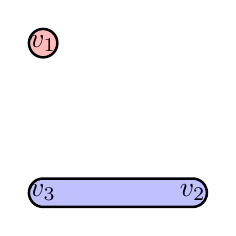
\begin{tikzpicture}[x=0.95cm,y=0.95cm]
  \fill[red!70, fill opacity=0.38] (0.000,2.000) circle[radius=0.19];
  \fill[blue!65, fill opacity=0.38] (0.000,0.190) arc[start angle=90.00, end angle=270.00, radius=0.19] -- (2.000,-0.190) arc[start angle=-90.00, end angle=90.00, radius=0.19] -- cycle;
  \draw[black, line width=0.9pt] (0.000,2.000) circle[radius=0.19];
  \draw[black, line width=0.9pt] (0.000,0.190) arc[start angle=90.00, end angle=270.00, radius=0.19] -- (2.000,-0.190) arc[start angle=-90.00, end angle=90.00, radius=0.19] -- cycle;
  \node[inner sep=0pt] at (0.000,2.000) {$v_{1}$};
  \node[inner sep=0pt] at (0.000,0.000) {$v_{3}$};
  \node[inner sep=0pt] at (2.000,0.000) {$v_{2}$};
\end{tikzpicture}
\caption{Hypergraph St\textsubscript{2}}\end{subfigure}\hfill
\begin{subfigure}{0.45\linewidth}\centering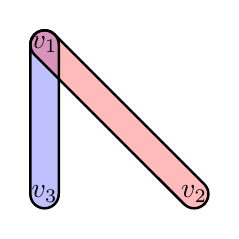
\begin{tikzpicture}[x=0.95cm,y=0.95cm]
  \fill[blue!65, fill opacity=0.38] (-0.190,0.000) arc[start angle=180.00, end angle=360.00, radius=0.19] -- (0.190,2.000) arc[start angle=0.00, end angle=180.00, radius=0.19] -- cycle;
  \fill[red!70, fill opacity=0.38] (0.134,2.134) arc[start angle=45.00, end angle=225.00, radius=0.19] -- (1.866,-0.134) arc[start angle=-135.00, end angle=45.00, radius=0.19] -- cycle;
  \draw[black, line width=0.9pt] (-0.190,0.000) arc[start angle=180.00, end angle=360.00, radius=0.19] -- (0.190,2.000) arc[start angle=0.00, end angle=180.00, radius=0.19] -- cycle;
  \draw[black, line width=0.9pt] (0.134,2.134) arc[start angle=45.00, end angle=225.00, radius=0.19] -- (1.866,-0.134) arc[start angle=-135.00, end angle=45.00, radius=0.19] -- cycle;
  \node[inner sep=0pt] at (0.000,2.000) {$v_{1}$};
  \node[inner sep=0pt] at (0.000,0.000) {$v_{3}$};
  \node[inner sep=0pt] at (2.000,0.000) {$v_{2}$};
\end{tikzpicture}
\caption{Transversal of St\textsubscript{2}}\end{subfigure}\\[8pt]
\begin{subfigure}{0.45\linewidth}\centering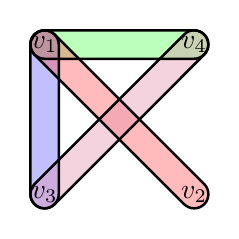
\begin{tikzpicture}[x=0.95cm,y=0.95cm]
  \fill[green!70, fill opacity=0.38] (0.000,2.190) arc[start angle=90.00, end angle=270.00, radius=0.19] -- (2.000,1.810) arc[start angle=-90.00, end angle=90.00, radius=0.19] -- cycle;
  \fill[blue!65, fill opacity=0.38] (-0.190,0.000) arc[start angle=180.00, end angle=360.00, radius=0.19] -- (0.190,2.000) arc[start angle=0.00, end angle=180.00, radius=0.19] -- cycle;
  \fill[red!70, fill opacity=0.38] (0.134,2.134) arc[start angle=45.00, end angle=225.00, radius=0.19] -- (1.866,-0.134) arc[start angle=-135.00, end angle=45.00, radius=0.19] -- cycle;
  \fill[purple!45, fill opacity=0.38] (-0.134,0.134) arc[start angle=135.00, end angle=315.00, radius=0.19] -- (2.134,1.866) arc[start angle=-45.00, end angle=135.00, radius=0.19] -- cycle;
  \draw[black, line width=0.9pt] (0.000,2.190) arc[start angle=90.00, end angle=270.00, radius=0.19] -- (2.000,1.810) arc[start angle=-90.00, end angle=90.00, radius=0.19] -- cycle;
  \draw[black, line width=0.9pt] (-0.190,0.000) arc[start angle=180.00, end angle=360.00, radius=0.19] -- (0.190,2.000) arc[start angle=0.00, end angle=180.00, radius=0.19] -- cycle;
  \draw[black, line width=0.9pt] (0.134,2.134) arc[start angle=45.00, end angle=225.00, radius=0.19] -- (1.866,-0.134) arc[start angle=-135.00, end angle=45.00, radius=0.19] -- cycle;
  \draw[black, line width=0.9pt] (-0.134,0.134) arc[start angle=135.00, end angle=315.00, radius=0.19] -- (2.134,1.866) arc[start angle=-45.00, end angle=135.00, radius=0.19] -- cycle;
  \node[inner sep=0pt] at (0.000,2.000) {$v_{1}$};
  \node[inner sep=0pt] at (2.000,2.000) {$v_{4}$};
  \node[inner sep=0pt] at (0.000,0.000) {$v_{3}$};
  \node[inner sep=0pt] at (2.000,0.000) {$v_{2}$};
\end{tikzpicture}
\caption{Hypergraph Pn\textsubscript{3}}\end{subfigure}\hfill
\begin{subfigure}{0.45\linewidth}\centering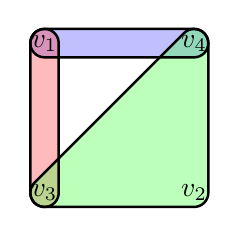
\begin{tikzpicture}[x=0.95cm,y=0.95cm]
  \fill[blue!65, fill opacity=0.38] (0.000,2.190) arc[start angle=90.00, end angle=270.00, radius=0.19] -- (2.000,1.810) arc[start angle=-90.00, end angle=90.00, radius=0.19] -- cycle;
  \fill[red!70, fill opacity=0.38] (-0.190,0.000) arc[start angle=180.00, end angle=360.00, radius=0.19] -- (0.190,2.000) arc[start angle=0.00, end angle=180.00, radius=0.19] -- cycle;
  \fill[green!70, fill opacity=0.38] (-0.134,0.134) arc[start angle=135.00, end angle=270.00, radius=0.19] -- (2.000,-0.190) arc[start angle=-90.00, end angle=0.00, radius=0.19] -- (2.190,2.000) arc[start angle=0.00, end angle=135.00, radius=0.19] -- cycle;
  \draw[black, line width=0.9pt] (0.000,2.190) arc[start angle=90.00, end angle=270.00, radius=0.19] -- (2.000,1.810) arc[start angle=-90.00, end angle=90.00, radius=0.19] -- cycle;
  \draw[black, line width=0.9pt] (-0.190,0.000) arc[start angle=180.00, end angle=360.00, radius=0.19] -- (0.190,2.000) arc[start angle=0.00, end angle=180.00, radius=0.19] -- cycle;
  \draw[black, line width=0.9pt] (-0.134,0.134) arc[start angle=135.00, end angle=270.00, radius=0.19] -- (2.000,-0.190) arc[start angle=-90.00, end angle=0.00, radius=0.19] -- (2.190,2.000) arc[start angle=0.00, end angle=135.00, radius=0.19] -- cycle;
  \node[inner sep=0pt] at (0.000,2.000) {$v_{1}$};
  \node[inner sep=0pt] at (2.000,2.000) {$v_{4}$};
  \node[inner sep=0pt] at (0.000,0.000) {$v_{3}$};
  \node[inner sep=0pt] at (2.000,0.000) {$v_{2}$};
\end{tikzpicture}
\caption{Transversal of Pn\textsubscript{3}}\end{subfigure}
\caption{Hypergraphs St\textsubscript{2} and Pn\textsubscript{3} and their transversals.}\label{fig:st2-pn3}
\end{figure}

In $\overline{Pn_3}$, the frequencies of $v_1,v_2,v_3$, and $v_4$ are $1$, $\frac{2}{3}$, $\frac{1}{2}$, and $\frac{1}{2}$, respectively \leanref{pn3bar_freq}. We see that all vertices of the hypergraph are above the frequency threshold of \FKA{} with $v_1$ being the most frequent. Choosing $v_1$ gives an instance of $St_2$ and $D_{1,0}$, whereas choosing $v_2$ gives instances of $D_{1,1}$ and interestingly, $D_{3,1}:\{\{v_1\},\{v_2\},\{v_3\}\},\{\{v_1,\mathbf{v_2},v_3\}\}$, and choosing $v_4$ or $v_3$ gives $St_2$ and $D_{2,1}$. While the hypergraph has the automorphism group $S_2$, decomposition can change it's automorphism group to $S_3$, giving us an instance of gaining symmetry in \FKA{} decomposition.

Lastly, in $Pn_3$, $v_1$ is the most frequent vertex, with frequency $\frac{3}{4}$, and $v_4$ and $v_3$ are frequent with frequency $\frac{2}{3}$ \leanref{pn3_freq}, while $v_2$ is considered infrequent and has frequency $\frac{1}{3}$ (see Figure \ref{fig:st2-pn3}). Here, removing $v_1$ gives optimal results, with an instance of $D_{1,2}$ and an instance of $D_{3,1}$. Choosing $v_2$, which is excluded by all but the most basic rule, produces the worst-case performance by instantiating $K_3$ and St\textsubscript{2}. Choosing $v_4$ or $v_3$ gives 5 nodes with St\textsubscript{2} and $D_{2,1}$.

\subsubsection*{Hypergraphs $G$ with $\Aut(G)\cong S_3$}

Up 3 vertices, hypergraphs such as $D_{1,1}$, $D_{3,1}:\{\{v_1\},\{v_2\},\{v_3\}\},\{\{v_1,\mathbf{v_2},v_3\}\}$, and $K_3:\{\{v_1,\mathbf{v_2}\},\{v_1,v_3\},\{v_2,v_3\}\}$ have automorphism groups isomorphic to $S_3$. Additionally, on 4 vertices, hypergraphs denoted
\begin{gather*}
St_3:\{\{v_1,v_2\},\{v_1,v_3\},\{v_1,v_4\}\},\{\{v_1\},\{v_2,v_3,v_4\}\},\\[4pt]
hw_3:\{\{v_1,v_4\},\{v_2,v_4\},\{v_3,v_4\},\{v_1,v_2,v_3\}\},\{\{v_1,v_4\},\{v_2,v_4\},\{v_3,v_4\},\{v_1,v_2,v_3\}\},\\[4pt]
K_3^{\cdot}:\{\{v_2\},\{v_1,v_3\},\{v_1,v_4\},\{v_3,v_4\}\},\{\{v_1,v_2,v_3\},\{v_1,v_2,v_4\},\{v_2,v_3,v_4\}\}.
\end{gather*}

\begin{figure}[tp]
\centering
\begin{subfigure}{0.45\linewidth}\centering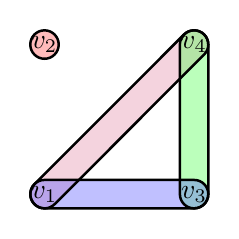
\begin{tikzpicture}[x=0.95cm,y=0.95cm]
  \fill[red!70, fill opacity=0.38] (0.000,2.000) circle[radius=0.19];
  \fill[purple!45, fill opacity=0.38] (-0.134,0.134) arc[start angle=135.00, end angle=315.00, radius=0.19] -- (2.134,1.866) arc[start angle=-45.00, end angle=135.00, radius=0.19] -- cycle;
  \fill[green!70, fill opacity=0.38] (1.810,0.000) arc[start angle=180.00, end angle=360.00, radius=0.19] -- (2.190,2.000) arc[start angle=0.00, end angle=180.00, radius=0.19] -- cycle;
  \fill[blue!65, fill opacity=0.38] (0.000,0.190) arc[start angle=90.00, end angle=270.00, radius=0.19] -- (2.000,-0.190) arc[start angle=-90.00, end angle=90.00, radius=0.19] -- cycle;
  \draw[black, line width=0.9pt] (0.000,2.000) circle[radius=0.19];
  \draw[black, line width=0.9pt] (-0.134,0.134) arc[start angle=135.00, end angle=315.00, radius=0.19] -- (2.134,1.866) arc[start angle=-45.00, end angle=135.00, radius=0.19] -- cycle;
  \draw[black, line width=0.9pt] (1.810,0.000) arc[start angle=180.00, end angle=360.00, radius=0.19] -- (2.190,2.000) arc[start angle=0.00, end angle=180.00, radius=0.19] -- cycle;
  \draw[black, line width=0.9pt] (0.000,0.190) arc[start angle=90.00, end angle=270.00, radius=0.19] -- (2.000,-0.190) arc[start angle=-90.00, end angle=90.00, radius=0.19] -- cycle;
  \node[inner sep=0pt] at (0.000,2.000) {$v_{2}$};
  \node[inner sep=0pt] at (2.000,2.000) {$v_{4}$};
  \node[inner sep=0pt] at (0.000,0.000) {$v_{1}$};
  \node[inner sep=0pt] at (2.000,0.000) {$v_{3}$};
\end{tikzpicture}
\caption{Hypergraph $K_3^{\cdot}$}\end{subfigure}\hfill
\begin{subfigure}{0.45\linewidth}\centering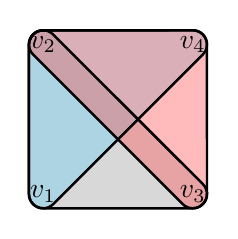
\begin{tikzpicture}[x=0.95cm,y=0.95cm]
  \fill[gray!80, fill opacity=0.38] (-0.190,0.000) arc[start angle=180.00, end angle=270.00, radius=0.19] -- (2.000,-0.190) arc[start angle=-90.00, end angle=45.00, radius=0.19] -- (0.134,2.134) arc[start angle=45.00, end angle=180.00, radius=0.19] -- cycle;
  \fill[cyan!60, fill opacity=0.38] (-0.190,0.000) arc[start angle=180.00, end angle=315.00, radius=0.19] -- (2.134,1.866) arc[start angle=-45.00, end angle=90.00, radius=0.19] -- (0.000,2.190) arc[start angle=90.00, end angle=180.00, radius=0.19] -- cycle;
  \fill[red!70, fill opacity=0.38] (0.000,2.190) arc[start angle=90.00, end angle=225.00, radius=0.19] -- (1.866,-0.134) arc[start angle=-135.00, end angle=0.00, radius=0.19] -- (2.190,2.000) arc[start angle=0.00, end angle=90.00, radius=0.19] -- cycle;
  \draw[black, line width=0.9pt] (-0.190,0.000) arc[start angle=180.00, end angle=270.00, radius=0.19] -- (2.000,-0.190) arc[start angle=-90.00, end angle=45.00, radius=0.19] -- (0.134,2.134) arc[start angle=45.00, end angle=180.00, radius=0.19] -- cycle;
  \draw[black, line width=0.9pt] (-0.190,0.000) arc[start angle=180.00, end angle=315.00, radius=0.19] -- (2.134,1.866) arc[start angle=-45.00, end angle=90.00, radius=0.19] -- (0.000,2.190) arc[start angle=90.00, end angle=180.00, radius=0.19] -- cycle;
  \draw[black, line width=0.9pt] (0.000,2.190) arc[start angle=90.00, end angle=225.00, radius=0.19] -- (1.866,-0.134) arc[start angle=-135.00, end angle=0.00, radius=0.19] -- (2.190,2.000) arc[start angle=0.00, end angle=90.00, radius=0.19] -- cycle;
  \node[inner sep=0pt] at (0.000,2.000) {$v_{2}$};
  \node[inner sep=0pt] at (2.000,2.000) {$v_{4}$};
  \node[inner sep=0pt] at (0.000,0.000) {$v_{1}$};
  \node[inner sep=0pt] at (2.000,0.000) {$v_{3}$};
\end{tikzpicture}
\caption{Transversal of $K_3^{\cdot}$}\end{subfigure}\\[8pt]
\begin{subfigure}{0.45\linewidth}\centering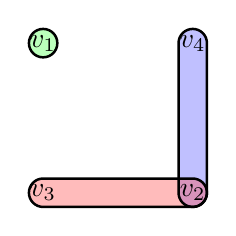
\begin{tikzpicture}[x=0.95cm,y=0.95cm]
  \fill[green!70, fill opacity=0.38] (0.000,2.000) circle[radius=0.19];
  \fill[blue!65, fill opacity=0.38] (1.810,0.000) arc[start angle=180.00, end angle=360.00, radius=0.19] -- (2.190,2.000) arc[start angle=0.00, end angle=180.00, radius=0.19] -- cycle;
  \fill[red!70, fill opacity=0.38] (0.000,0.190) arc[start angle=90.00, end angle=270.00, radius=0.19] -- (2.000,-0.190) arc[start angle=-90.00, end angle=90.00, radius=0.19] -- cycle;
  \draw[black, line width=0.9pt] (0.000,2.000) circle[radius=0.19];
  \draw[black, line width=0.9pt] (1.810,0.000) arc[start angle=180.00, end angle=360.00, radius=0.19] -- (2.190,2.000) arc[start angle=0.00, end angle=180.00, radius=0.19] -- cycle;
  \draw[black, line width=0.9pt] (0.000,0.190) arc[start angle=90.00, end angle=270.00, radius=0.19] -- (2.000,-0.190) arc[start angle=-90.00, end angle=90.00, radius=0.19] -- cycle;
  \node[inner sep=0pt] at (0.000,2.000) {$v_{1}$};
  \node[inner sep=0pt] at (2.000,2.000) {$v_{4}$};
  \node[inner sep=0pt] at (0.000,0.000) {$v_{3}$};
  \node[inner sep=0pt] at (2.000,0.000) {$v_{2}$};
\end{tikzpicture}
\caption{Hypergraph $\overline{\text{Pn}_3}$}\end{subfigure}\hfill
\begin{subfigure}{0.45\linewidth}\centering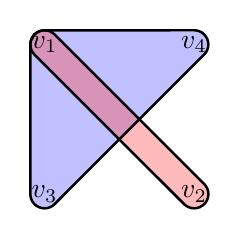
\begin{tikzpicture}[x=0.95cm,y=0.95cm]
  \fill[blue!65, fill opacity=0.38] (-0.190,0.000) arc[start angle=180.00, end angle=315.00, radius=0.19] -- (2.134,1.866) arc[start angle=-45.00, end angle=90.00, radius=0.19] -- (0.000,2.190) arc[start angle=90.00, end angle=180.00, radius=0.19] -- cycle;
  \fill[red!70, fill opacity=0.38] (0.134,2.134) arc[start angle=45.00, end angle=225.00, radius=0.19] -- (1.866,-0.134) arc[start angle=-135.00, end angle=45.00, radius=0.19] -- cycle;
  \draw[black, line width=0.9pt] (-0.190,0.000) arc[start angle=180.00, end angle=315.00, radius=0.19] -- (2.134,1.866) arc[start angle=-45.00, end angle=90.00, radius=0.19] -- (0.000,2.190) arc[start angle=90.00, end angle=180.00, radius=0.19] -- cycle;
  \draw[black, line width=0.9pt] (0.134,2.134) arc[start angle=45.00, end angle=225.00, radius=0.19] -- (1.866,-0.134) arc[start angle=-135.00, end angle=45.00, radius=0.19] -- cycle;
  \node[inner sep=0pt] at (0.000,2.000) {$v_{1}$};
  \node[inner sep=0pt] at (2.000,2.000) {$v_{4}$};
  \node[inner sep=0pt] at (0.000,0.000) {$v_{3}$};
  \node[inner sep=0pt] at (2.000,0.000) {$v_{2}$};
\end{tikzpicture}
\caption{Transversal of $\overline{\text{Pn}_3}$}\end{subfigure}
\caption{Hypergraph $K_3^{\cdot}$ and its transversal. Hypergraph $\overline{\text{Pn}_3}$ and its transversal.}\label{fig:k3dot-pn3bar}
\end{figure}

also have $S_3$ as their automorphism group (\leanref{table_aut}; transversals \leanref{st3_tr}, \leanref{hw3_tr}, \leanref{k3dot_tr}). The 2024 edition printed $K_3^{\cdot}$ with the edge $\{v_2,v_4\}$, which is not Sperner, and with transversal $\{\{v_1,v_2,v_3,v_4\}\}$ \leanref{k3dot_printed_not_sperner}.

In $St_3$, vertices $v_2$, $v_3$, and $v_4$ are frequent with frequency $\frac{1}{2}$, and $v_1$ is most frequent as it occurs in all edges (see Figure \ref{fig:d31-st3}). Removing $v_1$ results in a trivial instance of $D_{0,1}$ and $D_{3,1}$, while removing other vertices yields subhypergraphs isomorphic to $St_2$ or $D_{1,1}$. The first case results in a recursion tree with 3 nodes, whereas the latter ends up with 5 nodes.

Similarly, we see that in $hw_3$ (see Figure \ref{fig:p4-hw3}), $v_1$, $v_2$, and $v_3$ are frequent with frequency $\frac{1}{2}$ (\emph{frequent} in the context of multiple vertices having the same frequency and there existing a separate most frequent vertex) and $v_4$ is most frequent with frequency $\frac{3}{4}$ . Recursing on $v_4$ results in an instance of $D_{1,3}$, and an instance of $D_{3,1}$, thus the recursion tree of our modified implementation has 3 nodes. Choosing any other vertex leads to two instances of $St_2$, which has 3 nodes. So, the maximum size of the recursion tree is 7 nodes.

The hypergraph $K_3^{\cdot}$ is defined as a cycle $C_3$ together with a singleton vertex (see Figure \ref{fig:k3dot-pn3bar}). The vertex $v_2$ is most frequent with frequency 1, and the other vertices are frequent with a frequency of $\frac{2}{3}$. Removing $v_2$ gives $D_{0,1}$ and $K_3$ for a recursion tree with 5 nodes. Choosing any of the other vertices gives instances of $D_{1,3}$ and $St_2$, which again, results in a tree with 5 nodes.

Lastly, $K_3$ is invariant under any permutation and in general $\Aut(K_n)\cong S_n$ (see Figure \ref{fig:k3-k4minus}). Selecting $v_1$ as the splitting vertex, we get two cases of $D_{1,2}$, which are trivial due to our modifications, and once again we have a tree of size 3. Another interesting observation is that both $K_3$ and $hw_3$ are also self-transversal hypergraphs. In fact, the next well-known self-transversal hypergraph is on 7 vertices, namely the fano plane hypergraph, which is identified as a difficult case for \FKA.

\begin{figure}[tp]
\centering
\begin{subfigure}{0.45\linewidth}\centering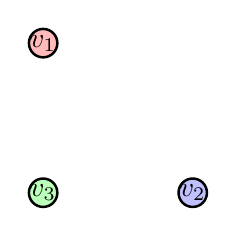
\begin{tikzpicture}[x=0.95cm,y=0.95cm]
  \fill[red!70, fill opacity=0.38] (0.000,2.000) circle[radius=0.19];
  \fill[green!70, fill opacity=0.38] (0.000,0.000) circle[radius=0.19];
  \fill[blue!65, fill opacity=0.38] (2.000,0.000) circle[radius=0.19];
  \draw[black, line width=0.9pt] (0.000,2.000) circle[radius=0.19];
  \draw[black, line width=0.9pt] (0.000,0.000) circle[radius=0.19];
  \draw[black, line width=0.9pt] (2.000,0.000) circle[radius=0.19];
  \node[inner sep=0pt] at (0.000,2.000) {$v_{1}$};
  \node[inner sep=0pt] at (0.000,0.000) {$v_{3}$};
  \node[inner sep=0pt] at (2.000,0.000) {$v_{2}$};
\end{tikzpicture}
\caption{Hypergraph $D_{3,1}$}\end{subfigure}\hfill
\begin{subfigure}{0.45\linewidth}\centering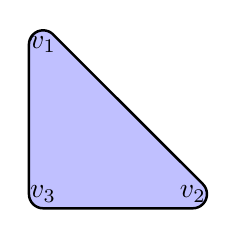
\begin{tikzpicture}[x=0.95cm,y=0.95cm]
  \fill[blue!65, fill opacity=0.38] (-0.190,0.000) arc[start angle=180.00, end angle=270.00, radius=0.19] -- (2.000,-0.190) arc[start angle=-90.00, end angle=45.00, radius=0.19] -- (0.134,2.134) arc[start angle=45.00, end angle=180.00, radius=0.19] -- cycle;
  \draw[black, line width=0.9pt] (-0.190,0.000) arc[start angle=180.00, end angle=270.00, radius=0.19] -- (2.000,-0.190) arc[start angle=-90.00, end angle=45.00, radius=0.19] -- (0.134,2.134) arc[start angle=45.00, end angle=180.00, radius=0.19] -- cycle;
  \node[inner sep=0pt] at (0.000,2.000) {$v_{1}$};
  \node[inner sep=0pt] at (0.000,0.000) {$v_{3}$};
  \node[inner sep=0pt] at (2.000,0.000) {$v_{2}$};
\end{tikzpicture}
\caption{Transversal of $D_{3,1}$}\end{subfigure}\\[8pt]
\begin{subfigure}{0.45\linewidth}\centering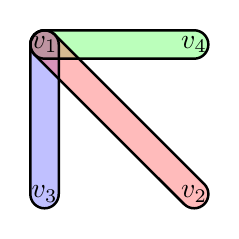
\begin{tikzpicture}[x=0.95cm,y=0.95cm]
  \fill[green!70, fill opacity=0.38] (0.000,2.190) arc[start angle=90.00, end angle=270.00, radius=0.19] -- (2.000,1.810) arc[start angle=-90.00, end angle=90.00, radius=0.19] -- cycle;
  \fill[blue!65, fill opacity=0.38] (-0.190,0.000) arc[start angle=180.00, end angle=360.00, radius=0.19] -- (0.190,2.000) arc[start angle=0.00, end angle=180.00, radius=0.19] -- cycle;
  \fill[red!70, fill opacity=0.38] (0.134,2.134) arc[start angle=45.00, end angle=225.00, radius=0.19] -- (1.866,-0.134) arc[start angle=-135.00, end angle=45.00, radius=0.19] -- cycle;
  \draw[black, line width=0.9pt] (0.000,2.190) arc[start angle=90.00, end angle=270.00, radius=0.19] -- (2.000,1.810) arc[start angle=-90.00, end angle=90.00, radius=0.19] -- cycle;
  \draw[black, line width=0.9pt] (-0.190,0.000) arc[start angle=180.00, end angle=360.00, radius=0.19] -- (0.190,2.000) arc[start angle=0.00, end angle=180.00, radius=0.19] -- cycle;
  \draw[black, line width=0.9pt] (0.134,2.134) arc[start angle=45.00, end angle=225.00, radius=0.19] -- (1.866,-0.134) arc[start angle=-135.00, end angle=45.00, radius=0.19] -- cycle;
  \node[inner sep=0pt] at (0.000,2.000) {$v_{1}$};
  \node[inner sep=0pt] at (2.000,2.000) {$v_{4}$};
  \node[inner sep=0pt] at (0.000,0.000) {$v_{3}$};
  \node[inner sep=0pt] at (2.000,0.000) {$v_{2}$};
\end{tikzpicture}
\caption{Hypergraph St\textsubscript{3}}\end{subfigure}\hfill
\begin{subfigure}{0.45\linewidth}\centering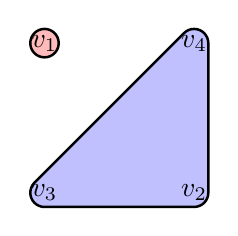
\begin{tikzpicture}[x=0.95cm,y=0.95cm]
  \fill[red!70, fill opacity=0.38] (0.000,2.000) circle[radius=0.19];
  \fill[blue!65, fill opacity=0.38] (-0.134,0.134) arc[start angle=135.00, end angle=270.00, radius=0.19] -- (2.000,-0.190) arc[start angle=-90.00, end angle=0.00, radius=0.19] -- (2.190,2.000) arc[start angle=0.00, end angle=135.00, radius=0.19] -- cycle;
  \draw[black, line width=0.9pt] (0.000,2.000) circle[radius=0.19];
  \draw[black, line width=0.9pt] (-0.134,0.134) arc[start angle=135.00, end angle=270.00, radius=0.19] -- (2.000,-0.190) arc[start angle=-90.00, end angle=0.00, radius=0.19] -- (2.190,2.000) arc[start angle=0.00, end angle=135.00, radius=0.19] -- cycle;
  \node[inner sep=0pt] at (0.000,2.000) {$v_{1}$};
  \node[inner sep=0pt] at (2.000,2.000) {$v_{4}$};
  \node[inner sep=0pt] at (0.000,0.000) {$v_{3}$};
  \node[inner sep=0pt] at (2.000,0.000) {$v_{2}$};
\end{tikzpicture}
\caption{Transversal of St\textsubscript{3}}\end{subfigure}
\caption{Hypergraph $D_{3,1}$ and its transversal. Hypergraph St\textsubscript{3} and its transversal.}\label{fig:d31-st3}
\end{figure}

\subsubsection*{Hypergraphs $G$ with $\Aut(G)\cong S_2\times S_2$}

Hypergraphs on 4 vertices with automorphism group isomorphic to $S_2\times S_2$ are denoted as $D_{2,1}$,
\[
K_4^-:\{\{v_3,v_4\},\{v_1,v_4\},\{v_1,v_3\},\{v_2,v_4\},\{v_2,v_3\}\},\{\{v_1,v_2,v_3\},\{v_1,v_2,v_4\},\{v_3,v_4\}\},
\]
\[
K_2^{\cdot\cdot}:\{\{v_1\},\{v_2\},\{v_3,v_4\}\},\{\{v_1,v_2,v_3\},\{v_1,v_2,v_4\}\}.
\]
The symmetry of hypergraphs $K_2^{\cdot\cdot}$ and $K_4^-$ is generated by permutations like $\langle(v_1,v_2),(v_3,v_4)\rangle$, i.e., we can either permute $(v_1,v_2)$ or $(v_3,v_4)$ or both (\leanref{k4minus_tr}, \leanref{k2dd_tr}). The 2024 edition printed the transversal of $K_4^-$ as $\{\{v_1,v_2,v_3,v_4\},\{v_1,v_2,v_4\},\{v_1,v_3,v_4\}\}$ and $K_2^{\cdot\cdot}$ as the self-paired $\{\{v_1,v_2\},\{v_3,v_4\}\}$; neither is a transversal pair (\leanref{k4minus_printed_not_tr}, \leanref{k2dd_printed_not_tr}).

$K_4^-$ is a complete graph on 4 vertices missing one edge, where all vertices have maximum frequency $\frac{2}{3}$ (see Figure \ref{fig:k3-k4minus}). Recursing on any vertex leads to hypergraphs such as $K_3$ and $D_{2,1}$, resulting in a recursion tree with 5 nodes.

$K_2^{\cdot\cdot}$ is the complete graph $K_2$ with two singleton vertices, with its transversal hypergraph having 2 edges each containing 3 vertices (see Figure \ref{fig:k2dd-c4}). $v_1$ and $v_2$ are most frequent with frequency 1, and $v_3$ and $v_4$ are frequent with frequency $\frac{1}{2}$. Choosing $v_3$ or $v_4$ gives an instance of $D_{3,1}$ and $D_{2,1}$, which results in 3 nodes in the recursion tree, while choosing $v_1$ or $v_2$ gives rise to $St_2$ and $D_{1,0}$, for a total of 5 nodes. Interestingly, in this case, choosing the vertex with the highest frequency is not optimal in terms of tree size \leanref{k2dd_mfv_not_optimal}.

\subsubsection*{Hypergraphs $G$ with $\Aut(G)\cong D_4$}

The cycle graph $C_4:\{\{v_1,v_2\},\{v_2,v_3\},\{v_3,v_4\},\{v_1,v_4\}\},\{\{v_1,v_3\},\{v_2,v_4\}\}$ \leanref{c4_tr} is invariant under both rotation and reflection, leading to the automorphism group $D_4$ (see Figure \ref{fig:k2dd-c4}). All vertices in $C_4$ are frequent, with no distinct most frequent vertex. Like $K_n$, each vertex is isomorphic, implying that removing any vertex gives isomorphic hypergraphs. Choosing any vertex produces an instance of $St_2$ and an instance of $D_{2,1}$, totaling five nodes in the tree.

\begin{figure}[tp]
\centering
\begin{subfigure}{0.45\linewidth}\centering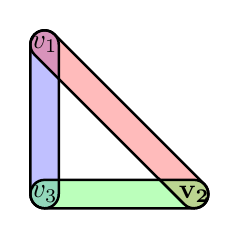
\begin{tikzpicture}[x=0.95cm,y=0.95cm]
  \fill[blue!65, fill opacity=0.38] (-0.190,0.000) arc[start angle=180.00, end angle=360.00, radius=0.19] -- (0.190,2.000) arc[start angle=0.00, end angle=180.00, radius=0.19] -- cycle;
  \fill[red!70, fill opacity=0.38] (0.134,2.134) arc[start angle=45.00, end angle=225.00, radius=0.19] -- (1.866,-0.134) arc[start angle=-135.00, end angle=45.00, radius=0.19] -- cycle;
  \fill[green!70, fill opacity=0.38] (0.000,0.190) arc[start angle=90.00, end angle=270.00, radius=0.19] -- (2.000,-0.190) arc[start angle=-90.00, end angle=90.00, radius=0.19] -- cycle;
  \draw[black, line width=0.9pt] (-0.190,0.000) arc[start angle=180.00, end angle=360.00, radius=0.19] -- (0.190,2.000) arc[start angle=0.00, end angle=180.00, radius=0.19] -- cycle;
  \draw[black, line width=0.9pt] (0.134,2.134) arc[start angle=45.00, end angle=225.00, radius=0.19] -- (1.866,-0.134) arc[start angle=-135.00, end angle=45.00, radius=0.19] -- cycle;
  \draw[black, line width=0.9pt] (0.000,0.190) arc[start angle=90.00, end angle=270.00, radius=0.19] -- (2.000,-0.190) arc[start angle=-90.00, end angle=90.00, radius=0.19] -- cycle;
  \node[inner sep=0pt] at (0.000,2.000) {$v_{1}$};
  \node[inner sep=0pt] at (0.000,0.000) {$v_{3}$};
  \node[inner sep=0pt] at (2.000,0.000) {$\mathbf{v_{2}}$};
\end{tikzpicture}
\caption{Hypergraph $K_3$}\end{subfigure}\hfill
\begin{subfigure}{0.45\linewidth}\centering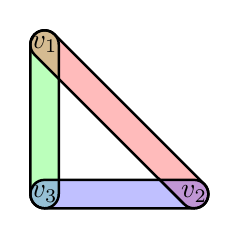
\begin{tikzpicture}[x=0.95cm,y=0.95cm]
  \fill[green!70, fill opacity=0.38] (-0.190,0.000) arc[start angle=180.00, end angle=360.00, radius=0.19] -- (0.190,2.000) arc[start angle=0.00, end angle=180.00, radius=0.19] -- cycle;
  \fill[red!70, fill opacity=0.38] (0.134,2.134) arc[start angle=45.00, end angle=225.00, radius=0.19] -- (1.866,-0.134) arc[start angle=-135.00, end angle=45.00, radius=0.19] -- cycle;
  \fill[blue!65, fill opacity=0.38] (0.000,0.190) arc[start angle=90.00, end angle=270.00, radius=0.19] -- (2.000,-0.190) arc[start angle=-90.00, end angle=90.00, radius=0.19] -- cycle;
  \draw[black, line width=0.9pt] (-0.190,0.000) arc[start angle=180.00, end angle=360.00, radius=0.19] -- (0.190,2.000) arc[start angle=0.00, end angle=180.00, radius=0.19] -- cycle;
  \draw[black, line width=0.9pt] (0.134,2.134) arc[start angle=45.00, end angle=225.00, radius=0.19] -- (1.866,-0.134) arc[start angle=-135.00, end angle=45.00, radius=0.19] -- cycle;
  \draw[black, line width=0.9pt] (0.000,0.190) arc[start angle=90.00, end angle=270.00, radius=0.19] -- (2.000,-0.190) arc[start angle=-90.00, end angle=90.00, radius=0.19] -- cycle;
  \node[inner sep=0pt] at (0.000,2.000) {$v_{1}$};
  \node[inner sep=0pt] at (0.000,0.000) {$v_{3}$};
  \node[inner sep=0pt] at (2.000,0.000) {$v_{2}$};
\end{tikzpicture}
\caption{Transversal of $K_3$}\end{subfigure}\\[8pt]
\begin{subfigure}{0.45\linewidth}\centering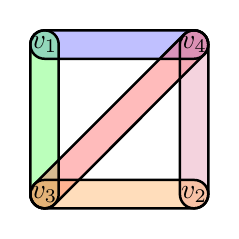
\begin{tikzpicture}[x=0.95cm,y=0.95cm]
  \fill[blue!65, fill opacity=0.38] (0.000,2.190) arc[start angle=90.00, end angle=270.00, radius=0.19] -- (2.000,1.810) arc[start angle=-90.00, end angle=90.00, radius=0.19] -- cycle;
  \fill[green!70, fill opacity=0.38] (-0.190,0.000) arc[start angle=180.00, end angle=360.00, radius=0.19] -- (0.190,2.000) arc[start angle=0.00, end angle=180.00, radius=0.19] -- cycle;
  \fill[red!70, fill opacity=0.38] (-0.134,0.134) arc[start angle=135.00, end angle=315.00, radius=0.19] -- (2.134,1.866) arc[start angle=-45.00, end angle=135.00, radius=0.19] -- cycle;
  \fill[purple!45, fill opacity=0.38] (1.810,0.000) arc[start angle=180.00, end angle=360.00, radius=0.19] -- (2.190,2.000) arc[start angle=0.00, end angle=180.00, radius=0.19] -- cycle;
  \fill[orange!70, fill opacity=0.38] (0.000,0.190) arc[start angle=90.00, end angle=270.00, radius=0.19] -- (2.000,-0.190) arc[start angle=-90.00, end angle=90.00, radius=0.19] -- cycle;
  \draw[black, line width=0.9pt] (0.000,2.190) arc[start angle=90.00, end angle=270.00, radius=0.19] -- (2.000,1.810) arc[start angle=-90.00, end angle=90.00, radius=0.19] -- cycle;
  \draw[black, line width=0.9pt] (-0.190,0.000) arc[start angle=180.00, end angle=360.00, radius=0.19] -- (0.190,2.000) arc[start angle=0.00, end angle=180.00, radius=0.19] -- cycle;
  \draw[black, line width=0.9pt] (-0.134,0.134) arc[start angle=135.00, end angle=315.00, radius=0.19] -- (2.134,1.866) arc[start angle=-45.00, end angle=135.00, radius=0.19] -- cycle;
  \draw[black, line width=0.9pt] (1.810,0.000) arc[start angle=180.00, end angle=360.00, radius=0.19] -- (2.190,2.000) arc[start angle=0.00, end angle=180.00, radius=0.19] -- cycle;
  \draw[black, line width=0.9pt] (0.000,0.190) arc[start angle=90.00, end angle=270.00, radius=0.19] -- (2.000,-0.190) arc[start angle=-90.00, end angle=90.00, radius=0.19] -- cycle;
  \node[inner sep=0pt] at (0.000,2.000) {$v_{1}$};
  \node[inner sep=0pt] at (2.000,2.000) {$v_{4}$};
  \node[inner sep=0pt] at (0.000,0.000) {$v_{3}$};
  \node[inner sep=0pt] at (2.000,0.000) {$v_{2}$};
\end{tikzpicture}
\caption{Hypergraph $K_4^-$}\end{subfigure}\hfill
\begin{subfigure}{0.45\linewidth}\centering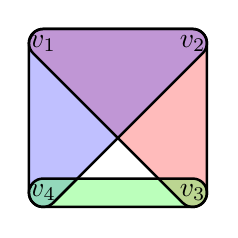
\begin{tikzpicture}[x=0.95cm,y=0.95cm]
  \fill[red!70, fill opacity=0.38] (0.000,2.190) arc[start angle=90.00, end angle=225.00, radius=0.19] -- (1.866,-0.134) arc[start angle=-135.00, end angle=0.00, radius=0.19] -- (2.190,2.000) arc[start angle=0.00, end angle=90.00, radius=0.19] -- cycle;
  \fill[blue!65, fill opacity=0.38] (-0.190,0.000) arc[start angle=180.00, end angle=315.00, radius=0.19] -- (2.134,1.866) arc[start angle=-45.00, end angle=90.00, radius=0.19] -- (0.000,2.190) arc[start angle=90.00, end angle=180.00, radius=0.19] -- cycle;
  \fill[green!70, fill opacity=0.38] (0.000,0.190) arc[start angle=90.00, end angle=270.00, radius=0.19] -- (2.000,-0.190) arc[start angle=-90.00, end angle=90.00, radius=0.19] -- cycle;
  \draw[black, line width=0.9pt] (0.000,2.190) arc[start angle=90.00, end angle=225.00, radius=0.19] -- (1.866,-0.134) arc[start angle=-135.00, end angle=0.00, radius=0.19] -- (2.190,2.000) arc[start angle=0.00, end angle=90.00, radius=0.19] -- cycle;
  \draw[black, line width=0.9pt] (-0.190,0.000) arc[start angle=180.00, end angle=315.00, radius=0.19] -- (2.134,1.866) arc[start angle=-45.00, end angle=90.00, radius=0.19] -- (0.000,2.190) arc[start angle=90.00, end angle=180.00, radius=0.19] -- cycle;
  \draw[black, line width=0.9pt] (0.000,0.190) arc[start angle=90.00, end angle=270.00, radius=0.19] -- (2.000,-0.190) arc[start angle=-90.00, end angle=90.00, radius=0.19] -- cycle;
  \node[inner sep=0pt] at (0.000,2.000) {$v_{1}$};
  \node[inner sep=0pt] at (2.000,2.000) {$v_{2}$};
  \node[inner sep=0pt] at (2.000,0.000) {$v_{3}$};
  \node[inner sep=0pt] at (0.000,0.000) {$v_{4}$};
\end{tikzpicture}
\caption{Transversal of $K_4^-$}\end{subfigure}
\caption{Hypergraph $K_3$ and its transversal. Hypergraph $K_4^-$ and its transversal.}\label{fig:k3-k4minus}
\end{figure}

\subsubsection*{Hypergraphs $G$ with $\Aut(G)\cong S_4$}

The hypergraphs
\[
D_{4,1}:\{\{v_1\},\{v_2\},\{v_3\},\{v_4\}\},\{\{\mathbf{v_1},\mathbf{v_2},\mathbf{v_3},\mathbf{v_4}\}\},
\]
\[
K_4:\{\{v_1,v_2\},\{v_2,v_3\},\{v_2,v_4\},\{v_1,v_3\},\{v_3,v_4\},\{v_1,v_4\}\},\{\{v_1,v_2,v_3\},\{v_1,v_2,v_4\},\{v_1,v_3,v_4\},\{v_2,v_3,v_4\}\}.
\]
and $D_{1,0}$ are invariant under any permutation. Consequently, their automorphism group is isomorphic to $S_4$.

Specifically, $K_4$ has complete symmetry with respect to permutations, and all vertices have frequency $\frac{3}{4}$. Therefore, choosing any splitting vertex during recursion results in two instances of $K_3$ and $D_{3,1}$, yielding a recursion tree with five nodes.

Altogether, on 4 vertices there are 30 equivalence classes, i.e.\ distinct hypergraphs under permutation (see Table 3.1) \leanref{classes_four}: 4 self-transversal classes and 13 pairs of classes $\{G,\Tr(G)\}$ with $G\not\cong\Tr(G)$ \leanref{self_dual_classes_four}. There are in total 168 distinct hypergraphs on 4 vertices (see Table 3.2) \leanref{sperner_four_card}, which are all permutations of the abovementioned structures. By elementary group theory, the number of different permutations of these hypergraphs is $\frac{24}{|G|}$, where $G$ is the automorphism group of the given hypergraph. There are $\binom{4}{k}$ permutations for $D_{k,1}$, $\binom{4}{3}\cdot 4=12$ permutations for $St_2$, and 4 permutations for $St_3$ and $hw_3$. Similarly, there are $\binom{4}{3}$ permutations for $K_3$, 6 for $K_4^-$,

\begin{figure}[tp]
\centering
\begin{subfigure}{0.45\linewidth}\centering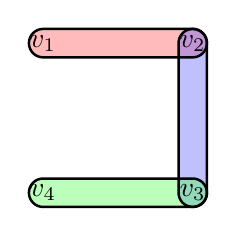
\begin{tikzpicture}[x=0.95cm,y=0.95cm]
  \fill[red!70, fill opacity=0.38] (0.000,2.190) arc[start angle=90.00, end angle=270.00, radius=0.19] -- (2.000,1.810) arc[start angle=-90.00, end angle=90.00, radius=0.19] -- cycle;
  \fill[blue!65, fill opacity=0.38] (1.810,0.000) arc[start angle=180.00, end angle=360.00, radius=0.19] -- (2.190,2.000) arc[start angle=0.00, end angle=180.00, radius=0.19] -- cycle;
  \fill[green!70, fill opacity=0.38] (0.000,0.190) arc[start angle=90.00, end angle=270.00, radius=0.19] -- (2.000,-0.190) arc[start angle=-90.00, end angle=90.00, radius=0.19] -- cycle;
  \draw[black, line width=0.9pt] (0.000,2.190) arc[start angle=90.00, end angle=270.00, radius=0.19] -- (2.000,1.810) arc[start angle=-90.00, end angle=90.00, radius=0.19] -- cycle;
  \draw[black, line width=0.9pt] (1.810,0.000) arc[start angle=180.00, end angle=360.00, radius=0.19] -- (2.190,2.000) arc[start angle=0.00, end angle=180.00, radius=0.19] -- cycle;
  \draw[black, line width=0.9pt] (0.000,0.190) arc[start angle=90.00, end angle=270.00, radius=0.19] -- (2.000,-0.190) arc[start angle=-90.00, end angle=90.00, radius=0.19] -- cycle;
  \node[inner sep=0pt] at (0.000,2.000) {$v_{1}$};
  \node[inner sep=0pt] at (2.000,2.000) {$v_{2}$};
  \node[inner sep=0pt] at (2.000,0.000) {$v_{3}$};
  \node[inner sep=0pt] at (0.000,0.000) {$v_{4}$};
\end{tikzpicture}
\caption{Hypergraph $P_4$}\end{subfigure}\hfill
\begin{subfigure}{0.45\linewidth}\centering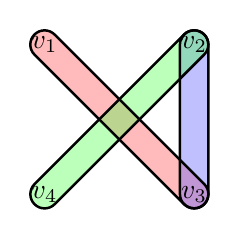
\begin{tikzpicture}[x=0.95cm,y=0.95cm]
  \fill[red!70, fill opacity=0.38] (0.134,2.134) arc[start angle=45.00, end angle=225.00, radius=0.19] -- (1.866,-0.134) arc[start angle=-135.00, end angle=45.00, radius=0.19] -- cycle;
  \fill[blue!65, fill opacity=0.38] (1.810,0.000) arc[start angle=180.00, end angle=360.00, radius=0.19] -- (2.190,2.000) arc[start angle=0.00, end angle=180.00, radius=0.19] -- cycle;
  \fill[green!70, fill opacity=0.38] (-0.134,0.134) arc[start angle=135.00, end angle=315.00, radius=0.19] -- (2.134,1.866) arc[start angle=-45.00, end angle=135.00, radius=0.19] -- cycle;
  \draw[black, line width=0.9pt] (0.134,2.134) arc[start angle=45.00, end angle=225.00, radius=0.19] -- (1.866,-0.134) arc[start angle=-135.00, end angle=45.00, radius=0.19] -- cycle;
  \draw[black, line width=0.9pt] (1.810,0.000) arc[start angle=180.00, end angle=360.00, radius=0.19] -- (2.190,2.000) arc[start angle=0.00, end angle=180.00, radius=0.19] -- cycle;
  \draw[black, line width=0.9pt] (-0.134,0.134) arc[start angle=135.00, end angle=315.00, radius=0.19] -- (2.134,1.866) arc[start angle=-45.00, end angle=135.00, radius=0.19] -- cycle;
  \node[inner sep=0pt] at (0.000,2.000) {$v_{1}$};
  \node[inner sep=0pt] at (2.000,2.000) {$v_{2}$};
  \node[inner sep=0pt] at (2.000,0.000) {$v_{3}$};
  \node[inner sep=0pt] at (0.000,0.000) {$v_{4}$};
\end{tikzpicture}
\caption{Transversal of $P_4$}\end{subfigure}\\[8pt]
\begin{subfigure}{0.45\linewidth}\centering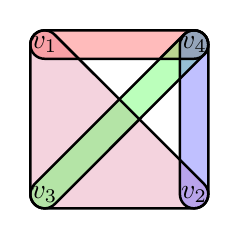
\begin{tikzpicture}[x=0.95cm,y=0.95cm]
  \fill[purple!45, fill opacity=0.38] (-0.190,0.000) arc[start angle=180.00, end angle=270.00, radius=0.19] -- (2.000,-0.190) arc[start angle=-90.00, end angle=45.00, radius=0.19] -- (0.134,2.134) arc[start angle=45.00, end angle=180.00, radius=0.19] -- cycle;
  \fill[red!70, fill opacity=0.38] (0.000,2.190) arc[start angle=90.00, end angle=270.00, radius=0.19] -- (2.000,1.810) arc[start angle=-90.00, end angle=90.00, radius=0.19] -- cycle;
  \fill[green!70, fill opacity=0.38] (-0.134,0.134) arc[start angle=135.00, end angle=315.00, radius=0.19] -- (2.134,1.866) arc[start angle=-45.00, end angle=135.00, radius=0.19] -- cycle;
  \fill[blue!65, fill opacity=0.38] (1.810,0.000) arc[start angle=180.00, end angle=360.00, radius=0.19] -- (2.190,2.000) arc[start angle=0.00, end angle=180.00, radius=0.19] -- cycle;
  \draw[black, line width=0.9pt] (-0.190,0.000) arc[start angle=180.00, end angle=270.00, radius=0.19] -- (2.000,-0.190) arc[start angle=-90.00, end angle=45.00, radius=0.19] -- (0.134,2.134) arc[start angle=45.00, end angle=180.00, radius=0.19] -- cycle;
  \draw[black, line width=0.9pt] (0.000,2.190) arc[start angle=90.00, end angle=270.00, radius=0.19] -- (2.000,1.810) arc[start angle=-90.00, end angle=90.00, radius=0.19] -- cycle;
  \draw[black, line width=0.9pt] (-0.134,0.134) arc[start angle=135.00, end angle=315.00, radius=0.19] -- (2.134,1.866) arc[start angle=-45.00, end angle=135.00, radius=0.19] -- cycle;
  \draw[black, line width=0.9pt] (1.810,0.000) arc[start angle=180.00, end angle=360.00, radius=0.19] -- (2.190,2.000) arc[start angle=0.00, end angle=180.00, radius=0.19] -- cycle;
  \node[inner sep=0pt] at (0.000,2.000) {$v_{1}$};
  \node[inner sep=0pt] at (2.000,2.000) {$v_{4}$};
  \node[inner sep=0pt] at (0.000,0.000) {$v_{3}$};
  \node[inner sep=0pt] at (2.000,0.000) {$v_{2}$};
\end{tikzpicture}
\caption{Hypergraph hw\textsubscript{3}}\end{subfigure}\hfill
\begin{subfigure}{0.45\linewidth}\centering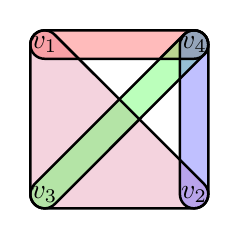
\begin{tikzpicture}[x=0.95cm,y=0.95cm]
  \fill[purple!45, fill opacity=0.38] (-0.190,0.000) arc[start angle=180.00, end angle=270.00, radius=0.19] -- (2.000,-0.190) arc[start angle=-90.00, end angle=45.00, radius=0.19] -- (0.134,2.134) arc[start angle=45.00, end angle=180.00, radius=0.19] -- cycle;
  \fill[red!70, fill opacity=0.38] (0.000,2.190) arc[start angle=90.00, end angle=270.00, radius=0.19] -- (2.000,1.810) arc[start angle=-90.00, end angle=90.00, radius=0.19] -- cycle;
  \fill[green!70, fill opacity=0.38] (-0.134,0.134) arc[start angle=135.00, end angle=315.00, radius=0.19] -- (2.134,1.866) arc[start angle=-45.00, end angle=135.00, radius=0.19] -- cycle;
  \fill[blue!65, fill opacity=0.38] (1.810,0.000) arc[start angle=180.00, end angle=360.00, radius=0.19] -- (2.190,2.000) arc[start angle=0.00, end angle=180.00, radius=0.19] -- cycle;
  \draw[black, line width=0.9pt] (-0.190,0.000) arc[start angle=180.00, end angle=270.00, radius=0.19] -- (2.000,-0.190) arc[start angle=-90.00, end angle=45.00, radius=0.19] -- (0.134,2.134) arc[start angle=45.00, end angle=180.00, radius=0.19] -- cycle;
  \draw[black, line width=0.9pt] (0.000,2.190) arc[start angle=90.00, end angle=270.00, radius=0.19] -- (2.000,1.810) arc[start angle=-90.00, end angle=90.00, radius=0.19] -- cycle;
  \draw[black, line width=0.9pt] (-0.134,0.134) arc[start angle=135.00, end angle=315.00, radius=0.19] -- (2.134,1.866) arc[start angle=-45.00, end angle=135.00, radius=0.19] -- cycle;
  \draw[black, line width=0.9pt] (1.810,0.000) arc[start angle=180.00, end angle=360.00, radius=0.19] -- (2.190,2.000) arc[start angle=0.00, end angle=180.00, radius=0.19] -- cycle;
  \node[inner sep=0pt] at (0.000,2.000) {$v_{1}$};
  \node[inner sep=0pt] at (2.000,2.000) {$v_{4}$};
  \node[inner sep=0pt] at (0.000,0.000) {$v_{3}$};
  \node[inner sep=0pt] at (2.000,0.000) {$v_{2}$};
\end{tikzpicture}
\caption{Transversal of hw\textsubscript{3}}\end{subfigure}
\caption{Hypergraph $P_4$ and its transversal. Hypergraph hw\textsubscript{3} and its transversal.}\label{fig:p4-hw3}
\end{figure}

\noindent and 1 permutation for $K_4$. The cycle $C_4$ has 3 permutations and $K_2^{\cdot\cdot}$ also has 6, while $K_3^{\cdot}$ has 4 permutations. $P_4$ has 12 permutations. Finally, $Pn_3$ and $\overline{Pn_3}$ are complementary graphs and both have 12 permutations. Adding these numbers up and taking note of self-transversal cases indeed gives us the 168 distinct hypergraphs.

The hypergraphs according to these symmetry groups are grouped in the following table:

\begin{table}[h]
\centering
\begin{tabular}{|c|c|}
\hline
$D_{4,1},K_4,D_{1,0}$ & $S_4$\\\hline
$C_4$ & $D_4$\\\hline
$D_{1,1},D_{3,1},\text{star}_3,hw_3,K_3,K_3^{\cdot}$ & $S_3$\\\hline
$D_{2,1},K_4^-,K_2^{\cdot\cdot}$ & $S_2\times S_2$\\\hline
$\text{star}_2,\text{pan}_3,\text{pan}_3',\text{path}_4$ & $S_2$\\\hline
\end{tabular}
\caption{Hypergraphs grouped by their automorphism groups (\leanref{table_aut}, \leanref{table_orbits}).}
\end{table}

\begin{figure}[tp]
\centering
\begin{subfigure}{0.45\linewidth}\centering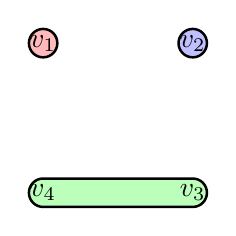
\begin{tikzpicture}[x=0.95cm,y=0.95cm]
  \fill[red!70, fill opacity=0.38] (0.000,2.000) circle[radius=0.19];
  \fill[blue!65, fill opacity=0.38] (2.000,2.000) circle[radius=0.19];
  \fill[green!70, fill opacity=0.38] (0.000,0.190) arc[start angle=90.00, end angle=270.00, radius=0.19] -- (2.000,-0.190) arc[start angle=-90.00, end angle=90.00, radius=0.19] -- cycle;
  \draw[black, line width=0.9pt] (0.000,2.000) circle[radius=0.19];
  \draw[black, line width=0.9pt] (2.000,2.000) circle[radius=0.19];
  \draw[black, line width=0.9pt] (0.000,0.190) arc[start angle=90.00, end angle=270.00, radius=0.19] -- (2.000,-0.190) arc[start angle=-90.00, end angle=90.00, radius=0.19] -- cycle;
  \node[inner sep=0pt] at (0.000,2.000) {$v_{1}$};
  \node[inner sep=0pt] at (2.000,2.000) {$v_{2}$};
  \node[inner sep=0pt] at (2.000,0.000) {$v_{3}$};
  \node[inner sep=0pt] at (0.000,0.000) {$v_{4}$};
\end{tikzpicture}
\caption{Hypergraph $K_2^{\cdot\cdot}$}\end{subfigure}\hfill
\begin{subfigure}{0.45\linewidth}\centering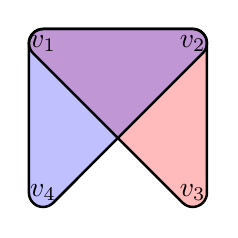
\begin{tikzpicture}[x=0.95cm,y=0.95cm]
  \fill[red!70, fill opacity=0.38] (0.000,2.190) arc[start angle=90.00, end angle=225.00, radius=0.19] -- (1.866,-0.134) arc[start angle=-135.00, end angle=0.00, radius=0.19] -- (2.190,2.000) arc[start angle=0.00, end angle=90.00, radius=0.19] -- cycle;
  \fill[blue!65, fill opacity=0.38] (-0.190,0.000) arc[start angle=180.00, end angle=315.00, radius=0.19] -- (2.134,1.866) arc[start angle=-45.00, end angle=90.00, radius=0.19] -- (0.000,2.190) arc[start angle=90.00, end angle=180.00, radius=0.19] -- cycle;
  \draw[black, line width=0.9pt] (0.000,2.190) arc[start angle=90.00, end angle=225.00, radius=0.19] -- (1.866,-0.134) arc[start angle=-135.00, end angle=0.00, radius=0.19] -- (2.190,2.000) arc[start angle=0.00, end angle=90.00, radius=0.19] -- cycle;
  \draw[black, line width=0.9pt] (-0.190,0.000) arc[start angle=180.00, end angle=315.00, radius=0.19] -- (2.134,1.866) arc[start angle=-45.00, end angle=90.00, radius=0.19] -- (0.000,2.190) arc[start angle=90.00, end angle=180.00, radius=0.19] -- cycle;
  \node[inner sep=0pt] at (0.000,2.000) {$v_{1}$};
  \node[inner sep=0pt] at (2.000,2.000) {$v_{2}$};
  \node[inner sep=0pt] at (2.000,0.000) {$v_{3}$};
  \node[inner sep=0pt] at (0.000,0.000) {$v_{4}$};
\end{tikzpicture}
\caption{Transversal of $K_2^{\cdot\cdot}$}\end{subfigure}\\[8pt]
\begin{subfigure}{0.45\linewidth}\centering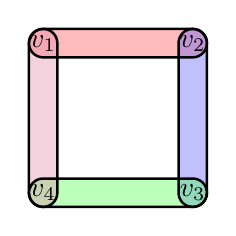
\begin{tikzpicture}[x=0.95cm,y=0.95cm]
  \fill[red!70, fill opacity=0.38] (0.000,2.190) arc[start angle=90.00, end angle=270.00, radius=0.19] -- (2.000,1.810) arc[start angle=-90.00, end angle=90.00, radius=0.19] -- cycle;
  \fill[blue!65, fill opacity=0.38] (1.810,0.000) arc[start angle=180.00, end angle=360.00, radius=0.19] -- (2.190,2.000) arc[start angle=0.00, end angle=180.00, radius=0.19] -- cycle;
  \fill[green!70, fill opacity=0.38] (0.000,0.190) arc[start angle=90.00, end angle=270.00, radius=0.19] -- (2.000,-0.190) arc[start angle=-90.00, end angle=90.00, radius=0.19] -- cycle;
  \fill[purple!45, fill opacity=0.38] (-0.190,0.000) arc[start angle=180.00, end angle=360.00, radius=0.19] -- (0.190,2.000) arc[start angle=0.00, end angle=180.00, radius=0.19] -- cycle;
  \draw[black, line width=0.9pt] (0.000,2.190) arc[start angle=90.00, end angle=270.00, radius=0.19] -- (2.000,1.810) arc[start angle=-90.00, end angle=90.00, radius=0.19] -- cycle;
  \draw[black, line width=0.9pt] (1.810,0.000) arc[start angle=180.00, end angle=360.00, radius=0.19] -- (2.190,2.000) arc[start angle=0.00, end angle=180.00, radius=0.19] -- cycle;
  \draw[black, line width=0.9pt] (0.000,0.190) arc[start angle=90.00, end angle=270.00, radius=0.19] -- (2.000,-0.190) arc[start angle=-90.00, end angle=90.00, radius=0.19] -- cycle;
  \draw[black, line width=0.9pt] (-0.190,0.000) arc[start angle=180.00, end angle=360.00, radius=0.19] -- (0.190,2.000) arc[start angle=0.00, end angle=180.00, radius=0.19] -- cycle;
  \node[inner sep=0pt] at (0.000,2.000) {$v_{1}$};
  \node[inner sep=0pt] at (2.000,2.000) {$v_{2}$};
  \node[inner sep=0pt] at (2.000,0.000) {$v_{3}$};
  \node[inner sep=0pt] at (0.000,0.000) {$v_{4}$};
\end{tikzpicture}
\caption{Hypergraph $C_4$}\end{subfigure}\hfill
\begin{subfigure}{0.45\linewidth}\centering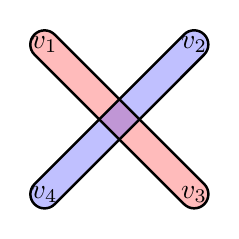
\begin{tikzpicture}[x=0.95cm,y=0.95cm]
  \fill[red!70, fill opacity=0.38] (0.134,2.134) arc[start angle=45.00, end angle=225.00, radius=0.19] -- (1.866,-0.134) arc[start angle=-135.00, end angle=45.00, radius=0.19] -- cycle;
  \fill[blue!65, fill opacity=0.38] (-0.134,0.134) arc[start angle=135.00, end angle=315.00, radius=0.19] -- (2.134,1.866) arc[start angle=-45.00, end angle=135.00, radius=0.19] -- cycle;
  \draw[black, line width=0.9pt] (0.134,2.134) arc[start angle=45.00, end angle=225.00, radius=0.19] -- (1.866,-0.134) arc[start angle=-135.00, end angle=45.00, radius=0.19] -- cycle;
  \draw[black, line width=0.9pt] (-0.134,0.134) arc[start angle=135.00, end angle=315.00, radius=0.19] -- (2.134,1.866) arc[start angle=-45.00, end angle=135.00, radius=0.19] -- cycle;
  \node[inner sep=0pt] at (0.000,2.000) {$v_{1}$};
  \node[inner sep=0pt] at (2.000,2.000) {$v_{2}$};
  \node[inner sep=0pt] at (2.000,0.000) {$v_{3}$};
  \node[inner sep=0pt] at (0.000,0.000) {$v_{4}$};
\end{tikzpicture}
\caption{Transversal of $C_4$}\end{subfigure}
\caption{Hypergraph $K_2^{\cdot\cdot}$ and its transversal. Hypergraph $C_4$ and its transversal.}\label{fig:k2dd-c4}
\end{figure}

\begin{figure}[tp]
\centering
\begin{subfigure}{0.45\linewidth}\centering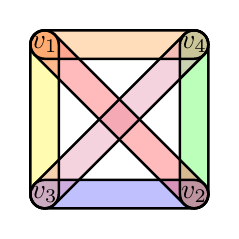
\begin{tikzpicture}[x=0.95cm,y=0.95cm]
  \fill[orange!70, fill opacity=0.38] (0.000,2.190) arc[start angle=90.00, end angle=270.00, radius=0.19] -- (2.000,1.810) arc[start angle=-90.00, end angle=90.00, radius=0.19] -- cycle;
  \fill[yellow!80, fill opacity=0.38] (-0.190,0.000) arc[start angle=180.00, end angle=360.00, radius=0.19] -- (0.190,2.000) arc[start angle=0.00, end angle=180.00, radius=0.19] -- cycle;
  \fill[green!70, fill opacity=0.38] (1.810,0.000) arc[start angle=180.00, end angle=360.00, radius=0.19] -- (2.190,2.000) arc[start angle=0.00, end angle=180.00, radius=0.19] -- cycle;
  \fill[blue!65, fill opacity=0.38] (0.000,0.190) arc[start angle=90.00, end angle=270.00, radius=0.19] -- (2.000,-0.190) arc[start angle=-90.00, end angle=90.00, radius=0.19] -- cycle;
  \fill[red!70, fill opacity=0.38] (0.134,2.134) arc[start angle=45.00, end angle=225.00, radius=0.19] -- (1.866,-0.134) arc[start angle=-135.00, end angle=45.00, radius=0.19] -- cycle;
  \fill[purple!45, fill opacity=0.38] (-0.134,0.134) arc[start angle=135.00, end angle=315.00, radius=0.19] -- (2.134,1.866) arc[start angle=-45.00, end angle=135.00, radius=0.19] -- cycle;
  \draw[black, line width=0.9pt] (0.000,2.190) arc[start angle=90.00, end angle=270.00, radius=0.19] -- (2.000,1.810) arc[start angle=-90.00, end angle=90.00, radius=0.19] -- cycle;
  \draw[black, line width=0.9pt] (-0.190,0.000) arc[start angle=180.00, end angle=360.00, radius=0.19] -- (0.190,2.000) arc[start angle=0.00, end angle=180.00, radius=0.19] -- cycle;
  \draw[black, line width=0.9pt] (1.810,0.000) arc[start angle=180.00, end angle=360.00, radius=0.19] -- (2.190,2.000) arc[start angle=0.00, end angle=180.00, radius=0.19] -- cycle;
  \draw[black, line width=0.9pt] (0.000,0.190) arc[start angle=90.00, end angle=270.00, radius=0.19] -- (2.000,-0.190) arc[start angle=-90.00, end angle=90.00, radius=0.19] -- cycle;
  \draw[black, line width=0.9pt] (0.134,2.134) arc[start angle=45.00, end angle=225.00, radius=0.19] -- (1.866,-0.134) arc[start angle=-135.00, end angle=45.00, radius=0.19] -- cycle;
  \draw[black, line width=0.9pt] (-0.134,0.134) arc[start angle=135.00, end angle=315.00, radius=0.19] -- (2.134,1.866) arc[start angle=-45.00, end angle=135.00, radius=0.19] -- cycle;
  \node[inner sep=0pt] at (0.000,2.000) {$v_{1}$};
  \node[inner sep=0pt] at (2.000,2.000) {$v_{4}$};
  \node[inner sep=0pt] at (0.000,0.000) {$v_{3}$};
  \node[inner sep=0pt] at (2.000,0.000) {$v_{2}$};
\end{tikzpicture}
\caption{Hypergraph $K_4$}\end{subfigure}\hfill
\begin{subfigure}{0.45\linewidth}\centering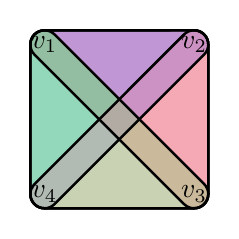
\begin{tikzpicture}[x=0.95cm,y=0.95cm]
  \fill[red!70, fill opacity=0.38] (0.000,2.190) arc[start angle=90.00, end angle=225.00, radius=0.19] -- (1.866,-0.134) arc[start angle=-135.00, end angle=0.00, radius=0.19] -- (2.190,2.000) arc[start angle=0.00, end angle=90.00, radius=0.19] -- cycle;
  \fill[blue!65, fill opacity=0.38] (-0.190,0.000) arc[start angle=180.00, end angle=315.00, radius=0.19] -- (2.134,1.866) arc[start angle=-45.00, end angle=90.00, radius=0.19] -- (0.000,2.190) arc[start angle=90.00, end angle=180.00, radius=0.19] -- cycle;
  \fill[green!70, fill opacity=0.38] (-0.190,0.000) arc[start angle=180.00, end angle=270.00, radius=0.19] -- (2.000,-0.190) arc[start angle=-90.00, end angle=45.00, radius=0.19] -- (0.134,2.134) arc[start angle=45.00, end angle=180.00, radius=0.19] -- cycle;
  \fill[purple!45, fill opacity=0.38] (-0.134,0.134) arc[start angle=135.00, end angle=270.00, radius=0.19] -- (2.000,-0.190) arc[start angle=-90.00, end angle=0.00, radius=0.19] -- (2.190,2.000) arc[start angle=0.00, end angle=135.00, radius=0.19] -- cycle;
  \draw[black, line width=0.9pt] (0.000,2.190) arc[start angle=90.00, end angle=225.00, radius=0.19] -- (1.866,-0.134) arc[start angle=-135.00, end angle=0.00, radius=0.19] -- (2.190,2.000) arc[start angle=0.00, end angle=90.00, radius=0.19] -- cycle;
  \draw[black, line width=0.9pt] (-0.190,0.000) arc[start angle=180.00, end angle=315.00, radius=0.19] -- (2.134,1.866) arc[start angle=-45.00, end angle=90.00, radius=0.19] -- (0.000,2.190) arc[start angle=90.00, end angle=180.00, radius=0.19] -- cycle;
  \draw[black, line width=0.9pt] (-0.190,0.000) arc[start angle=180.00, end angle=270.00, radius=0.19] -- (2.000,-0.190) arc[start angle=-90.00, end angle=45.00, radius=0.19] -- (0.134,2.134) arc[start angle=45.00, end angle=180.00, radius=0.19] -- cycle;
  \draw[black, line width=0.9pt] (-0.134,0.134) arc[start angle=135.00, end angle=270.00, radius=0.19] -- (2.000,-0.190) arc[start angle=-90.00, end angle=0.00, radius=0.19] -- (2.190,2.000) arc[start angle=0.00, end angle=135.00, radius=0.19] -- cycle;
  \node[inner sep=0pt] at (0.000,2.000) {$v_{1}$};
  \node[inner sep=0pt] at (2.000,2.000) {$v_{2}$};
  \node[inner sep=0pt] at (2.000,0.000) {$v_{3}$};
  \node[inner sep=0pt] at (0.000,0.000) {$v_{4}$};
\end{tikzpicture}
\caption{Transversal of $K_4$}\end{subfigure}
\caption{Hypergraph $K_4$ and its transversal.}\label{fig:k4}
\end{figure}

\section{Impact of \FKA{} on Symmetry}

We can understand how the symmetry within the hypergraph gets impacted when \FKA{} decomposes and recurses on input hypergraphs $G$, $H$ to test whether they are mutually transversals or not from the following discussion.

\begin{lemma}[\leanref{aut_tr_of_sperner}]\label{lem:aut-tr}
Suppose $\Aut(H)=\mathcal{G}$ for a Sperner hypergraph $H$ and its transversal hypergraph is denoted $\Tr(H)$. Then $\Aut(\Tr(H))=\mathcal{G}$. For an arbitrary hypergraph, $\Aut(\Tr(H))=\Aut(min(H))$ \leanref{aut_tr_eq_aut_minimal}.
\end{lemma}

The Sperner hypergraph is needed: for $H=\{\{v_1\},\{v_1,v_2\}\}$ on three vertices, $(v_2\,v_3)$ is an automorphism of $\Tr(H)=\{\{v_1\}\}$ but not of $H$ \leanref{lemma_3_3_1_needs_sperner}.

\begin{proof}
Suppose not. Let $\mathcal{G}'=\Aut(\Tr(H))$, and assume $\mathcal{G}\neq\mathcal{G}'$. Then there exists an automorphism $\phi$ such that either $\phi\in\mathcal{G}$ but $\phi\notin\mathcal{G}'$, or $\phi\in\mathcal{G}'$ but $\phi\notin\mathcal{G}$.

Suppose $\phi\in\mathcal{G}$ but $\phi\notin\mathcal{G}'$. Since $\phi\in\mathcal{G}$, it preserves the edge structure of $H$, mapping each hyperedge $e\in E(H)$ to another hyperedge $\phi(e)\in E(H)$. Now, for any minimal transversal $t\in\Tr(H)$, $\phi(t)$ intersects every hyperedge $\phi(e)$ of $H$, and as $\phi$ is a bijection, $\phi(t)$ remains minimal. Thus, $\phi(t)\in\Tr(H)$, implying $\phi\in\mathcal{G}'$, which contradicts the assumption.

If $\phi\in\mathcal{G}'$, the same argument applied to $\Tr(H)$ gives $\phi\in\Aut(\Tr(\Tr(H)))$, and $\Tr(\Tr(H))=H$ because $H$ is Sperner (Corollary 2.1.3). Hence, $\mathcal{G}=\mathcal{G}'$.
\end{proof}

\begin{lemma}[\leanref{aut_child_moves_split_to_isolated}, \leanref{stab_mem_aut_del}, \leanref{stab_mem_aut_con}]\label{lem:break}
Let \FKA{} split a pair on the vertex $v_i$. In both subproblems, before and after Sperner reduction, $v_i$ lies in no hyperedge, so an automorphism of a subproblem can move $v_i$ only to a vertex that also lies in no hyperedge of that subproblem. Every automorphism of the parent that fixes $v_i$ is an automorphism of both subproblems.
\end{lemma}

The 2024 edition stated this lemma informally, as the elimination of all automorphism generators containing $v_i$. The statement above is what holds; its proof replaces the one below, which is kept as printed for the record.

\begin{proof}
Let $H=(V,E)$ and $\Tr(H)=(V,E')$ be Sperner hypergraphs with a common vertex set $V$, where $E=\{e_1,e_2,\dots\}$ and $E'=\{t_1,t_2,\dots\}$ represent the edge sets of $H$ and $\Tr(H)$, respectively. Suppose $|H|\cdot|\Tr(H)|\geq 2$, and let $v_i$ be the most frequent vertex, occurring in either $H$ or $\Tr(H)$ with frequency at least $\frac{1}{\log(|H|+|\Tr(H)|)}$. Assume there exists a nontrivial automorphism generator $\sigma$ acting on both $H$ and $\Tr(H)$.

By definition, $\sigma$ is an automorphism generator, creating other automorphisms through composition, and it induces a permutation of vertices that forms nontrivial orbits within $V$. These orbits represent structural dependencies among vertices, as vertices within the same orbit are indistinguishable under the automorphisms generated by $\sigma$. The \FKA{} decomposition selects $v_i$, the most frequent vertex, and deletes it, effectively breaking the generator $\sigma$.

If $v_i$ is part of multiple automorphism generators, its removal disrupts the composition of these generators. Specifically, for a generator such as $(ab)(cd)$, deleting $v_i=a$ removes $a$ from the orbit, effectively separating the generator into $(cd)$. This action breaks the combined structure of the generators, rendering automorphisms generated through their composition invalid. As a result, all symmetries dependent on $v_i$ collapse, ensuring that no nontrivial automorphisms involving $v_i$ remain in the decomposed hypergraphs.
\end{proof}

The 2024 edition followed with a lemma asserting that symmetries independent of $v_i$ survive the split. It is false:

\begin{example}[\leanref{lemma_3_3_3_false}]
Let $G=\{\{v_1,v_3\},\{v_2,v_4\}\}$. Then $(v_1\,v_2)(v_3\,v_4)\in\Aut(G)$, and \FKA{} splits on $v_1$. The transposition $(v_3\,v_4)$ belongs to a different cycle of this automorphism than $v_1$, yet it is an automorphism of neither subproblem, before or after Sperner reduction.
\end{example}

For the record, the printed lemma read:

\begin{lemma}[false; see the example above]\label{lem:independent}
Let $H$ and $\Tr(H)$ be transversal hypergraphs with vertex set $V$. Suppose $v_i$ and $v_j$ are distinct vertices of $H$, and let $\sigma$ be an automorphism generator of $H$. If $v_i$ and $v_j$ do not belong to the same transposition of vertices within $\sigma$, deleting $v_i$ does not affect symmetries involving $v_j$. Specifically, if $\sigma\cong\langle(v_i\,v_k)(v_j\,v_m)\rangle$, removing $v_i$ breaks transpositions involving $v_i$, such as $(v_iv_k)$ from all automorphisms in $\Aut(H)$, but leaves other transpositions like $(v_jv_m)$ intact, preserving symmetries associated with $v_j$.
\end{lemma}

\begin{proof}
Let $H=(V,E)$ and $\Tr(H)=(V,E')$ be Sperner hypergraphs that are transversal to each other. Consider distinct vertices $v_i$ and $v_j$ in $V$, and let $\sigma$ be an automorphism generator of $H$. The relationship between $v_i$ and $v_j$ within $\sigma$ can be described as the following:

If $v_i$ and $v_j$ are in the same transposition within $\sigma$, such as $\sigma\cong\langle(v_i\,v_j)\rangle$, removing $v_i$ directly breaks the transposition $(v_i\,v_j)$. This action invalidates all automorphisms involving both $v_i$ and $v_j$, as their symmetry depends entirely on the transposition $(v_i\,v_j)$. The decomposition, therefore, eliminates all symmetries related to $v_j$ in this case.

If $v_i$ and $v_j$ are in different transpositions within the same generator, such as $\sigma\cong\langle(v_i\,v_k)(v_j\,v_m)\rangle$, the transpositions $(v_i\,v_k)$ and $(v_j\,v_m)$ are independent. Removing $v_i$ invalidates all automorphisms generated by $(v_i\,v_k)$ but does not affect the ones generated by $(v_j\,v_m)$. In this case, the decomposition breaks automorphisms involving $v_i$ while leaving all symmetries associated with $v_j$ intact.

If $v_i$ and $v_j$ belong to different generators, such as $\sigma_1\cong\langle(v_i\,v_k)\rangle$ and $\sigma_2\cong\langle(v_j\,v_m)\rangle$, the automorphic structures of $v_i$ and $v_j$ are completely independent. Removing $v_i$ affects only $\sigma_1$ by breaking $(v_i\,v_k)$, while $\sigma_2$ and its transposition $(v_j\,v_m)$ remain unaffected. The decomposition, in this case, does not impact the symmetries involving $v_j$.

Thus, in \FKA{} decomposition, removing $v_i$ breaks symmetries involving $v_i$ while preserving those associated with $v_j$, provided $v_i$ and $v_j$ are not part of the same transposition.
\end{proof}

\begin{corollary}[\leanref{aut_le_aut_minimal}]\label{cor:aut-min}
Let $min(H)$ be the Sperner reduced hypergraph of $H$. Then $\Aut(H)\le\Aut(min(H))$.
\end{corollary}

The 2024 edition claimed $\Aut(H)\cong\Aut(min(H))$. For $H=\{\{v_1\},\{v_1,v_2\}\}$ on three vertices, $|\Aut(H)|=1$ and $|\Aut(min(H))|=2$ \leanref{cor_3_3_4_not_iso}. The first paragraph of the proof below is correct; the second is not, because a superset of an edge need not be an edge.

\begin{proof}
Consider the Sperner reduced hypergraph $min(H)=(V,E)$. Let's show that if $\sigma\in\Aut(H)$, then $\sigma\in\Aut(min(H))$. By definition, $\sigma\in\Aut(H)$ maps each hyperedge in $E(H)$ to another hyperedge in $E(H)$. For any $e_i\in E_{min}(H)$, $\sigma(e_i)$ must also belong to $E(H)$. Suppose $\sigma(e_i)\notin E_{min}(H)$; then there exists $e_j\in E(H)$ such that $e_j\subset\sigma(e_i)$. Applying $\sigma^{-1}$, this implies $\sigma^{-1}(e_j)\subset e_i$, contradicting the minimality of $e_i$ in $min(H)$. Thus, $\sigma(e_i)\in E_{min}(H)$, proving that $\sigma$ preserves minimal hyperedges, so $\sigma\in\Aut(min(H))$.

Now, suppose that $\sigma\in\Aut(min(H))$. Then, it ensures that $\sigma$ maps each minimal hyperedge $e_i\in E_{min}(H)$ to another minimal hyperedge in $E_{min}(H)$. For any $e_i\in E(H)$, if $e_i\in E_{min}(H)$, then $\sigma(e_i)\in E_{min}(H)\subset E(H)$. If $e_i\notin E_{min}(H)$, $e_i$ must be a superset of some $e_j\in E_{min}(H)$. Since $\sigma$ preserves $E_{min}(H)$, $\sigma(e_j)\in E_{min}(H)$, making $\sigma(e_i)$ a superset of $\sigma(e_j)$ and ensuring $\sigma(e_i)\in E(H)$. Therefore, $\sigma(E(H))=E(H)$, and $\sigma\in\Aut(H)$.

Thus, $\Aut(H)\cong\Aut(min(H))$.
\end{proof}

\section{Primal Graph of A Hypergraph and \FKA{} Recursion}

\begin{definition}
The \emph{primal graph} of a hypergraph $H=(V,E)$, denoted $G(H)$, is the graph with the same vertex set $V$, where two vertices $u,v\in V$ are adjacent if and only if they appear together in at least one hyperedge $e\in E$.
\end{definition}

Primal graphs are also known as co-occurrence graphs, [2]-sections of hypergraphs, and Gaifman graphs in the literature \cite{DPP18}.

\begin{definition}
A hypergraph $H=(V,E(H))$ is \emph{conformal} if every maximal clique in its primal graph $G(H)$ is a hyperedge of $H$.
\end{definition}

For a conformal hypergraph $H=(V,E)$ and its primal graph $G(H)$, the clique hypergraph of $G(H)$ (\ref{def:clique}) is exactly $H$. Primal graph of a hypergraph represents the symmetric and structural properties of the hypergraph rather faithfully for conformal hypergraphs, as $G$ is uniquely determined if and only if $H$ is conformal. \cite{GMR06}. Since for conformal hypergraphs, every maximal clique in $G$ corresponds to a hyperedge in $H$, analyzing the cliques of $G$ can reveal key properties about hypergraph. For general hypergraphs, the primal graph $G$ does not uniquely determine it because multiple hypergraphs can share the same primal graph. The hyperedges of a general hypergraph may involve overlapping edges where the primal graph cannot distinguish the separate edges from the cliques of $G$.

With conformality, looking at the primal graph and how they they interact through the \FKA{} recursion can give us an insight into whether the induced subgraph preserved or display any characteristics through the decomposition. Graph minor operations are a well-known method to generate induced subgraphs from a graph. Generalizing this for hypergraphs, we get:

A hypergraph $H'$ is a \emph{minor} of $H$, denoted $H'\preceq H$, if $H'$ is obtained by:
\begin{itemize}
\item Deleting a vertex.
\item Deleting proper subhyperedges $e_j\subset e_i$, $e_i\in E(H)$.
\item Shrinking a 2-edge (adjacent vertices in $G(H)$) into a single vertex.
\end{itemize}

For a pair of Sperner hypergraphs $(F,H)$, the \emph{contraction} (\ref{def:contraction}) of $v\in V(F)$ results in:
\begin{align*}
F'&=\left(V(F)\setminus\{v\},\{e_i=e_j\setminus\{v\}\mid e_j\in E(F)\}\right),\\
H'&=\left(V(F)\cap V(H)\setminus\{v\},\{e_i=e_j\setminus\{v\}\mid e_j\in E(H)\cap V(F)\}\right).
\end{align*}
If $V(F)=V(H)=V$, this simplifies to:
\begin{align*}
F'&=\left(V\setminus\{v\},\{e_i=e_j\setminus\{v\}\mid e_j\in E(F)\}\right),\\
H'&=\left(V\setminus\{v\},\{e_i=e_j\setminus\{v\}\mid e_j\in E(H)\}\right).
\end{align*}

The \emph{deletion} (\ref{def:deletion}) of $v$ results in:
\begin{align*}
F'&=\left(V\setminus\{v\},\{e_i\in E(F)\mid v\notin e_i\}\right),\\
H'&=\left(V\setminus\{v\},\{e_i=e_j\setminus\{v\}\mid e_j\in E(H)\}\right).
\end{align*}
\cite{BS15}.

A \textbf{minor map} $\mu:F\to F'$ satisfies the following:
\begin{itemize}
\item $\mu(v)\cap\mu(u)=\emptyset$ for all distinct $u,v\in V(F)$,
\item $\{v\in V(F)\mid\mu(v)\cap e_j\neq\emptyset\}\subseteq e_i$ or $\emptyset$, for some $e_i\in E(F)$, for all $e_j\in E(F')$.
\end{itemize}

$F'\preceq F$ if and only if there exists $\mu$ such that $F'$ is formed as:
\[
F'=\bigcup_{v\in V(F')}F[\mu(v)]\cup\bigcup_{e\in E(F)}\mu(e).
\]

For hypergraph pairs $(F,H)$ and $(F',H')$, $(F,H)\preceq(F',H')$ if and only if there exists a minor map $\mu:(F,H)\to(F',H')$.

Therefore, minor operations on a hypergraph $H$ extends to its primal graph, denoted $G(H)$. However, the converse does not hold, as primal graphs do not fully preserve hypergraph structure.

\begin{example}
Let $H=(V,E)$ be a Sperner hypergraph where $V=\{v_1,v_2,v_3,v_4\}$ and $E=\{e_1,e_2,e_3\}$ with:
\[
e_1=\{v_1,v_2,v_3\},\quad e_2=\{v_2,v_4\},\quad e_3=\{v_3,v_4\}.
\]
The primal graph $G(H)$ has vertex set $V$ and edges:
\[
\{v_1,v_2\},\{v_1,v_3\},\{v_2,v_3\},\{v_2,v_4\},\{v_3,v_4\}.
\]

Consider the automorphism $\alpha\in\Aut(G(H))$ defined as:
\[
\alpha(v_1)=v_4,\quad\alpha(v_2)=v_2,\quad\alpha(v_3)=v_3,\quad\alpha(v_4)=v_1.
\]

This permutation preserves adjacency in $G(H)$ but maps the hyperedges of $H$ as:
\[
\alpha(e_1)=\{v_4,v_2,v_3\},\quad\alpha(e_2)=\{v_2,v_1\},\quad\alpha(e_3)=\{v_3,v_1\}.
\]
The 2024 edition used $\alpha=(v_1\,v_3)$, which is not an automorphism of $G(H)$: it sends the edge $\{v_3,v_4\}$ to the non-edge $\{v_1,v_4\}$ \leanref{ex34_corrected}.
While $\alpha$ is valid in $G(H)$, it fails to preserve the hyperedge structure of $H$. Thus, $\alpha\in\Aut(G(H))$, but $\alpha\notin\Aut(H)$.
\end{example}

\cite{AGT12} established the connection between hypergraph minors and their primal graphs with the following lemma:

\begin{lemma}
For Sperner hypergraphs $H,H'$, $H'\preceq H\iff(G(H'),H')\preceq(G(H),H)$.
\end{lemma}

To illustrate this, let the hypergraphs $G^{\emptyset}$ and $G^1$ be defined as:
\[
G^{\emptyset}=(V,\emptyset),\quad G^1=(V,E(G^1)),\quad E(G^1)=\{\{v\}\mid v\in V\}.
\]
Here, $G^{\emptyset}$ corresponds to the empty hypergraph, and $G^1$ corresponds to the singleton hypergraph, where each edge contains a single vertex. For any two graphs $G(H)$ and $G(H')$, the following equivalence holds:
\[
G(H')\preceq G(H)\iff(G(H'),G(H')^{\emptyset})\preceq(G(H),G(H)^{\emptyset})\iff(G(H'),G(H')^1)\preceq(G(H),G(H)^1).
\]
This demonstrates that hypergraph minor operations extend to their primal graphs. Therefore, we note the following:

\begin{observation}[\leanref{primal_children_le}]
Let \FKA{} split the pair $(C,D)$ on $v$. The primal graph of each subproblem, after Sperner reduction, is a subgraph of $G(C)-v$ or of $G(D)-v$. It is therefore a minor of the parent's primal graph, obtained by deleting $v$ and edges only.
\end{observation}

The \FKA{} algorithm recursively decomposes input hypergraphs $F$ and $H$ into subproblems corresponding to the contraction and deletion subhypergraphs $F'$ and $H'$. These operations extend to the primal graphs $G(F)$ and $G(H)$, resulting in the minors $G(F')$ and $G(H')$.

The decomposition proceeds until reaching end states: the empty graph $G^{\emptyset}=(V,\emptyset)$ and the singleton hypergraph $G^1=(V,E(G^1))$, where $E(G^1)=\{\{v\}\mid v\in V\}$.

In the next chapters, we explore the primal graph structures of poorly performing hypergraph classes in \FKA, examining their symmetry and properties preserved during decomposition.

\section{Symmetry in \FKA{} Recursion}

\FKA{} recursion process involves a decomposition, creating two smaller subproblems. To understand the effect of this operation on the symmetric structure of the input hypergraphs, it suffices to analyze the symmetry of one of the input hypergraphs, say $G$. By transversality, the other hypergraph $H$ will inherit symmetry restrictions from $G$. Depending on whether the input hypergraphs $G$ and $H$ have a nontrivial automorphism group and the choice of the vertex $v_i$, hypergraphs in \FKA{} recursion can gain symmetry, lose symmetry, or no changes in symmetry.

The minor operation \textbf{L} applied to $G$ produces a subhypergraph $G_1$ by deleting a vertex $v_i$ and all hyperedges incident to it while \textbf{R} contains $G_0\vee G_1$. Looking at the symmetric changes in \textbf{L} on $G$ to get $G_1$ is sufficient considering a similar operation can be described for $H$ and $H_1$ which is the transversal of $G_0\vee G_1$ and has the same symmetry. This operation can affect the automorphism group of $G$ in three distinct ways:

First, the hypergraph can \emph{gain} symmetry. Suppose $G_1$ has a new automorphism $\sigma$ such that $\sigma\notin\Aut(G)$. For $\sigma$ to permute two vertices $u,v\in V(G_1)$, the deletion of $v_i$ must remove hyperedges that previously prevented this symmetry. Specifically, in the hyperedges of $G$ incident to $v_i$, there must exist a structural conflict where $\sigma(u)\neq v$, meaning $u$ and $v$ were distinguished in $G$ but become indistinguishable in $G_1$ after the removal of $v_i$. This situation leads to a larger automorphism group for $G_1$ compared to $G$.

Second, the hypergraph can \emph{lose} symmetry. Suppose $G$ has a nontrivial automorphism group, and $\sigma\in\Aut(G)$. If $v_i$ participates in transpositions or permutations that are part of a generator of $\Aut(G)$, then removing $v_i$ invalidates all symmetries involving $v_i$. For example, if $\sigma$ contains a transposition $(v_i\,u)$, deleting $v_i$ disrupts the symmetry, reducing the automorphism group of $G_1$ to a subgroup of $\Aut(G)$. This case is rigorously outlined in \ref{lem:break}.

Finally, the symmetry of the hypergraph may remain \emph{unchanged}. If the vertex $v_i$ being removed does not participate in any transpositions within the automorphism group of $G$, the automorphism group of $G_1$ will be identical to $\Aut(G)$. This is explained in \ref{lem:independent}.

Understanding the nature of induced symmetries during \FKA{} recursion is challenging due to their hierarchical and modular structure. As we can see, depending on the choice of vertex, a variety of symmetries or no symmetries might emerge.

\chapter{Hard Classes of Hypergraphs for \FKA}

Fredman and Khachiyan derived upper bounds on the number of recursive calls in \ref{lem:subproblems} by bounding the smallest edge size and vertex frequency in the input hypergraphs \ref{obs:tight} \cite{FK96}. These bounds showed that \TransHyp{} is not NP-hard. Otherwise, any problem in NP could be solved in quasi-polynomial time, which is considered highly unlikely. Takata presented a super-polynomial lower bound of $n^{\Omega(\log\log n)}$ for Berge's algorithm (which solves the \emph{generation}-version of the problem), using the \emph{alternating trees} as an example \cite{Tak08}.

The term \emph{Alternating Trees} in the context of hypergraph transversals was used in \cite{GK99} to describe a family of hypergraphs used to prove the upper bounds of \FKA. Identifying challenging hypergraph classes, including Alternating Trees, has remained a problem of interest. A different description of alternating trees was later presented in \cite{Tak08}, describing another family of hypergraphs. Hertel unified both descriptions to propose a generalized Alternating Trees family in \cite{Her04}, conjecturing that these hypergraphs are challenging for \FKA{} and presented a superpolynomial upper bound of $n^{\omega(\log^{1-\mathcal{O}(1)}n)}$ on the number of subproblems.

\section{Hypergraph Operations}

Let $G=(V,E(G))$ and $H=(V,E(H))$ be two hypergraphs, where $E(G)=\{e_1,e_2,\dots,e_m\}$ and $E(H)=\{f_1,f_2,\dots,f_{m'}\}$. Using $\vee$ and $\wedge$ as binary operators on the edge sets of the hypergraphs, we can construct two new hypergraphs as follows:
\begin{itemize}
\item $G\vee H$: This hypergraph has $V(G\vee H)=V(G)\cup V(H)$ and $E(G\vee H)=E(G)\cup E(H)=\{e_1,e_2,\dots,e_m,f_1,f_2,\dots,f_{m'}\}$.
\item $G\wedge H$: This hypergraph has $V(G\wedge H)=V(G)\cup V(H)$ and $E(G\wedge H)=\{e\wedge f:e\in E(G),f\in E(H)\}=\{e_i\wedge f_j:i=1,\dots,m,j=1,\dots,m'\}$.
\end{itemize}

The minimal transversals of $G\vee H$ and $G\wedge H$ relate to the minimal transversals of $G$ and $H$ as follows \cite{Ber87}:
\begin{itemize}
\item $\Tr(G\vee H)=min(\Tr(G)\wedge\Tr(H))$ \ref{def:sperner-reduction},
\item $\Tr(G\wedge H)=min(\Tr(G)\vee\Tr(H))$
\end{itemize}
If $G$ and $H$ do not share any vertices, every edge in $\Tr(G)$ is disjoint from every edge in $\Tr(H)$. Thus:
\begin{itemize}
\item $\Tr(G\vee H)=\Tr(G)\wedge\Tr(H)$, and $|\Tr(G\vee H)|=|\Tr(G)|\cdot|\Tr(H)|$,
\item $\Tr(G\wedge H)=\Tr(G)\vee\Tr(H)$, and $|\Tr(G\wedge H)|=|\Tr(G)|+|\Tr(H)|$.
\end{itemize}
\cite{Tak08}

Berge presented and proved this construction in \cite{Ber87}. \cite{KS03} also presented this construction for their solution to \FKA.

\section{Alternating Trees}\label{sec:alternating}

\subsection{$\GK$-family}

Gurvich and Khachiyan presented an example of such a class of hypergraphs in \cite{GK99} for whom, in \FKA, the bounds are tight up to a factor of 2. They denoted the family of hypergraphs $f_k$ and their transversal hypergraphs $g_k$ as \emph{alternating trees.} We will call them \emph{$\GK$-family.}

Let $f_k$ be denoted as the collection of hypergraphs on $2^{2k-1}$ vertices defined by the following recursion:
\begin{align*}
&f_1=v_1\vee v_2,\\
&f_2=((v_1\vee v_2)\wedge(v_3\vee v_4))\vee((v_5\vee v_6)\wedge(v_7\vee v_8)),\\
&\quad\vdots\\
&f_{k+1}=((f_k(v_1,\dots,v_{n(k)})\wedge f_k(v_{n(k)+1},\dots,v_{2n(k)}))\vee(f_k(v_{2n(k)+1},\dots,v_{3n(k)})\wedge f_k(v_{3n(k)+1},\dots,v_{4n(k)})).
\end{align*}

Here, let $f_2$ be expressed as $(A_1\wedge A_2)\vee(A_3\wedge A_4)$, where $A_i$ $(i=1,\dots,4)$ are vertex-disjoint copies of $f_1$. Then, $f_k$ can be recursively written as:
\[
f_1=v_1\vee v_2,\quad f_k=(A_1\wedge A_2)\vee(A_3\wedge A_4).
\]

The corresponding transversal hypergraph for $f_k$, denoted $g_k$ are defined by the following recurrence:
\begin{align*}
g_1&=v_1\wedge v_2,\\
g_2&=((v_1\wedge v_2)\vee(v_3\wedge v_4))\wedge((v_5\wedge v_6)\vee(v_7\wedge v_8)),\\
&\ \,\vdots\\
g_{k+1}&=(g_k(v_1,\dots,v_{n(k)})\vee g_k(v_{n(k)+1},\dots,v_{2n(k)}))\wedge\\
&\quad\ (g_k(v_{2n(k)+1},\dots,v_{3n(k)})\vee g_k(v_{3n(k)+1},\dots,v_{4n(k)})).
\end{align*}

Similarly, we denote $g_2=(A_1\vee A_2)\wedge(A_3\vee A_4)$, where $A_i,i=1,\dots,4$ are disjoint copies of $g_1$, and get the following recursive form of $g_k$:
\[
g_1=v_1\wedge v_2,\quad g_k\ \ =(A_1\vee A_2)\wedge(A_3\vee A_4).
\]

\begin{figure}[h]
\centering
\begin{subfigure}{0.42\linewidth}\centering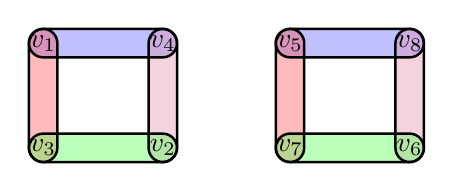
\begin{tikzpicture}[x=0.95cm,y=0.95cm]
  \fill[blue!65, fill opacity=0.38] (0.000,1.590) arc[start angle=90.00, end angle=270.00, radius=0.19] -- (1.600,1.210) arc[start angle=-90.00, end angle=90.00, radius=0.19] -- cycle;
  \fill[red!70, fill opacity=0.38] (-0.190,0.000) arc[start angle=180.00, end angle=360.00, radius=0.19] -- (0.190,1.400) arc[start angle=0.00, end angle=180.00, radius=0.19] -- cycle;
  \fill[purple!45, fill opacity=0.38] (1.410,0.000) arc[start angle=-180.00, end angle=-0.00, radius=0.19] -- (1.790,1.400) arc[start angle=-0.00, end angle=180.00, radius=0.19] -- cycle;
  \fill[green!70, fill opacity=0.38] (0.000,0.190) arc[start angle=90.00, end angle=270.00, radius=0.19] -- (1.600,-0.190) arc[start angle=-90.00, end angle=90.00, radius=0.19] -- cycle;
  \fill[blue!65, fill opacity=0.38] (3.300,1.590) arc[start angle=90.00, end angle=270.00, radius=0.19] -- (4.900,1.210) arc[start angle=-90.00, end angle=90.00, radius=0.19] -- cycle;
  \fill[red!70, fill opacity=0.38] (3.110,0.000) arc[start angle=-180.00, end angle=-0.00, radius=0.19] -- (3.490,1.400) arc[start angle=-0.00, end angle=180.00, radius=0.19] -- cycle;
  \fill[purple!45, fill opacity=0.38] (4.710,0.000) arc[start angle=-180.00, end angle=-0.00, radius=0.19] -- (5.090,1.400) arc[start angle=-0.00, end angle=180.00, radius=0.19] -- cycle;
  \fill[green!70, fill opacity=0.38] (3.300,0.190) arc[start angle=90.00, end angle=270.00, radius=0.19] -- (4.900,-0.190) arc[start angle=-90.00, end angle=90.00, radius=0.19] -- cycle;
  \draw[black, line width=0.9pt] (0.000,1.590) arc[start angle=90.00, end angle=270.00, radius=0.19] -- (1.600,1.210) arc[start angle=-90.00, end angle=90.00, radius=0.19] -- cycle;
  \draw[black, line width=0.9pt] (-0.190,0.000) arc[start angle=180.00, end angle=360.00, radius=0.19] -- (0.190,1.400) arc[start angle=0.00, end angle=180.00, radius=0.19] -- cycle;
  \draw[black, line width=0.9pt] (1.410,0.000) arc[start angle=-180.00, end angle=-0.00, radius=0.19] -- (1.790,1.400) arc[start angle=-0.00, end angle=180.00, radius=0.19] -- cycle;
  \draw[black, line width=0.9pt] (0.000,0.190) arc[start angle=90.00, end angle=270.00, radius=0.19] -- (1.600,-0.190) arc[start angle=-90.00, end angle=90.00, radius=0.19] -- cycle;
  \draw[black, line width=0.9pt] (3.300,1.590) arc[start angle=90.00, end angle=270.00, radius=0.19] -- (4.900,1.210) arc[start angle=-90.00, end angle=90.00, radius=0.19] -- cycle;
  \draw[black, line width=0.9pt] (3.110,0.000) arc[start angle=-180.00, end angle=-0.00, radius=0.19] -- (3.490,1.400) arc[start angle=-0.00, end angle=180.00, radius=0.19] -- cycle;
  \draw[black, line width=0.9pt] (4.710,0.000) arc[start angle=-180.00, end angle=-0.00, radius=0.19] -- (5.090,1.400) arc[start angle=-0.00, end angle=180.00, radius=0.19] -- cycle;
  \draw[black, line width=0.9pt] (3.300,0.190) arc[start angle=90.00, end angle=270.00, radius=0.19] -- (4.900,-0.190) arc[start angle=-90.00, end angle=90.00, radius=0.19] -- cycle;
  \node[inner sep=0pt] at (0.000,1.400) {$v_{1}$};
  \node[inner sep=0pt] at (1.600,1.400) {$v_{4}$};
  \node[inner sep=0pt] at (0.000,0.000) {$v_{3}$};
  \node[inner sep=0pt] at (1.600,0.000) {$v_{2}$};
  \node[inner sep=0pt] at (3.300,1.400) {$v_{5}$};
  \node[inner sep=0pt] at (4.900,1.400) {$v_{8}$};
  \node[inner sep=0pt] at (3.300,0.000) {$v_{7}$};
  \node[inner sep=0pt] at (4.900,0.000) {$v_{6}$};
\end{tikzpicture}
\caption{$f_2$}\end{subfigure}\hfill
\begin{subfigure}{0.5\linewidth}\centering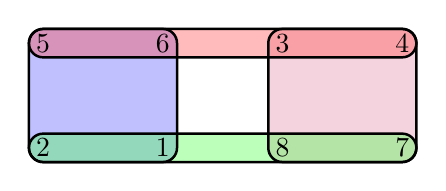
\begin{tikzpicture}[x=0.95cm,y=0.95cm]
  \fill[blue!65, fill opacity=0.38] (-0.190,0.000) arc[start angle=180.00, end angle=270.00, radius=0.19] -- (1.600,-0.190) arc[start angle=-90.00, end angle=-0.00, radius=0.19] -- (1.790,1.400) arc[start angle=-0.00, end angle=90.00, radius=0.19] -- (0.000,1.590) arc[start angle=90.00, end angle=180.00, radius=0.19] -- cycle;
  \fill[purple!45, fill opacity=0.38] (3.010,0.000) arc[start angle=-180.00, end angle=-90.00, radius=0.19] -- (4.800,-0.190) arc[start angle=-90.00, end angle=-0.00, radius=0.19] -- (4.990,1.400) arc[start angle=-0.00, end angle=90.00, radius=0.19] -- (3.200,1.590) arc[start angle=90.00, end angle=180.00, radius=0.19] -- cycle;
  \fill[red!70, fill opacity=0.38] (0.000,1.590) arc[start angle=90.00, end angle=270.00, radius=0.19] -- (4.800,1.210) arc[start angle=-90.00, end angle=90.00, radius=0.19] -- cycle;
  \fill[green!70, fill opacity=0.38] (0.000,0.190) arc[start angle=90.00, end angle=270.00, radius=0.19] -- (4.800,-0.190) arc[start angle=-90.00, end angle=90.00, radius=0.19] -- cycle;
  \draw[black, line width=0.9pt] (-0.190,0.000) arc[start angle=180.00, end angle=270.00, radius=0.19] -- (1.600,-0.190) arc[start angle=-90.00, end angle=-0.00, radius=0.19] -- (1.790,1.400) arc[start angle=-0.00, end angle=90.00, radius=0.19] -- (0.000,1.590) arc[start angle=90.00, end angle=180.00, radius=0.19] -- cycle;
  \draw[black, line width=0.9pt] (3.010,0.000) arc[start angle=-180.00, end angle=-90.00, radius=0.19] -- (4.800,-0.190) arc[start angle=-90.00, end angle=-0.00, radius=0.19] -- (4.990,1.400) arc[start angle=-0.00, end angle=90.00, radius=0.19] -- (3.200,1.590) arc[start angle=90.00, end angle=180.00, radius=0.19] -- cycle;
  \draw[black, line width=0.9pt] (0.000,1.590) arc[start angle=90.00, end angle=270.00, radius=0.19] -- (4.800,1.210) arc[start angle=-90.00, end angle=90.00, radius=0.19] -- cycle;
  \draw[black, line width=0.9pt] (0.000,0.190) arc[start angle=90.00, end angle=270.00, radius=0.19] -- (4.800,-0.190) arc[start angle=-90.00, end angle=90.00, radius=0.19] -- cycle;
  \node[inner sep=0pt] at (0.000,1.400) {$5$};
  \node[inner sep=0pt] at (1.600,1.400) {$6$};
  \node[inner sep=0pt] at (3.200,1.400) {$3$};
  \node[inner sep=0pt] at (4.800,1.400) {$4$};
  \node[inner sep=0pt] at (0.000,0.000) {$2$};
  \node[inner sep=0pt] at (1.600,0.000) {$1$};
  \node[inner sep=0pt] at (3.200,0.000) {$8$};
  \node[inner sep=0pt] at (4.800,0.000) {$7$};
\end{tikzpicture}
\caption{$g_2$}\end{subfigure}
\caption{Hypergraphs $f_2$ and $g_2$ in the $\GK$-family.}
\end{figure}

\subsection{$\TK$-family}

Takata denoted a class of recursively defined hypergraphs and their transversals as \emph{alternating trees} as well. We will address them as $\TK$-family. The set of hypergraphs $S_k\in\TK$ is defined recursively as follows:
\[
S_0=v_1,\quad S_1=(v_1\vee v_2)\wedge(v_3\vee v_4).
\]
For $k\geq 2$, $S_k$ is constructed as:
\[
S_k=(A\vee B)\wedge(C\vee D),
\]
where $A,B,C,D$ are vertex-disjoint copies of $S_{k-1}$.

The transversal hypergraph of $S_k$, denoted $r_k$, is defined recursively as follows:
\[
r_0=v_1,\quad r_1=(v_1\wedge v_2)\vee(v_3\wedge v_4).
\]
For $k\geq 2$, $r_k$ is constructed as:
\[
r_k=(A_1\wedge A_2)\vee(A_3\wedge A_4),
\]
where $A_i$, $i=1,\dots,4$ are vertex-disjoint copies of $r_{k-1}$.

\subsection{Combined Alternating Trees}

Hertel defined the combined alternating trees recursively as follows:
\[
\Gamma_0=\{v\},\quad\Gamma_i=\begin{cases}A\wedge B&\text{if }i\text{ odd},\\A\vee B&\text{if }i\text{ even.}\end{cases}
\]
where $A$ and $B$ are vertex-disjoint copies of $\Gamma_{i-1}$, and $\{v\}$ represents a hypergraph with a single edge containing one vertex. \cite{Her04}

The alternating tree $\Gamma_i$ corresponds to a hypergraph $H_i$ with $2^i$ vertices, forming a binary tree of height $i$, where each leaf represents a distinct vertex. They correspond to specific hypergraph families: $\GK$-family for odd $i$, and $\TK$-family for even $i$.

Denoting the set of edges of hypergraphs $H_i$ as $E_i$, we have:
\[
|E_0|=1,\quad|E_i|=\begin{cases}|E_{i-1}|^2&\text{if }i\text{ is odd,}\\2\times|E_{i-1}|&\text{if }i\text{ is even,}\end{cases}\qquad|E_i|=2^{2^{i/2}-1}\text{ for even }i.
\]

Similarly, denoting the set of transversals (edges in $\Tr(H_i)$) as $E_i'$, when $\Tr(H)$ is generated by $\Gamma_i$:
\[
|E_0'|=1,\quad|E_i'|=\begin{cases}2\times|E_{i-1}'|&\text{if }i\text{ is odd,}\\|E_{i-1}'|^2&\text{if }i\text{ is even,}\end{cases}\qquad|E_i'|=2^{2^{i/2+1}-2}\text{ for even }i.
\]
These are \leanref{card_alt_succ}, \leanref{card_coalt_succ} and \leanref{alt_counts}. The 2024 edition printed the two cases of each recurrence exchanged \leanref{printed_recurrence_fails} and the closed forms $2^{2^{(i/2)-1}}$ and $2^{(i/2)-1}$, which fail at $i=4$.

To generate the hypergraph $g_2$ in the $\GK$-family, $\vee$ (\emph{union}) of the edges in $\Gamma_3$ are considered. Similarly, the hypergraph $f_2$ in the $\GK$-family is generated by taking $\wedge$ (\emph{join}) of the edges in $\Gamma_3$, with edges in $f_2$ and $g_2$ representing the resulting vertex sets.

Gurvich first characterized these alternating trees by properties of their primal graphs in the 70's \cite{Gc77}. Hertel identified the alternating trees as the \emph{read-once} hypergraphs \cite{Her04}. They are also called exact-transversal hypergraphs or \emph{xt}-hypergraphs \cite{Eit94}. In Boolean terms, they are known as read-once functions. \cite{GMR06} shows that there is a one-to-one correspondence between read-once Boolean functions and read-once hypergraphs.

\begin{figure}[h]
\centering
\begin{forest}
for tree={draw, font=\tiny, inner sep=2pt, l sep=6mm, s sep=4mm, edge={thin}}
[$\wedge$
  [$\vee$ [$\wedge$ [$v_1$] [$v_2$]] [$\wedge$ [$v_3$] [$v_4$]]]
  [$\vee$ [$\wedge$ [$v_5$] [$v_6$]] [$\wedge$ [$v_7$] [$v_8$]]]
]
\end{forest}
\caption{Alternating Tree $g_2$ in $\GK$ family}
\end{figure}

\section{Frequency Bound on Alternating Families}

\subsection{Bound on $\GK$-family}

Let $E(f_k),E(g_k)$ denote the sets of hyperedges of $f_k$, and $g_k$. It naturally follows that, $|E(f_1)|=2,|E(f_2)|=2^3,\dots,|E(f_{k+1})|=2\cdot|E(f_k)|^2$. This leads to, $|(f_k)|=2^{2^k-1}$ for $k=1,2,\dots$ \leanref{alt_counts}.

The frequency $\epsilon(f_k)$ for each vertex $v_i$ in each $f_k$ is uniform, and since $|e|=2^{k-1},\forall e\in E(f_k)$, we get that $\epsilon_k=2^{-k}$ \leanref{alt_shape}.

Similarly, we get that $|E(g_1)|=1,|E(g_2)|=2^2,\dots,|E(g_{k+1})|=(2\cdot|E(g_k)|)^2$, leading to $|E(g_k)|=\frac{1}{2}\cdot|f_k|=2^{2^k-2}$ for $k=1,2,\dots$. Since $|e|=2^k,\forall e\in E(g_k)$, each vertex $v_i$ occurs in $g_k$ with the uniform frequency $\epsilon(g_k)=2^{1-k}$.

Then, we get $\max\{\epsilon(f_k),\epsilon(g_k)\}=2^{1-k}\leq\frac{2}{\log_2(|E(f_k)|+|E(g_k)|)}=\frac{2}{2^k+\log_2(3/4)}$.

Clearly, $f_k$ is comprised of $2^k$ distinct vertices and they form a binary recursive tree of height $k$, where each leaf is a distinct vertex. We join two vertex-disjoint copies of $f_{k-1}$ to construct $f_k$.

In current literature, is not clear how the frequency at the top level, i.e. at the level of the original input hypergraphs $f_k$ and $g_k$ influences the behavior of \FKA{} at the lower levels of the recursion.

\subsection{Frequency Bound on $\TK$-family of Hypergraphs}

Let $E(S_i)$ and $E(r_i)$ denote the sets of hyperedges of $S_i$ and its transversal hypergraph $r_i$. For the $\TK$-family, the size of $S_i$ grows as $|E(S_1)|=4$, $|E(S_2)|=(2\cdot|E(S_1)|)^2$, leading to $|E(S_i)|=2^{2(2^i-1)}$ for $i=1,2,\dots$.

The frequency $\epsilon(S_i)$ for each vertex in $S_i$ is uniform. Since the size of each hyperedge $|e|=2^i$ and $|e|=|V(S_i)|\cdot\epsilon(S_i)$ for any $e\in E(S_i)$, we get $\epsilon(S_i)=2^{-i}$ \leanref{alt_shape}.

For the transversal hypergraph $r_i$, we observe similar frequency behavior. The size of each edge in $E(r_i)$ matches that in $E(S_i)$. Using the same argument, $\epsilon(r_i)=2^{-i}$. Combining these, we get:
\[
\epsilon(S_i)=2^{-i}\leq\frac{2}{\log_2(|E(S_i)|+|E(r_i)|)}.
\]
Since $|E(S_i)|=2^{2(2^i-1)}$ and $|E(r_i)|=2^{2^i-1}$, the frequency bound becomes:
\[
\epsilon(S_i)\leq\frac{2}{\log_2(2^{2(2^i-1)}+2^{2^i-1})}.
\]
Both families of hypergraphs, despite having slightly different structure, attains the bound presented by \cite{FK96}.

\section{Read-Once Hypergraphs}\label{sec:read-once}

\begin{definition}
A hypergraph $H$ is called \emph{read-once} if it can be represented by an expression using the operations of \emph{join} $(\wedge)$, and \emph{union} $(\vee)$, in which each vertex appears exactly once. Such an expression is called a \emph{read-once expression}.
\end{definition}

\cite{CH11}

\begin{example}
Consider the Boolean function
\[
f_0=(v_1\wedge v_6)\vee(v_3\wedge v_5\wedge v_6)\vee(v_2\wedge v_4)\vee(v_2\wedge v_7).
\]
This is a read-once hypergraph since it can be factored into the read-once expression
\[
f_0=(v_6\wedge(v_1\vee(v_3\wedge v_5)))\vee(v_2\wedge(v_4\vee v_7),
\]
which is a read-once expression.
\end{example}

Read-once hypergraph have been studied since the 60's \cite{Che67} and Hayes \cite{Hay75}. Gurvich first characterized them in \cite{Gc77} as the following: A hypergraph $H=(V,E)$ is \emph{read-once} if and only if:
\begin{itemize}
\item $H$ is conformal.
\item The primal graph $G(H)$ of $H$ has no induced $P_4$
\end{itemize}
The class of graphs who don't contain any induced $P_4$ are called cographs. \cite{CLB81}

\subsection{Primal Graphs of Read-Once Hypergraphs}

Primal graphs of conformal hypergraphs often belong to well-known graph classes, such as perfect graphs. One such class of perfect graphs are cographs \ref{sec:read-once}. Other class of perfect graphs who are primal graphs of hypergraphs include chordal graphs, chordal bipartite graphs etc. These graph classes help characterize the structures and symmetries of several families of $k$-uniform hypergraphs.

\begin{definition}\label{def:chordal}
A graph $G$ is called \emph{chordal} (or \emph{triangulated}) if every cycle of length at least four has a \emph{chord}, where a chord is an edge $e\in E(G)$ that is not part of the cycle but connects two non-consecutive vertices in the cycle.
\end{definition}

\begin{definition}
A hypergraph $H=(V,E)$ is \emph{$\alpha$-acyclic} if it is conformal and its primal graph $G(H)$ is chordal.
\end{definition}

\begin{definition}
A bipartite graph $G=(U\cup W,E)$ is called \emph{chordal bipartite} if every cycle of length at least six has a chord.
\end{definition}

Primal graphs of read-once hypergraphs are called complement reducible graphs or \emph{cographs} \ref{sec:read-once}.

Cographs have been characterized independently by \cite{CLB81}, \cite{Gc77}, \cite{KLN+93}. We present the following to examine the structure of cographs.

\begin{definition}
A \emph{cograph} () can also be defined recursively as follows: \cite{Cam22}
\begin{enumerate}
\item A single vertex $v$ is a cograph.
\item The union $(\vee)$ of disjoint cographs is a cograph.
\item The join $(\wedge)$ of disjoint cographs is a cograph.
\item The complement $G^c$ of a cograph $G$ is a cograph.
\end{enumerate}
\end{definition}

\begin{lemma}
If $G$ is a cograph with more than one vertex, then either $G$ or its complement $G^C$ is disconnected. \cite{CLB81}
\end{lemma}

The recursive building of a cograph $G$ from a single vertex can be represented by a rooted tree $T$, denoted the \emph{cotree}, defined as:
\begin{enumerate}
\item The leaf nodes of $T$ are labeled by the vertices of $G$.
\item Each non-leaf vertex has at least two children.
\item All non-leaf vertices of $T$ are labelled either by $\vee$ or $\wedge$.
\item If $G$ is formed from the disjoint cographs $G_1,G_2,\dots,G_k$ $(k>1)$, then the root $r$ of $T$ has as its children the roots of the trees of $G_1,G_2,\dots,G_k$.
\item The root $r$ is labeled $\vee$ if $G$ is formed by the union, and labeled $\wedge$ if $G$ is formed by the join rule. \refstepcounter{equation}(\theequation)
\item On every path from the root to a leaf node in $T$, the labels of the internal nodes alternate between $\vee$ and $\wedge$.
\end{enumerate}

The root of the cotree is labeled $\vee$ if $G$ is disconnected and labeled $\wedge$ if $G$ is connected. An internal node is labeled $\vee$ if its parent is labeled $\wedge$, and vice versa.

A hypergraph, defined using the operations of join $(\wedge)$ and union $(\vee)$, can be represented as a rooted parse tree. The leaves of this tree are labeled by the vertices $\{v_1,v_2,\dots,v_n\}$, while the internal nodes are labeled with the operations $\wedge$ and $\vee$. For a read-once hypergraph, each vertex appears exactly once as a leaf, with a unique path from the root to the vertex.

The cotree of a $P_4$-free graph closely resembles the parse tree of a read-once hypergraph. If the hypergraph is read-once, its parse tree coincides with the cotree of its primal graph, which is a cograph. Conversely, a cotree always generates a read-once hypergraph.

\begin{theorem}
A graph $G$ has a cotree representation if and only if $G$ is a cograph. In this case, the cotree representation is unique.
\end{theorem}

\cite{CLB81}

Given the correspondence between the parse-tree and cotree representation of a hypergraph, we make the following observation:

\begin{observation}[\leanref{primalAdj_alt}]
The alternating tree presented in \cite{Her04} (\ref{sec:alternating}) is a cotree representation of the $\GK$-family and of the $\TK$-family: for every $i$, two vertices are adjacent in the primal graph of $\Gamma_i$ (resp.\ $\Gamma_i'$) exactly when they are adjacent in the cograph of the alternating tree.
\end{observation}

\subsection{Automorphism Structure of Read-Once Hypergraphs}

\begin{definition}
Let $H=(V,E)$ be a hypergraph and $S\subseteq V$. The \emph{open neighborhood} of $S$, denoted by $N(S)$, is the set of vertices adjacent to $S$, excluding $S$, i.e.,
\[
N(S)=\{v\in V\mid\exists e\in E,v\in e,S\cap e\neq\emptyset,v\notin S\}.
\]
The \emph{closed neighborhood} of $S$, denoted by $N[S]$, is the union of the open neighborhood and $S$, i.e.,
\[
N[S]=N(S)\cup S.
\]
For a single vertex $v\in V$, we write $N(v)$ for $N(\{v\})$ and $N[v]$ for $N[\{v\}]$.
\end{definition}

\begin{definition}
Two distinct vertices $u,v\in V$ of a hypergraph $H$ are called:
\begin{itemize}
\item \emph{False twins} if $N(u)=N(v)$,
\item \emph{True twins} if $N[u]=N[v]$, in which case $u$ and $v$ are adjacent.
\end{itemize}
\end{definition}

More generally, two vertices are said to be \emph{twins} if they are either false twins or true twins. Being twins in a graph is an equivalence relation. Twins in the same orbit of the automorphism group are in the same equivalence class.

Consider a hypergraph with vertices $\{v_1,v_2,v_3,v_4\}$ and hyperedges $\{\{v_1,v_2\},\{v_2,v_3,v_4\},\{v_1,v_3\}\}$. The neighborhoods are $N(v_1)=\{v_2,v_3\}$, $N(v_2)=\{v_1,v_3,v_4\}$, $N(v_3)=\{v_1,v_2,v_4\}$, and $N(v_4)=\{v_2,v_3\}$. Vertices $v_2$ and $v_3$ are true twins because their closed neighborhoods are identical, $N[v_2]=N[v_3]=\{v_1,v_2,v_3,v_4\}$. In contrast, $v_1$ and $v_4$ are false twins because their open neighborhoods are the same, $N(v_1)=N(v_4)=\{v_2,v_3\}$.

Cographs belong to the class of distance-hereditary graphs. (The 2024 edition included chordal graphs; the gem, a path $v_1v_2v_3v_4$ with a fifth vertex adjacent to all four, is chordal and not distance-hereditary: \leanref{gem_chordal_four}, \leanref{gem_chordal_five}, \leanref{gem_not_distance_hereditary}.)

\begin{definition}
A graph $G=(V,E)$ is called \emph{distance hereditary} if, for every connected induced subgraph $G'=(V',E')$ of $G$, the distance (\ref{def:distance}) between any two vertices $u,v\in V'$ in $G'$ is the same as their distance in $G$. Formally, $G$ is distance hereditary if, for every connected induced subgraph $G'$, $d_{G'}(u,v)=d_G(u,v)$ for all $u,v\in V'$.
\end{definition}

\begin{lemma}[\leanref{twins_mem_aut_cliques}]\label{lem:twins-permute}
Let $G=(V,E)$ be a graph, $H$ its clique hypergraph, and $\Tr(H)$ its transversal hypergraph. If $u,v\in V$ are twin vertices in $G$, then $u$ and $v$ permute in both $H$ and $\Tr(H)$. \cite{Tim13}
\end{lemma}

\begin{proof}
The transposition $(u\,v)$ is an automorphism of $G$: it fixes every vertex other than $u,v$, and twins have the same neighbours outside $\{u,v\}$ \leanref{swap_isAut_of_twins}. A graph automorphism maps maximal cliques to maximal cliques, so $(u\,v)\in\Aut(H)$, and $\Aut(H)\le\Aut(\Tr(H))$ \leanref{aut_le_aut_tr}. No hypothesis on $G$ is needed.
\end{proof}

The 2024 edition assumed $G$ distance-hereditary and $H$ conformal, and its proof, kept below for the record, is incorrect: a stable set containing $u$ need not contain its false twin $v$.

\begin{proof}[Proof printed in 2024]
If $u$ and $v$ are true twins in $G$, they share identical neighborhoods and are adjacent. Any maximal clique in $G$ containing $u$ must also contain $v$. In $H$, this ensures $u$ and $v$ co-appear in every hyperedge corresponding to a maximal clique, and thus $u$ and $v$ permute in $H$. Similarly, if $u$ and $v$ are false twins, they share identical neighborhoods but are not adjacent. Any stable set in $G$ containing $u$ must also contain $v$. Consequently, in $\Tr(H)$, $u$ and $v$ co-appear in every hyperedge corresponding to a stable set, ensuring their permutation in $\Tr(H)$.

For conformal $H$, each maximal clique in $G$ directly corresponds to a hyperedge in $H$, preserving the structural symmetry of $u$ and $v$. Hence, $u$ and $v$ permute in both $H$ and $\Tr(H)$.
\end{proof}

If $H$ is non-conformal, the mapping of maximal cliques or stable sets to hyperedges may not hold, potentially breaking the symmetry. Therefore, we see that the presence of twins in read-once hypergraphs means they will permute in the primal graph, thus creating localized symmetries in the hypergraphs.

\begin{lemma}[\leanref{twins_map}]\label{lem:twins-map}
Let $H=(V,E)$ be a hypergraph and $\phi:V\to V$ be an automorphism of $H$. If $u_1,u_2\in V$ are true twins or $v_1,v_2\in V$ are false twins in $H$, then $\phi(u_1),\phi(u_2)$ are true twins, and $\phi(v_1),\phi(v_2)$ are false twins in $H$.
\end{lemma}

\begin{proof}
True twins $u_1$ and $u_2$ satisfy $N[u_1]=N[u_2]$, meaning they are adjacent and share the same neighbors. Since $\phi$ is an automorphism preserving adjacency, $\phi(u_1)$ and $\phi(u_2)$ are also adjacent, and $\phi(N[u_1])=N[\phi(u_1)]$, $\phi(N[u_2])=N[\phi(u_2)]$. Thus, $N[\phi(u_1)]=N[\phi(u_2)]$, confirming $\phi(u_1)$ and $\phi(u_2)$ are true twins.

False twins $v_1$ and $v_2$ satisfy $N(v_1)=N(v_2)$, sharing neighbors but not being adjacent. As $\phi$ preserves non-adjacency, $\phi(v_1)$ and $\phi(v_2)$ are also non-adjacent, with $\phi(N(v_1))=N(\phi(v_1))$, $\phi(N(v_2))=N(\phi(v_2))$. Hence, $N(\phi(v_1))=N(\phi(v_2))$, confirming $\phi(v_1)$ and $\phi(v_2)$ are false twins.

Thus, $\phi$ maps true twins to true twins and false twins to false twins in $H$ i.e. twin-classes get mapped to other twin-classes.
\end{proof}

For a graph $G$, permuting twin vertices while fixing all other vertices is an automorphism of $G$. Consequently, the automorphism group of $G$ contains a normal subgroup that is the direct product of symmetric groups corresponding to the twin classes.

\begin{proposition}\label{prop:cameron}
Let $G$ be a cograph. The automorphism group of $G$ can be constructed from the trivial group using direct product (\ref{sec:symmetries}) and wreath product with a symmetric group. \cite{Cam22}
\end{proposition}

A cograph hypergraph can be built from the single-vertex hypergraph using operations of complement and disjoint union. Complementation does not alter the automorphism group. If $H$ is the disjoint union of $m_1$ copies of $H_1$, $m_2$ copies of $H_2$, ..., $m_r$ copies of $H_r$, then the automorphism group of $H$ is given by:
\[
\Aut(H)=(\Aut(H_1)\wr S_{m_1})\times\dots\times(\Aut(H_r)\wr S_{m_r})
\]

\chapter{Code and Experiments}

\section{Implementation of \FKA}

For the purpose of this thesis, we (jointly with Lacey Liang) developed a Python implementation of the \FKA{} algorithm. Using Python makes the implementation more accessible and allows for modifications that enabled a visualization of the recursion tree. We used incidence matrices to represent hypergraphs, where each row corresponds to a hyperedge and each column to a unique vertex. Existing implementations in \texttt{MATLAB} and \texttt{C}, such as \texttt{cl-jointgen} and \texttt{cl-jointgen -c}, incorporate some of the modifications we included in our implementation \cite{HKS08}.

The hypergraph dualization repository curated by Murakami and Uno \cite{Uno24} is a key resource for existing algorithms and experimental test cases related to hypergraph dualization (or solving \TransHyp). It contains several implementations in \texttt{C} and \texttt{PASCAL}. The repository also provides benchmark problem instances such as threshold graphs, uniform random hypergraphs, and hypergraphs derived from various challenging datasets.

A complete documentation of our implementation, along with explanations of the algorithm and additional tests on the primal graph properties of hypergraphs, is available in the GitHub repository: Hypergraph Transversal Thesis.

\subsection{Modifications in the Implementation of \FKA}

To ensure that the subhypergraphs in the visualization of \FKA{} recursion tree are Sperner as well, we introduced a post-decomposition Sperner reduction filter. The Sperner reduction runs the following filters:
\begin{itemize}
\item \textbf{Duplicate Removal:} The function \texttt{Unique(f, g)} eliminates duplicate edges in the hypergraph.
\item \textbf{Superset Removal:} The function \texttt{remove\_superset(np\_arr)} removes edges that are supersets of other edges. Formally, for sets $A$ and $B$, $A$ is considered a superset of $B$ if $B\subseteq A$.
\end{itemize}
These filters result in a Sperner-reduced hypergraph. Removing supersets is a practical bottleneck of the algorithm, and using optimization techniques here would speed up the algorithm's performance overall.

\paragraph{Expansion of Checking Trivial Cases:} From \ref{alg:fka}, \FKA{} tests the preconditions at each recursion level and checks whether $|G|\cdot|H|\leq 1$. If this condition is satisfied, the result is computed in $\mathcal{O}(1)$ time.

To reduce nodes on the lower recursion levels, we introduce an additional precondition to handle cases where $|G|=1$ or $|H|=1$. WLOG, if $|G|=1$, then $G$ contains a single edge $e$ such that $|e|=k$. In this case, for the input hypergraphs to be transversals, $|H|$ must equal $k$, with $H$ being a $k$-sized collection of singleton edges. This verification can be achieved in linear time, $\mathcal{O}(k)$, without necessitating further recursive calls for each vertex in $e$.

Let $G,H$ denote the input hypergraphs, and consider their decomposed subhypergraphs at depth $d$ in the recursion tree $T$, denoted $G_d$ and $H_d$. These subhypergraphs fall into one of the following categories:
\[
D_{1,k}:\ |G_d|=1,\ |H_d|=k,\quad\text{or}\quad D_{k,1}:\ |G_d|=k,\ |H_d|=1.
\]
In the naive implementation, the recursion tree $T$ will always include $D_{1,0}$, $D_{0,1}$, and $D_{1,1}$ as leaf nodes. By introducing this precondition, additional leaf nodes of type $D_{1,k}$ and $D_{k,1}$ are created, where $k\geq 2$. For each such node, the naive implementation would have required up to $k-1$ additional recursive steps to reduce to $D_{1,1}$. Our optimization eliminates these steps, significantly simplifying $T$ and reducing redundant computations.

\subsection{Visualization of the\FKA{} Algorithm and Recursion Tree}

The visualizer for the\FKA{} algorithm provides a dynamic view of its recursive structure, showcasing the evolution of hypergraphs $G$ and $H$ through transformations, splitting vertices, and recursion paths. It generates a recursion tree $T$, capturing key decisions and decompositions at each step.

The recursion tree $T$ illustrates the decomposition process:
\begin{itemize}
\item \textbf{Left Branch (L)}: Represents $(G_1,H_0\vee H_1)$.
\item \textbf{Right Branch (R)}: Represents $(H_1,G_0\vee G_1)$.
\item \textbf{Node Depth}: Each node $v$ has depth $d_v(T)$, defined as the length of the path from the root to $v$.
\end{itemize}

The splitting variable $v$ partitions $G$ and $H$ into subhypergraphs $G_0,G_1,H_0$, and $H_1$. They form the input for recursive calls, with changes annotated by the \texttt{@Visualiser} decorator

The visualizer records the frequent vertex $v$ at each step and shows the non-Sperner edges filtered out on each node. Node-specific exploration is supported via \texttt{display(node\_num)}, which outputs the intermediary hypergraphs, deleted rows, and splitting variables.

\section{Experiments and Results}

Datasets featuring hypergraphs with large transversal hypergraphs compiled in \cite{Uno24} are commonly used in the study of \FKA{} and related algorithms for solving \TransHyp{} \cite{Tak08}. This thesis looks into the symmetric properties of hypergraphs and the impact of recursion trees in \FKA. It also focuses on identifying hypergraph classes where \FKA{} faces challenges and analyze their symmetry and combinatorial properties. Thus, large recursion trees by themselves do not provide new insights for our analysis.

We used selected hypergraphs as input for \FKA{} and published their recursion trees and automorphism group trees. The hypergraph property we examined was \emph{conformality.} Conformality preserves the structure of the primal graph through their maximal cliques but does not preserve the edge-incidence structure. It is an important property for studying acyclicity in hypergraphs.

We also studied the primal graphs of these hypergraphs. We checked if they belong to specific graph classes: cographs, chordal graphs, or chordal bipartite graphs. These graph classes are subclasses of distance-hereditary graphs, and thus contain equivalence classes of twin vertices.

\subsection{Problem Instances}

We selected some familiar read-once hypergraphs $(f_2,g_2)$, and some new some new hypergraphs on small number of vertices.

Hypergraph $f_2$ and its transversal hypergraph $g_2$:
\begin{gather*}
f_2=\{\{v_1,v_3\},\{v_1,v_4\},\{v_2,v_3\},\{v_2,v_4\},\{v_5,v_7\},\{v_5,v_8\},\{v_6,v_7\},\{v_6,v_8\}\}\\[4pt]
g_2=\{\{v_1,v_2,v_7,v_8\},\{v_3,v_4,v_5,v_6\},\{v_1,v_2,v_5,v_6\},\{v_3,v_4,v_7,v_8\}\}
\end{gather*}

Hertel also presented another family of read-once hypergraphs and called it \emph{Mark's class.} It consists of Sperner hypergraphs of the form:
\[
H_q^p=c_1\wedge c_2\wedge\dots\wedge c_p
\]
where each $c_i$ in $H_q^p$ is disjoint from every other $c_j$, and $c_i$s have the form:
\[
c_i=((v_1\wedge v_2\wedge\dots\wedge v_q)\vee(v_{q+1}\wedge v_{q+2}\wedge\dots\wedge v_{2q})).
\]

Mark's class produces some hypergraphs not present in alternating trees and allows generation of both the $\GK$-family and $\TK$-family, offering a broader class of recursively generated hypergraphs. However, in our experiments, we did not observe any new characteristics that Mark's class presented and wasn't present in the alternating trees.

Recent work \cite{SS24} has employed reinforcement learning techniques to explore simple hypergraphs that have characteristics that challenge \FKA. This work highlights several natural optimization questions to frame their search of pairs of transversal hypergraphs, such as minimizing $\epsilon(G,H)$, minimizing $\log(|G|+|H|)\cdot\epsilon(G,H)$, and identifying hypergraphs that maximize the recursion tree depth for \FKA. For our experiment, we selected results that minimize $\epsilon(G,H)$ to better understand and challenge the performance of \FKA.

We only took hypergraphs on 6 vertices or larger. For notation, we are calling the hypergraphs and their transversals on 6 vertices as 6-A, 6-B, 6-C, 6-D, the hypergraph on 7 vertices and it's transversal as 7-ver and the hypergraph on 8-vertices and it's transversal as 8-ver.

\begin{itemize}
\item Hypergraph 6-A:
\begin{gather*}
G=\{\{v_1,v_5,v_6\},\{v_4,v_5\},\{v_1,v_2\},\{v_2,v_3,v_4\}\},\\[4pt]
H=\{\{v_2,v_4,v_6\},\{v_2,v_5\},\{v_1,v_4\},\{v_1,v_3,v_5\}\}
\end{gather*}
\item Hypergraph 6-B:
\begin{gather*}
G=\{\{v_1,v_3,v_5\},\{v_1,v_2,v_6\},\{v_1,v_2,v_3\},\{v_1,v_5,v_6\},\{v_3,v_4,v_5\},\\[4pt]
\{v_2,v_3,v_4\},\{v_4,v_5,v_6\},\{v_2,v_4,v_6\}\},\\[4pt]
H=\{\{v_2,v_5\},\{v_1,v_4\},\{v_3,v_6\}\}
\end{gather*}
\item Hypergraph 6-C:
\begin{gather*}
G=\{\{v_3,v_4\},\{v_1,v_5\},\{v_2,v_3\},\{v_4,v_5\},\{v_5,v_6\},\{v_3,v_6\},\\[4pt]
\{v_2,v_5\},\{v_1,v_3\}\},\\[4pt]
H=\{\{v_3,v_5\},\{v_1,v_2,v_4,v_6\}\}
\end{gather*}
\item Hypergraph 6-D:
\begin{gather*}
G=\{\{v_1,v_2,v_6\},\{v_2,v_4\},\{v_3,v_4,v_5\},\{v_1,v_3,v_5,v_6\}\},\\[4pt]
H=\{\{v_2,v_3\},\{v_2,v_5\},\{v_1,v_4\},\{v_4,v_6\}\}
\end{gather*}
\item Hypergraph 7-Ver:
\begin{gather*}
G=\{\{v_1,v_2,v_6\},\{v_1,v_5,v_7\},\{v_3,v_4,v_7\},\{v_2,v_5,v_7\},\{v_1,v_5,v_6\},\\[4pt]
\{v_1,v_3,v_7\},\{v_3,v_4,v_5\},\{v_2,v_3,v_4\},\{v_2,v_4,v_6\},\{v_1,v_6,v_7\},\{v_2,v_5,v_6\}\},\\[4pt]
H=\{\{v_3,v_6,v_7\},\{v_3,v_5,v_6\},\{v_1,v_2,v_3\},\{v_2,v_5,v_7\},\{v_4,v_6,v_7\},\\[4pt]
\{v_1,v_4,v_5\},\{v_1,v_2,v_4\}\}
\end{gather*}
\item Hypergraph 8-Ver:
\begin{gather*}
G=\{\{v_2,v_6,v_7,v_8\},\{v_3,v_7,v_8\},\{v_1,v_4,v_5\},\{v_2,v_5,v_6\},\{v_1,v_3,v_4\}\},\\[4pt]
H=\{\{v_1,v_2,v_3\},\{v_2,v_3,v_4\},\{v_2,v_3,v_5\},\{v_1,v_3,v_6\},\{v_3,v_4,v_6\},\{v_3,v_5,v_6\},\{v_1,v_2,v_7\},\\[4pt]
\{v_2,v_4,v_7\},\{v_1,v_5,v_7\},\{v_3,v_5,v_7\},\{v_4,v_5,v_7\},\{v_1,v_6,v_7\},\{v_4,v_6,v_7\},\{v_1,v_2,v_8\},\\[4pt]
\{v_2,v_4,v_8\},\{v_1,v_5,v_8\},\{v_3,v_5,v_8\},\{v_4,v_5,v_8\},\{v_1,v_6,v_8\},\{v_4,v_6,v_8\}\}
\end{gather*}
\end{itemize}

Each pair is a transversal pair (\leanref{sixA_dual}, \dots, \leanref{eightVer_dual}). The 2024 edition printed the 6-A edge $\{v_4,v_5\}$ as $\{v_4,v_5,v_6\}$ and the 8-Ver transversal with 19 edges; as printed, neither is a transversal pair (\leanref{sixA_printed_not_dual}, \leanref{eightVer_printed_not_dual}).

The Fano plane hypergraphs are an interesting case, and their family of hypergraphs have been widely used in recent literature \cite{Uno24}, defined as the following:

\begin{definition}[Self-Dual Fano-Plane Hypergraph (SDFP)]
Let $H=(V,E)$ be a hypergraph with $v$ vertices and $k=\frac{v-2}{7}$. The edge set $E_0$ of the base hypergraph corresponds to the lines in the Fano plane:
\[
H_0=\{\{v_1,v_2,v_4\},\{v_2,v_3,v_5\},\{v_3,v_4,v_6\},\{v_4,v_5,v_7\},\{v_1,v_5,v_6\},\{v_2,v_6,v_7\},\{v_1,v_3,v_7\}\}
\]
The full edge set $E$ is constructed by taking $k$ disjoint copies of $H_0$, such that $E=\bigcup_{i=1}^{k}E_i$, where each $E_i$ is a copy of $E_0$.
\end{definition}

The $k$ disjoint copies have $7k$ edges and their transversal has $7^k$ edges (\leanref{kFano_card}, \leanref{tr_kFano_card}); the 2024 edition printed $\frac{(k-2)^2}{4}+k/2+1$, which already fails at $k=2$, where the count is $49$ \leanref{two_fano_tr_card}. We are showing $H_0$ or the self-transversal fano plane hypergraph in our visualizations, refer to \cite{Uno24} for the larger constructions.

We were also interested in examining how symmetry could emerge in inherently asymmetric hypergraphs through the decomposition process and whether there are properties that could provide deeper insight into their latent symmetry and its relationship with \FKA. To this end, we constructed several 4-uniform hypergraphs on 8 vertices, each with a trivial automorphism group. We presented the results of two such hypergraphs, denoted $\mathrm{Asym}-1$ and $\mathrm{Asym}-2$.

\subsection{Results and Observations}

For the given hypergraphs, each node in the automorphism tree corresponds to a respective node in the \FKA{} recursion tree and reflects the properties of the input hypergraphs at that stage of recursion.
\begin{itemize}
\item For each node in the \FKA{} recursion tree, the input hypergraphs $G$ and $H$ (if they are transversals of each other) have the same automorphism group. If one hypergraph between $G$ or $H$ was conformal while the other was not, we noted this in the automorphism tree. Regarding primal graph properties, when the primal graphs of $G$ and $H$ exhibited differing characteristics, we highlighted the property that contributed to either a classification or a recurring structural feature, preferring recurring over non-recurring properties.
\item For read-once hypergraphs, the read-once property remained preserved throughout the recursion tree. Consequently, their hypergraph properties did not require updates at each node of the automorphism tree.
\item If no significant or distinguishing property was identified for a particular node, the corresponding entry in the automorphism tree was left empty.
\item The asymmetric hypergraphs and the Fano plane hypergraph were non-conformal. However, due to the decomposition of small cases, a few recursive steps often reduced the hypergraph sufficiently for familiar structures to emerge, exhibiting properties like read-once or acyclicity.
\end{itemize}

\subsubsection*{Read-Once Hypergraphs in \FKA}

The input hypergraphs maintained both their conformality and their read-once property throughout the decomposition process. While this relationship is not preserved in every recursive step, an interesting pattern emerges: if an input hypergraph $f$ at a given node in the automorphism tree is $\alpha$-acyclic, the primal graph of its transversal is often chordal bipartite. This suggests a potential connection between chordal bipartite graphs and hypergraph acyclicity, warranting further exploration. In our experiments, we did not observe any new characteristics that Mark's class presented and wasn't present in the alternating trees.

In the recursion tree for \FKA{} on $f_2,g_2$, we observe the following occurring:

\begin{observation}[\leanref{falseTwin_filtered}, \leanref{f2g2_false_twin_filtered}]\label{obs:false-twins}
In the \FKA{} decomposition of certain read-once hypergraphs, when the most frequent vertex is deleted, its false twin vertices are filtered out by the Sperner condition in the contraction subhypergraph. In general: if $u\ne x$ and every edge through $u$ is a pair $\{u,w\}$ with $\{x,w\}$ also an edge, then $u$ lies in no edge of $min(G/x)$.
\end{observation}

In the \FKA{} decomposition, we use $f_2,g_2$ to illustrate the observation (see Figure \ref{fig:f2g2}).

\begin{figure}[p]
\centering
\begin{subfigure}{\linewidth}\centering
\resizebox{0.95\linewidth}{!}{\begin{forest}
autotree
[{\anode{1}{$v_{1}$}{$(((C_2\times C_2\times C_2\times C_2):C_2):C_2):C_2$}{Read-Once Hypergraph}{}}
  [{\anode{2}{$v_{2}$}{$C_2\times D_4$}{}{Chordal Bipartite}}
    [{\anode{3}{$v_{5}$}{$D_4$}{}{$C_4$ graph}}
      [{\anode{4}{$v_{6}$}{$C_2$}{}{Bipartite}}
        [{\anode{5}{}{$\{\}$}{}{}}]
        [{\anode{6}{}{$C_2$}{}{}}]
      ]
      [{\anode{7}{}{$C_2$}{}{}}]
    ]
    [{\anode{8}{$v_{3}$}{$C_2\times D_4$}{$\alpha$-acyclic}{}}
      [{\anode{9}{}{$\{\}$}{}{}}]
      [{\anode{10}{$v_{4}$}{$D_4$}{}{$C_4+K_1$ graph, Chordal Bipartite}}
        [{\anode{11}{$v_{5}$}{$D_4$}{}{$C_4$ graph}}
          [{\anode{12}{$v_{6}$}{$C_2$}{}{Bipartite}}
            [{\anode{13}{}{$\{\}$}{}{}}]
            [{\anode{14}{}{$C_2$}{}{}}]
          ]
          [{\anode{15}{}{$C_2$}{}{}}]
        ]
        [{\anode{16}{}{$\{\}$}{}{}}]
      ]
    ]
  ]
  [{\anode{17}{$v_{3}$}{$C_2\times D_4$}{$\alpha$-acyclic, Read-Once}{}}
    [{\anode{18}{}{$\{\}$}{}{}}]
    [{\anode{19}{$v_{4}$}{$D_4$}{}{$C_4+K_1$ graph}}
      [{\anode{20}{$v_{5}$}{$D_4$}{}{$C_4$ graph}}
        [{\anode{21}{$v_{6}$}{$C_2$}{}{}}
          [{\anode{22}{}{$\{\}$}{}{}}]
          [{\anode{23}{}{$C_2$}{}{}}]
        ]
        [{\anode{24}{}{$C_2$}{}{}}]
      ]
      [{\anode{25}{}{$\{\}$}{}{}}]
    ]
  ]
]
\end{forest}
}
\caption{Automorphism Tree of $f_2,g_2$ from $\GK$-family in \FKA}
\end{subfigure}\\[6pt]
\begin{subfigure}{\linewidth}\centering
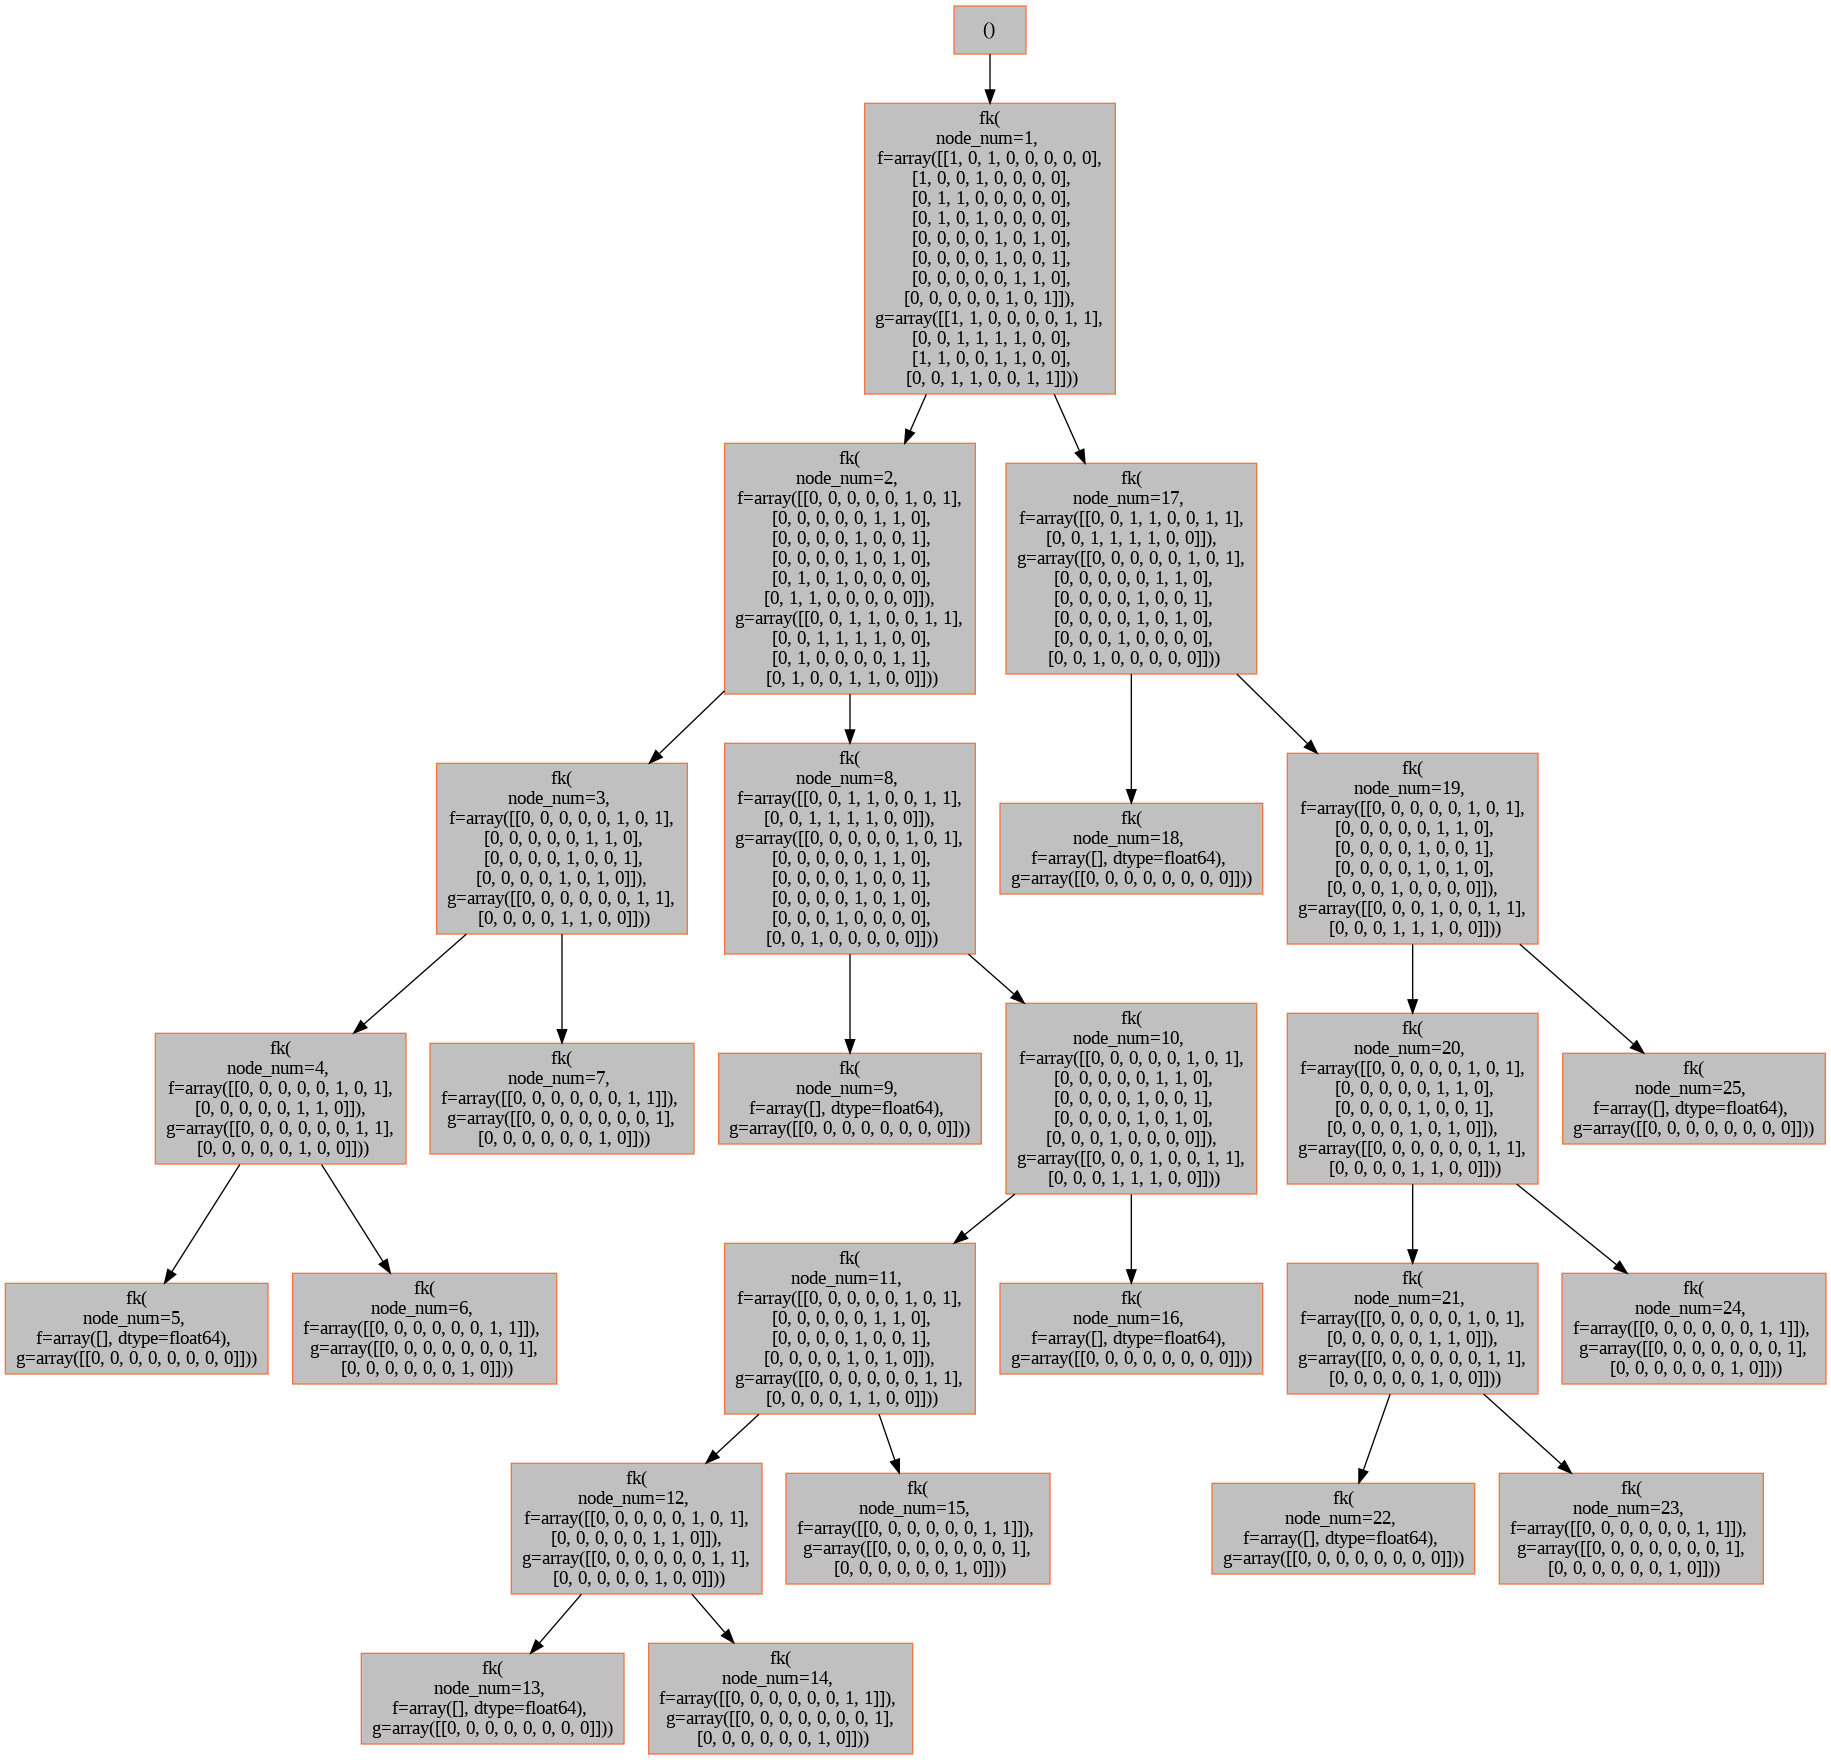
\includegraphics[width=0.62\linewidth]{figures/f2g2-fka.png}
\caption{Figures/f2, g2 in\FKA.png}
\end{subfigure}
\caption{\FKA{} recursion tree and automorphism tree of $f_2,g_2$}\label{fig:f2g2}
\end{figure}

We note that the twin classes are creating a direct product that's acting as a normal subgroup and the base group of the wreath product, supporting \ref{prop:cameron}. At Node 1, for $f_2$, the most frequent vertex is $v_1$, whose false twin partner is $v_2$. When $v_1$ is deleted and the \emph{contraction} subhypergraph $f_0\vee f_1$ is formed at Node 19 (denoted as $g$), we observe that two vertices are lost from the hypergraph. However, this is not explicitly shown in \FKA, as isolated vertices are not permitted, whereas singleton edges (edges containing a single vertex) are included.

In the corresponding \emph{deletion} subhypergraph at Node 2, we observe that no additional vertices disappear. At Node 19, the remaining two singleton edges are part of both hyperedges in their transversal. Selecting either of these singleton vertices as the next pivot vertex prunes the \textbf{L} subproblem at Node 18.

Furthermore, at Node 2, $v_2$ is selected as the most frequent vertex. The resulting contraction subhypergraph at Node 8 is identical to that at Node 17. This repetition of subproblems contributes to the enlargement of the recursion tree in \FKA.

The hypergraphs who are both read-once and $\alpha$-acyclic, have an interesting property in their primal graphs. Since cographs are distance-hereditary and they are also chordal (\ref{def:chordal}), these primal graphs are precisely the class of Ptolemaic graphs. We haven't found a classification for the families of hypergraphs when their primal graphs are chordal bipartite, or Ptolemaic in existing literature or their impact on the performance of the \FKA{} algorithm.

As we have previously discussed, Cameron proposed \cite{Cam22} that the automorphism group of cographs can be generated by taking direct products and wreath products with a symmetric group. Now, we get to see if that holds up for the corresponding clique hypergraphs.

Let's consider $G$, the disjoint union of 2 disjoint $C_4$, denoted $G_1,G_2$. The automorphism group $\Aut(G)$ must preserve the twin structure of each $C_4$ while allowing permutations between the two disjoint cycles.

We describe the structure of $\Aut(G)$ as follows:
\begin{itemize}
\item The base group $C_2\times C_2\times C_2\times C_2$ corresponds to independent actions on the twin classes $\{v_1,v_3\}$, $\{v_2,v_4\}$, $\{v_5,v_7\}$, and $\{v_6,v_8\}$.
\item The first top group $C_2$ permutes the twin classes within each connected structure independently.
\item The second top group $C_2$ permutes the two disjoint components $G_1$ and $G_2$.
\end{itemize}

Combining these, $\Aut(G)$ is isomorphic to the iterated wreath product:
\[
\Aut(G)\cong(((C_2\times C_2\times C_2\times C_2):C_2):C_2):C_2.
\]
This reflects the hierarchical structure of symmetries in $G$. This is also isomorphic to $D_4\wr S_2$, where the outer $S_2$ permutes the disjoint cycles.

Therefore, we see that our results support Cameron's proposition (\ref{prop:cameron})on the primal graph of read-once hypergraphs.

\subsubsection*{Fano Plane Hypergraph}

\begin{figure}[p]
\centering
\begin{subfigure}{\linewidth}\centering
\resizebox{\linewidth}{!}{\begin{forest}
autotree
[{\anode{1}{$v_{1}$}{$PSL(3,2)$}{Not Conformal}{Cograph, Chordal}}
  [{\anode{2}{$v_{2}$}{$S_4\text{ (Non-terminal)}$}{Not Conformal}{Cograph, Split, Chordal}}
    [{\anode{3}{$v_{3}$}{$D_8$}{$\alpha$-acyclic, ROH}{}}
      [{\anode{4}{}{$S_3$}{}{}}]
      [{\anode{5}{$v_{4}$}{$C_2$}{$\alpha$-acyclic, ROH}{}}
        [{\anode{6}{$v_{6}$}{$C_2$}{}{}}
          [{\anode{7}{}{$\{\}$}{}{}}]
          [{\anode{8}{}{$C_2$}{}{}}]
        ]
        [{\anode{9}{}{$\{\}$}{}{}}]
      ]
    ]
    [{\anode{10}{$v_{3}$}{$C_2\times C_2$}{}{Cograph}}
      [{\anode{11}{$v_{5}$}{$C_2$}{$\alpha$-acyclic, ROH}{}}
        [{\anode{12}{}{$\{\}$}{}{}}]
        [{\anode{13}{$v_{6}$}{$C_2$}{}{}}
          [{\anode{14}{}{$\{\}$}{}{}}]
          [{\anode{15}{}{$C_2$}{}{}}]
        ]
      ]
      [{\anode{16}{$v_{6}$}{$C_2$}{$\alpha$-acyclic, ROH}{}}
        [{\anode{17}{}{$S_3$}{}{}}]
        [{\anode{18}{}{$S_1$}{}{}}]
      ]
    ]
  ]
  [{\anode{19}{$v_{2}$}{$S_4\text{ (Non-terminal)}$}{Not Conformal}{Cograph, Split, Chordal}}
    [{\anode{20}{$v_{3}$}{$D_4$}{$\alpha$-acyclic, ROH}{}}
      [{\anode{21}{}{$S_3$}{}{}}]
      [{\anode{22}{$v_{4}$}{$C_2$}{$\alpha$-acyclic, ROH}{Split}}
        [{\anode{23}{$v_{6}$}{$C_2$}{}{}}
          [{\anode{24}{}{$\{\}$}{}{}}]
          [{\anode{25}{}{$C_2$}{}{}}]
        ]
        [{\anode{26}{}{$\{\}$}{}{}}]
      ]
    ]
    [{\anode{27}{$v_{3}$}{$C_2\times C_2$}{}{Cograph}}
      [{\anode{28}{$v_{5}$}{$C_2$}{$\alpha$-acyclic, ROH}{Split}}
        [{\anode{29}{}{$\{\}$}{}{}}]
        [{\anode{30}{$v_{6}$}{$C_2$}{}{}}
          [{\anode{31}{}{$\{\}$}{}{}}]
          [{\anode{32}{}{$C_2$}{}{}}]
        ]
      ]
      [{\anode{33}{$v_{6}$}{$C_2$}{$\alpha$-acyclic, ROH}{Split}}
        [{\anode{34}{}{$S_3$}{}{}}]
        [{\anode{35}{}{$C_1$}{}{}}]
      ]
    ]
  ]
]
\end{forest}
}
\caption{Automorphism Tree of Self-Transversal Fano Plane Hypergraph in \FKA}
\end{subfigure}\\[6pt]
\begin{subfigure}{\linewidth}\centering
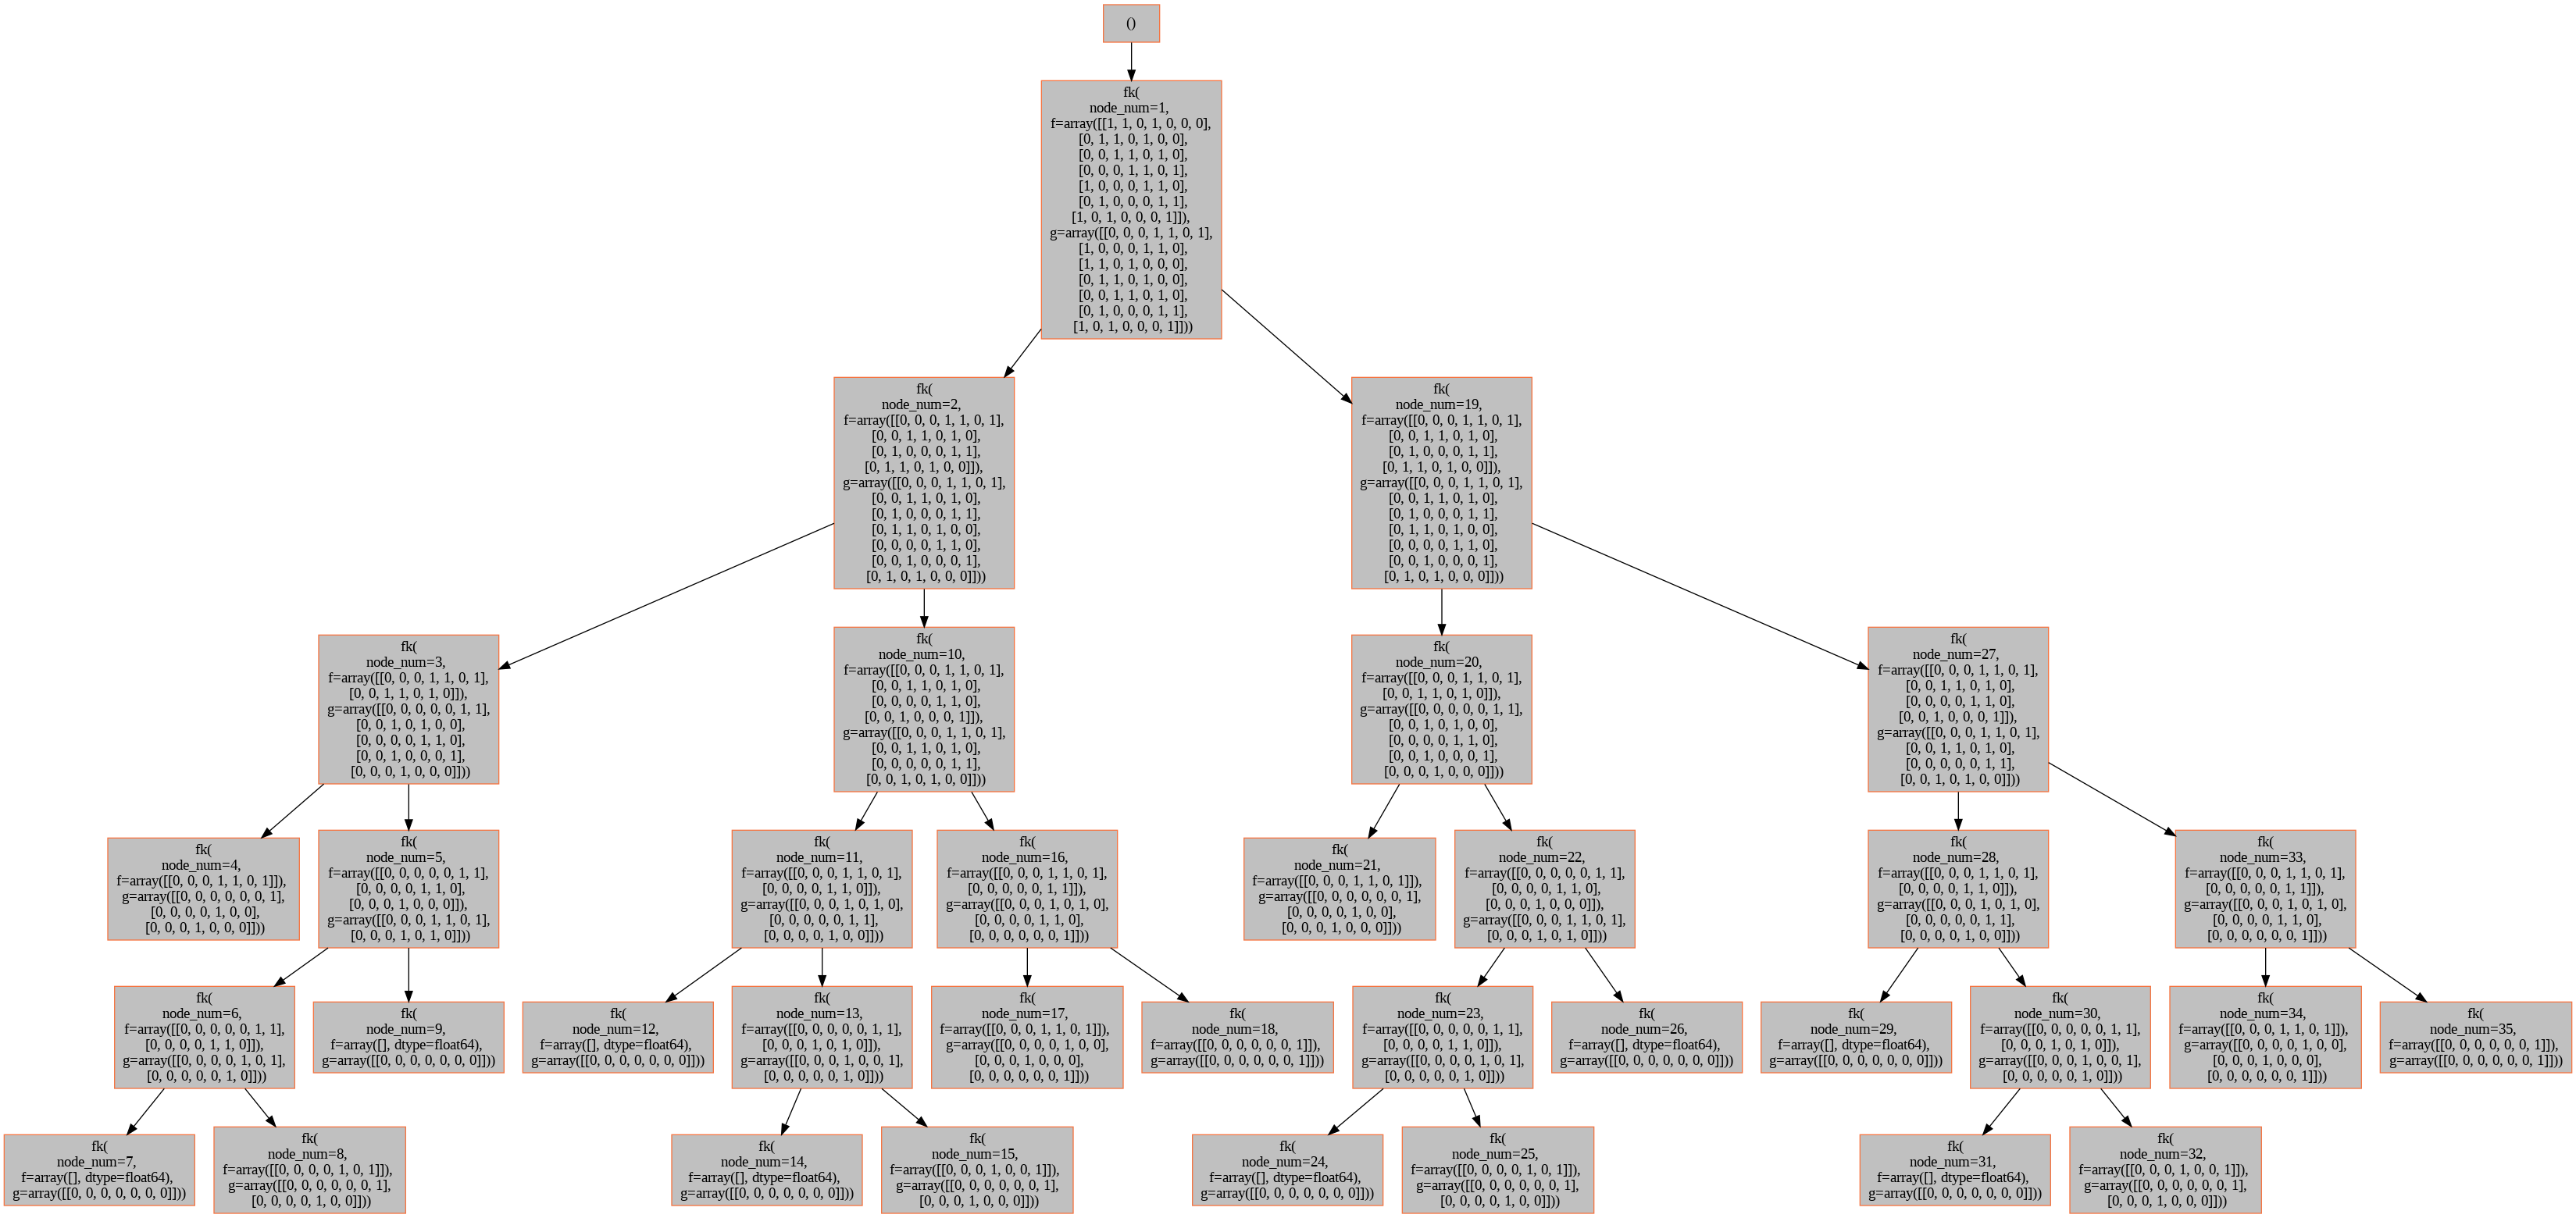
\includegraphics[width=0.8\linewidth]{figures/fano-fka.png}
\caption{Fano Plane Hypergraph in \FKA}
\end{subfigure}
\caption{\FKA{} recursion tree and automorphism tree of the Fano Plane}\label{fig:fano}
\end{figure}

Before discussing the hypergraphs from \cite{SS24}, we note the following:

\begin{observation}[\leanref{eps_three}, \leanref{eps_four}, \leanref{eps_seven}, \leanref{fano_eps}]\label{obs:fano-tight}
Let $\epsilon(n)$ be the least frequency of a most frequent vertex over transversal pairs on $n$ vertices with both hypergraphs nonempty and without the empty edge. Then $\epsilon(3)=\frac{2}{3}$, attained only by $K_3$, $\epsilon(4)=\frac{1}{2}$, and $\epsilon(7)=\frac{3}{7}$, attained by the Fano plane.
\end{observation}

The 2024 edition stated $\epsilon(7)=\frac{3}{7}$ without proof. Let $s$ be the size of a smallest edge $g$ of $G$. Counting incidences gives $s|G|\le\sum_v\deg_G v\le n\epsilon|G|$, so $s\le n\epsilon$; every minimal transversal meets $g$, so $|H|\le\sum_{v\in g}\deg_H v\le s\epsilon|H|$, so $s\epsilon\ge1$ \leanref{eps_bound}. On seven vertices $\epsilon<\frac{3}{7}$ would force $s\le2$ and then $s\epsilon<1$ \leanref{eps_seven}.

For $n=3$, we consider the hypergraph $K_3$, which is the complete 2-uniform graph on 3 vertices. It is self-transversal, with all variable frequencies equal to $\frac{2}{3}$. Since $K_3$ is the only hypergraph on 3 vertices that achieves this property, $\epsilon_3=\frac{2}{3}$, and the lower bound is tight. $K_3$ is the smallest example of a finite projective plane.

For $n=7$, we consider the Fano plane, the smallest finite projective plane with 7 lines of 3 points each on 7 vertices. The Fano plane is also self-transversal, with all variable frequencies equal to $\frac{3}{7}$.

The Fano plane is also a finite projective plane with the smallest possible number of points and lines, making it the smallest projective plane. No larger projective plane hypergraph has been shown to be self-transversal, further highlighting their distinctiveness in this context. The projective plane of order 3 is not: six of its points meet every line and contain none \leanref{pg23_not_self_dual}.

Looking at the hypergraph and its recursion tree, we see a uniform distribution of nodes in the tree. Interestingly, the primal graph of the fano plane is just the complete graph $K_7$ on 7 vertices. Any 4 vertices together form a $K_4$, which does not contain a $P_4$. However, testing primal graph properties did not reveal any additional insights due to the hypergraph being non-conformal.

While large symmetric groups have been sparse on the cases we have examined under \FKA{} recursion,the first recursion on the fano plane results in a nontrivial $S_4$ on four edges (Node 2, Node 19).

\subsubsection*{Other Cases}

The hypergraphs on 6 vertices-denoted 6-$A$, 6-$B$, 6-$C$, and 6-$D$ did not yield that much new information, but we found that apart from 6-$A$, the other 3 hypergraphs are all read-once, and $\alpha$-acyclic hypergraphs, giving us further reasons to investigate hypergraph acyclicity and it's relationship with \FKA. All four hypergraphs have the same frequency $\epsilon=\frac{1}{2}$.

The hypergraph 7-Ver. achieves a frequency $\epsilon=\frac{5}{11}$, which is suboptimal compared to the Fano plane hypergraph's $\epsilon=\frac{3}{7}$, representing a tighter frequency bound. Similarly, the hypergraph 8-Ver. achieves $\epsilon(G,H)=\frac{2}{5}$ for all vertices $i$ in both hypergraphs. This frequency, while consistent, is lower than that of the $f_2,g_2$ hypergraphs.

We note that while 8-Ver was conformal, 7-Ver was not. In fact, it was the only hypergraph from \cite{SS24} that wasn't conformal, but after some decomposition, later in the recursion tree the hypergraphs became acyclic and read-once. While on 8-Ver., we can see that the input hypergraphs maintained their conformality and also gained read-once and acyclicity properties after a second recursion.

\begin{figure}[p]
\centering
\begin{subfigure}{0.48\linewidth}\centering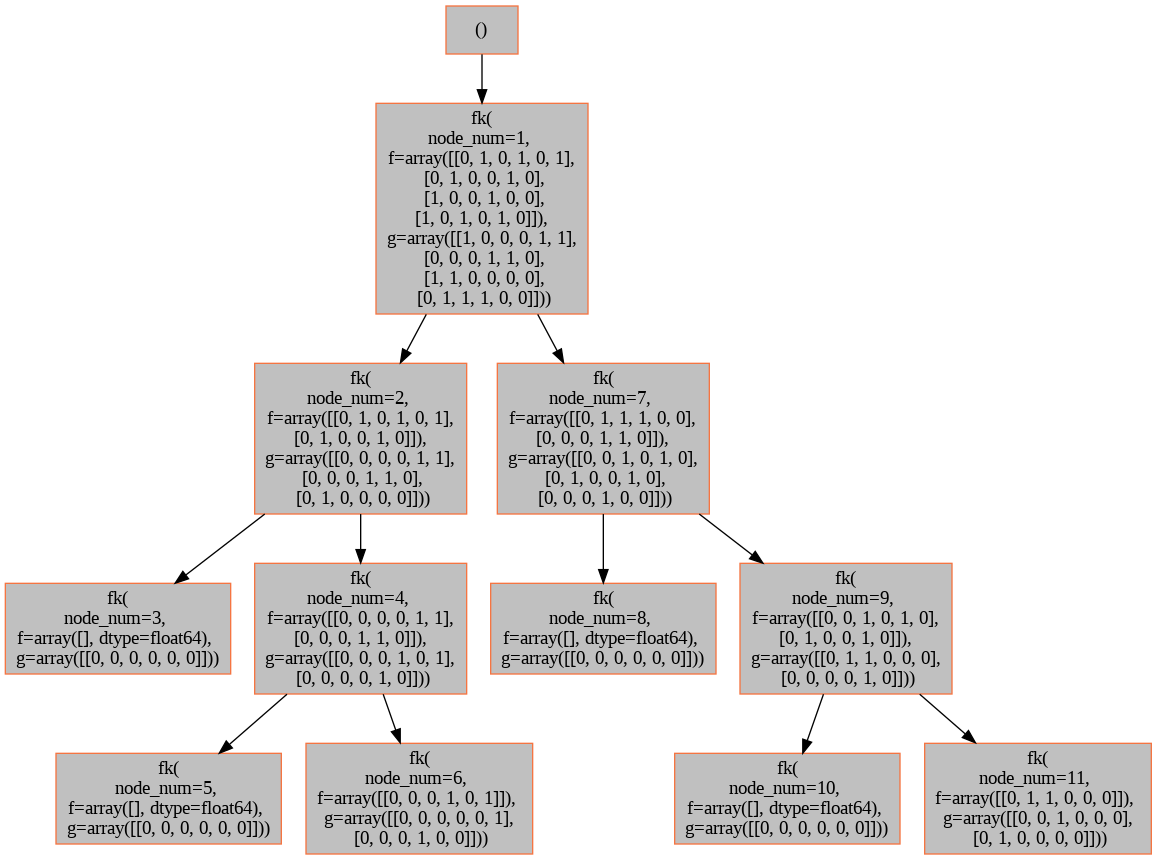
\includegraphics[width=\linewidth]{figures/6a-fka.png}\caption{Visualization of 6-$A$ in \FKA}\end{subfigure}\hfill
\begin{subfigure}{0.48\linewidth}\centering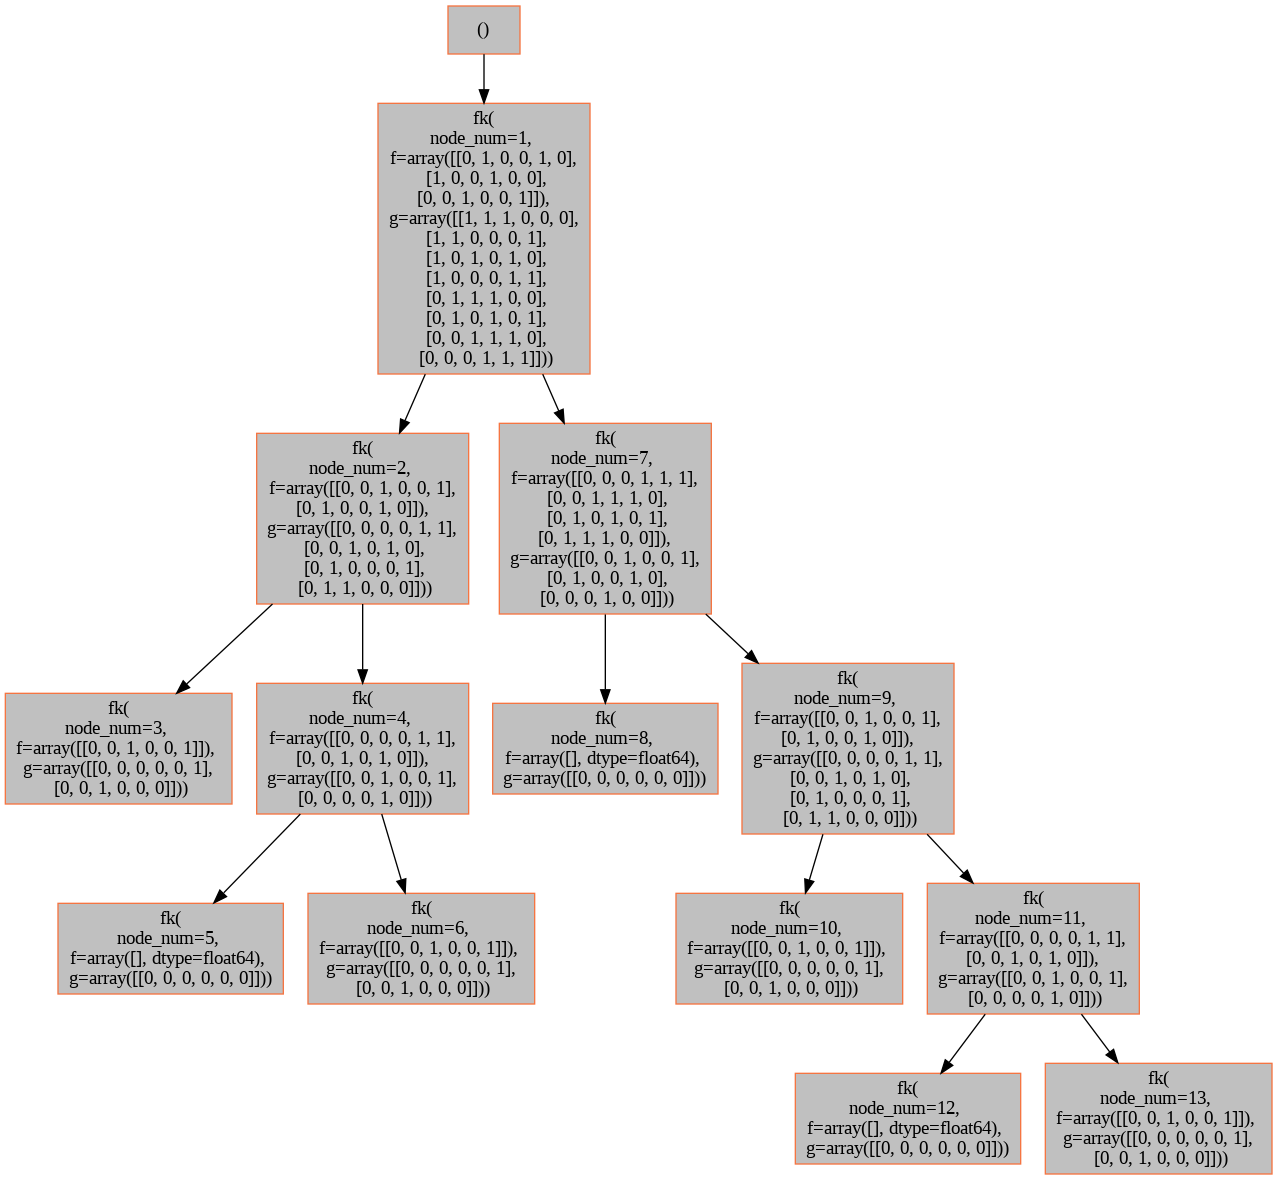
\includegraphics[width=\linewidth]{figures/6b-fka.png}\caption{Visualization of 6-$B$ in \FKA}\end{subfigure}\\[6pt]
\begin{subfigure}{0.48\linewidth}\centering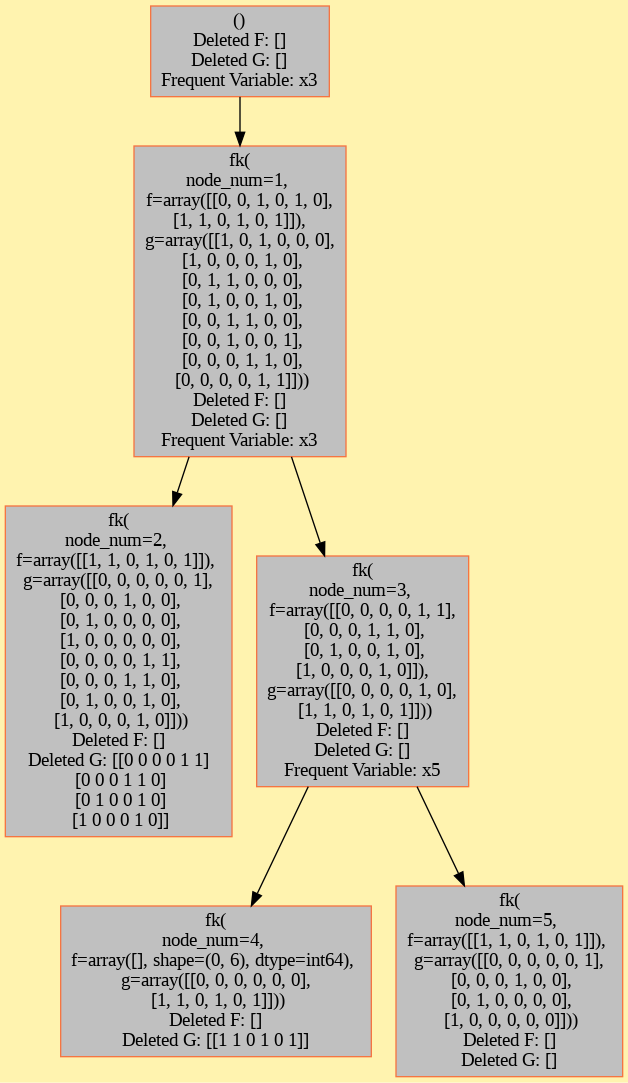
\includegraphics[width=0.85\linewidth]{figures/6c-fka.png}\caption{Visualization of 6-$C$ in \FKA}\end{subfigure}\hfill
\begin{subfigure}{0.48\linewidth}\centering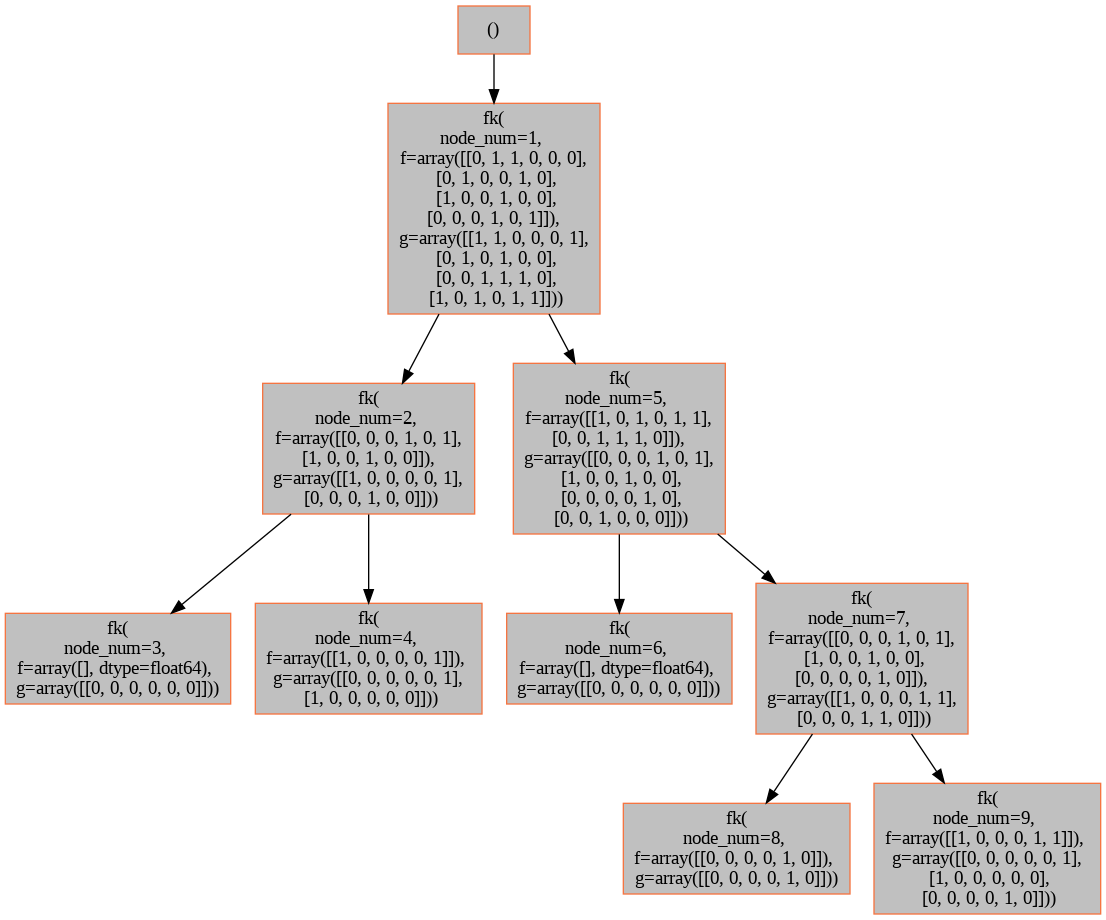
\includegraphics[width=\linewidth]{figures/6d-fka.png}\caption{Visualization of 6-$D$ in \FKA}\end{subfigure}
\caption{Visualizations of hypergraphs on 6 vertices in \FKA}
\end{figure}

\begin{figure}[p]
\centering
\begin{subfigure}{0.48\linewidth}\centering\resizebox{\linewidth}{!}{\begin{forest}
autotree
[{\anode{1}{$v_{1}$}{$C_2\times C_2$}{Conformal}{Perfect}}
  [{\anode{2}{$v_{2}$}{$C_2$}{$\alpha$-acyclic, ROH}{}}
    [{\anode{3}{}{$\{\}$}{}{}}]
    [{\anode{4}{$v_{5}$}{$C_2$}{$\alpha$-acyclic, ROH}{}}
      [{\anode{5}{}{$\{\}$}{}{}}]
      [{\anode{6}{}{$C_2$}{}{}}]
    ]
  ]
  [{\anode{7}{$v_{4}$}{$C_2$}{$\alpha$-acyclic, ROH}{}}
    [{\anode{8}{}{$\{\}$}{}{}}]
    [{\anode{9}{$v_{5}$}{$C_2$}{$\alpha$-acyclic, ROH}{}}
      [{\anode{10}{}{$\{\}$}{}{}}]
      [{\anode{11}{}{$C_2$}{}{}}]
    ]
  ]
]
\end{forest}
}\caption{Automorphism Tree of Hypergraph $6A$ from \cite{SS24} in \FKA.}\end{subfigure}\hfill
\begin{subfigure}{0.48\linewidth}\centering\resizebox{\linewidth}{!}{\begin{forest}
autotree
[{\anode{1}{$v_{1}$}{$C_2\times S_4$}{$\alpha$-acyclic, ROH}{Bipartite}}
  [{\anode{2}{$v_{2}$}{$D_4$}{}{$C_4$ graph}}
    [{\anode{3}{}{$C_2$}{}{}}]
    [{\anode{4}{$v_{5}$}{$C_2$}{}{}}
      [{\anode{5}{}{$\{\}$}{}{}}]
      [{\anode{6}{}{$C_2$}{}{}}]
    ]
  ]
  [{\anode{7}{$v_{4}$}{$D_4$}{ROH}{}}
    [{\anode{8}{}{$\{\}$}{}{}}]
    [{\anode{9}{$v_{2}$}{$D_4$}{}{$C_4$ graph}}
      [{\anode{10}{}{$C_2$}{}{}}]
      [{\anode{11}{$v_{5}$}{$C_2$}{}{}}
        [{\anode{12}{}{$\{\}$}{}{}}]
        [{\anode{13}{}{$C_2$}{}{}}]
      ]
    ]
  ]
]
\end{forest}
}\caption{Automorphism Tree of ROH Hypergraph $6B$ from \cite{SS24} in \FKA.}\end{subfigure}\\[10pt]
\begin{subfigure}{0.48\linewidth}\centering\resizebox{0.8\linewidth}{!}{\begin{forest}
autotree, for tree={font=\small}
[{\anode{1}{$v_{3}$}{$C_2\times S_4$}{ROH, $\alpha$-acyclic}{}}
  [{\anode{2}{}{$S_4$}{}{}}]
  [{\anode{3}{$v_{5}$}{$S_4$}{ROH, $\alpha$-acyclic}{Bipartite}}
    [{\anode{4}{}{$\{\}$}{}{}}]
    [{\anode{5}{}{$S_4$}{}{}}]
  ]
]
\end{forest}
}\caption{Automorphism Tree of ROH Hypergraph $6C$ from \cite{SS24} in \FKA.}\end{subfigure}\hfill
\begin{subfigure}{0.48\linewidth}\centering\resizebox{\linewidth}{!}{\begin{forest}
autotree
[{\anode{1}{$v_{2}$}{$D_4$}{ROH, $\alpha$-acyclic}{Bipartite}}
  [{\anode{2}{$v_{4}$}{$C_2$}{}{}}
    [{\anode{3}{}{$\{\}$}{}{}}]
    [{\anode{4}{}{$C_2$}{}{}}]
  ]
  [{\anode{5}{$v_{3}$}{$C_2\times C_2$}{ROH, $\alpha$-acyclic}{}}
    [{\anode{6}{}{$\{\}$}{}{}}]
    [{\anode{7}{$v_{4}$}{$C_2$}{}{}}
      [{\anode{8}{}{$C_1$}{}{}}]
      [{\anode{9}{}{$S_3$}{}{}}]
    ]
  ]
]
\end{forest}
}\caption{Automorphism Tree of Hypergraph $6D$ from \cite{SS24} in \FKA.}\end{subfigure}
\caption{\FKA{} recursion tree and automorphism tree of $6A$, $6B$, $6C$, and $6D$}
\end{figure}

\section{Future Direction}

Future research can examine the connections between hypergraph coloring, symmetry, and the \FKA{} recursion. Hypergraph $k$-coloring partitions a vertex set into $k$ sets, inducing symmetry within the coloring. However, it is unclear how \FKA{} performs when these colored hypergraphs are used as input. Investigating this relationship could provide new insights into both hypergraph coloring and the behavior of \FKA{} under symmetric constraints.

Another direction involves studying the behavior of \FKA{} on various types of acyclic hypergraphs. While $\alpha$-acyclic hypergraphs are well-studied, other forms of acyclic hypergraphs might influence the algorithm differently. Analyzing their primal graphs and how specific properties are preserved during recursion may uncover new classes of hypergraphs where \FKA{} is less efficient. Additionally, identifying hypergraphs and their transversals that cause \FKA{} to perform poorly can help expanding the upper bounds on \FKA. Recent decomposition methods have used twin vertices to simplify graphs and hypergraphs, and have proven effective in creating efficient algorithms \cite{RMN06}. Applying such techniques to \FKA{} is another avenue of research to pursue.


\backmatter%
    \addtoToC{Bibliography}
    \bibliographystyle{amsalpha}
    \bibliography{references}

%   The deposited PDF sets the appendix as an unnumbered-chapter section, which
%   is why its heading reads ".1" and its figures are numbered 5, 6, ... without
%   a chapter prefix. Reproduced as printed.

\renewcommand{\thefigure}{\arabic{figure}}
\setcounter{figure}{4}
\section{Appendix of Figures}
\clearpage

\begin{figure}[p]
\centering
\begin{subfigure}{\linewidth}\centering
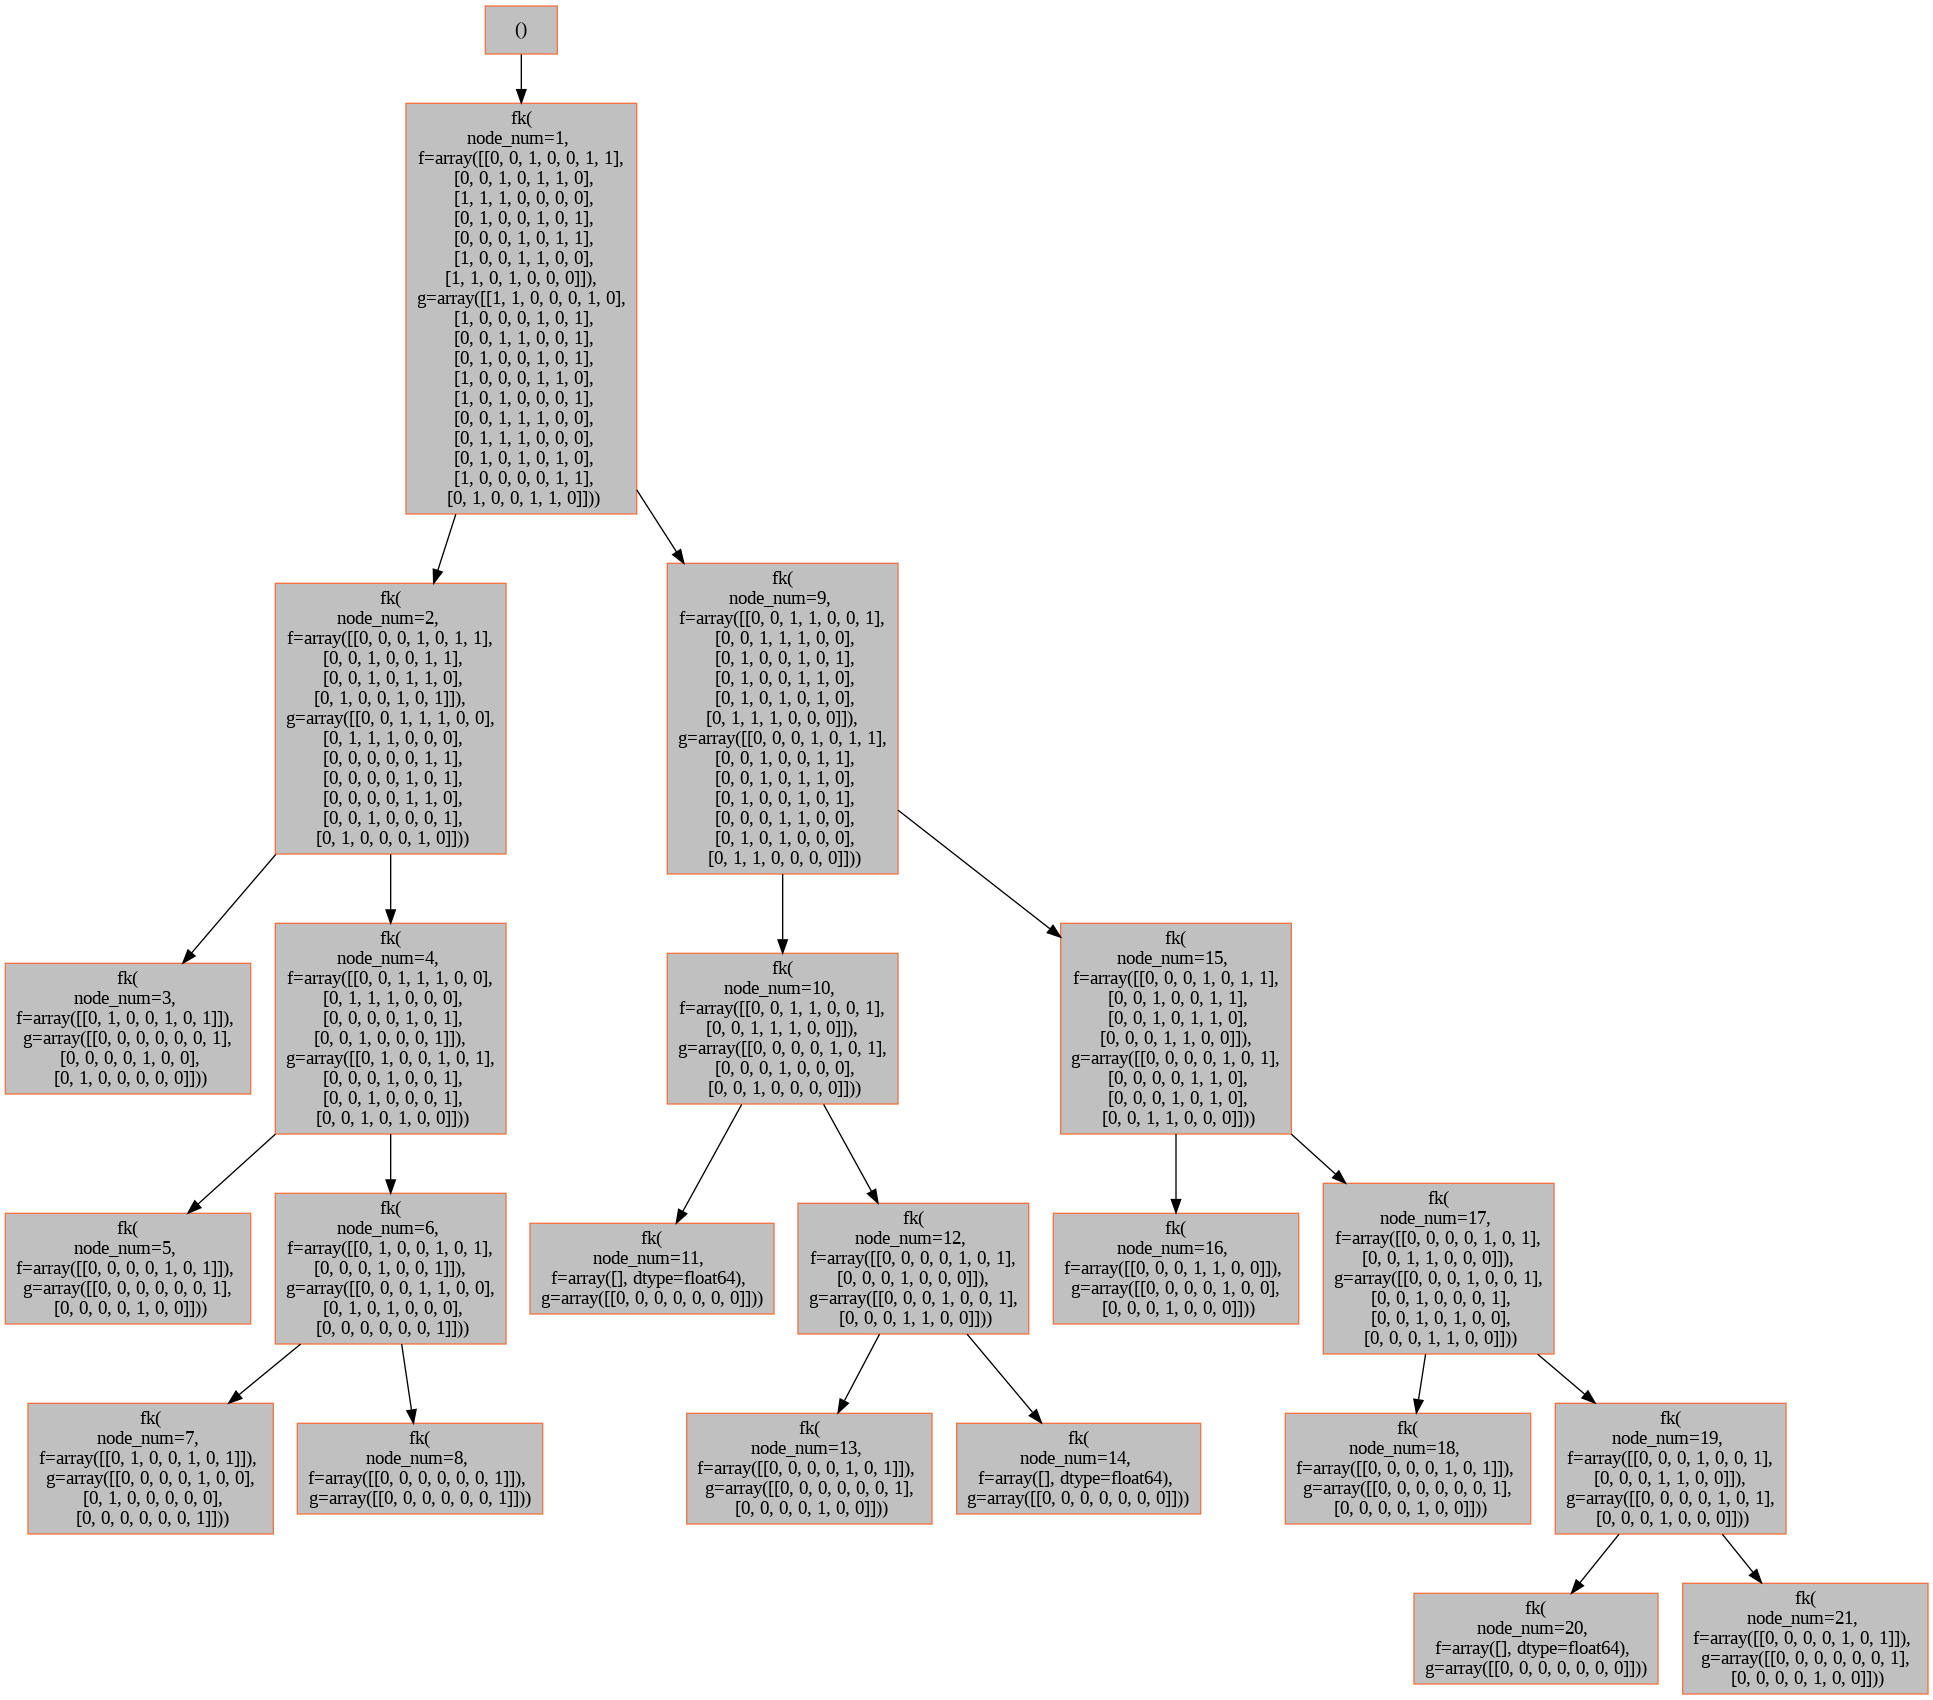
\includegraphics[width=0.62\linewidth]{figures/7ver-fka.png}
\caption{Visualization of 7-vertex Hypergraph in \FKA}
\end{subfigure}\\[4pt]
\begin{subfigure}{\linewidth}\centering
\resizebox{0.9\linewidth}{!}{\begin{forest}
autotree
[{\anode{1}{$v_{1}$}{$C_2$}{}{Cograph}}
  [{\anode{2}{$v_{6}$}{$\text{Trivial}$}{Non-Conformal}{Split, Chordal}}
    [{\anode{3}{}{$S_3$}{}{}}]
    [{\anode{4}{$v_{3}$}{$\text{Trivial}$}{Non-Conformal}{Split, Chordal, Cograph}}
      [{\anode{5}{}{$C_2$}{}{}}]
      [{\anode{6}{$v_{4}$}{$C_2$}{Read-Once, $\alpha$-acyclic}{}}
        [{\anode{7}{}{$S_3$}{}{}}]
        [{\anode{8}{}{$C_1$}{}{}}]
      ]
    ]
  ]
  [{\anode{9}{$v_{2}$}{$\text{Trivial}$}{Non-Conformal}{Split, Chordal, Cograph}}
    [{\anode{10}{$v_{3}$}{$C_2\times C_2$}{Read-Once, $\alpha$-acyclic}{Split}}
      [{\anode{11}{}{$\{\}$}{}{}}]
      [{\anode{12}{$v_{4}$}{$C_2$}{}{}}
        [{\anode{13}{}{$C_2$}{}{}}]
        [{\anode{14}{}{$\{\}$}{}{}}]
      ]
    ]
    [{\anode{15}{$v_{6}$}{}{$\alpha$-acyclic}{Bipartite}}
      [{\anode{16}{}{$C_2$}{}{}}]
      [{\anode{17}{$v_{3}$}{$D_8$}{}{$C_4$}}
        [{\anode{18}{}{$C_2$}{}{}}]
        [{\anode{19}{$v_{4}$}{$C_2$}{}{}}
          [{\anode{20}{}{$\{\}$}{}{}}]
          [{\textbf{Node: 21}\\Split vert.: $C_2$\\Hyp.:\\Graph:}]
        ]
      ]
    ]
  ]
]
\end{forest}
}
\caption{Automorphism Tree of 7-ver Hypergraph in \FKA}
\end{subfigure}
\caption{\FKA{} recursion tree and automorphism tree of 7-Ver. Hypergraph}
\end{figure}

\begin{figure}[p]
\centering
\begin{subfigure}{\linewidth}\centering
\resizebox{0.75\linewidth}{!}{\begin{forest}
autotree
[{\anode{1}{$v_{1}$}{$C_2\times D_4$}{Conformal (transversal not)}{}}
  [{\anode{2}{$v_{2}$}{$D_4$}{Conformal}{Chordal Bipartite}}
    [{\anode{3}{}{$S_3$}{}{}}]
    [{\anode{4}{$v_{6}$}{$C_2$}{Conformal}{Chordal Bipartite}}
      [{\anode{5}{$v_{5}$}{$C_2$}{}{}}
        [{\anode{6}{}{$\{\}$}{}{}}]
        [{\anode{7}{}{$C_2$}{}{}}]
      ]
      [{\anode{8}{}{$S_3$}{}{}}]
    ]
  ]
  [{\anode{9}{$v_{4}$}{$D_4$}{Conformal}{}}
    [{\anode{10}{$v_{3}$}{$C_2\times S_4$}{Read-Once, $\alpha$-acyclic}{}}
      [{\anode{11}{}{$\{\}$}{}{}}]
      [{\anode{12}{$v_{5}$}{$S_4\text{ (Non-terminal)}$}{Read-Once, $\alpha$-acyclic}{}}
        [{\anode{13}{}{$S_4$}{}{}}]
        [{\anode{14}{}{$\{\}$}{}{}}]
      ]
    ]
    [{\anode{15}{$v_{2}$}{$D_4$}{$\alpha$-acyclic}{}}
      [{\anode{16}{}{$S_3$}{}{}}]
      [{\anode{17}{$v_{6}$}{$C_2$}{$\alpha$-acyclic}{}}
        [{\anode{18}{$v_{5}$}{$C_2$}{}{}}
          [{\anode{19}{}{$\{\}$}{}{}}]
          [{\anode{20}{}{$C_2$}{}{}}]
        ]
        [{\anode{21}{}{$S_3$}{}{}}]
      ]
    ]
  ]
]
\end{forest}
}
\caption{Automorphism Tree of 8-ver in \FKA}
\end{subfigure}\\[4pt]
\begin{subfigure}{\linewidth}\centering
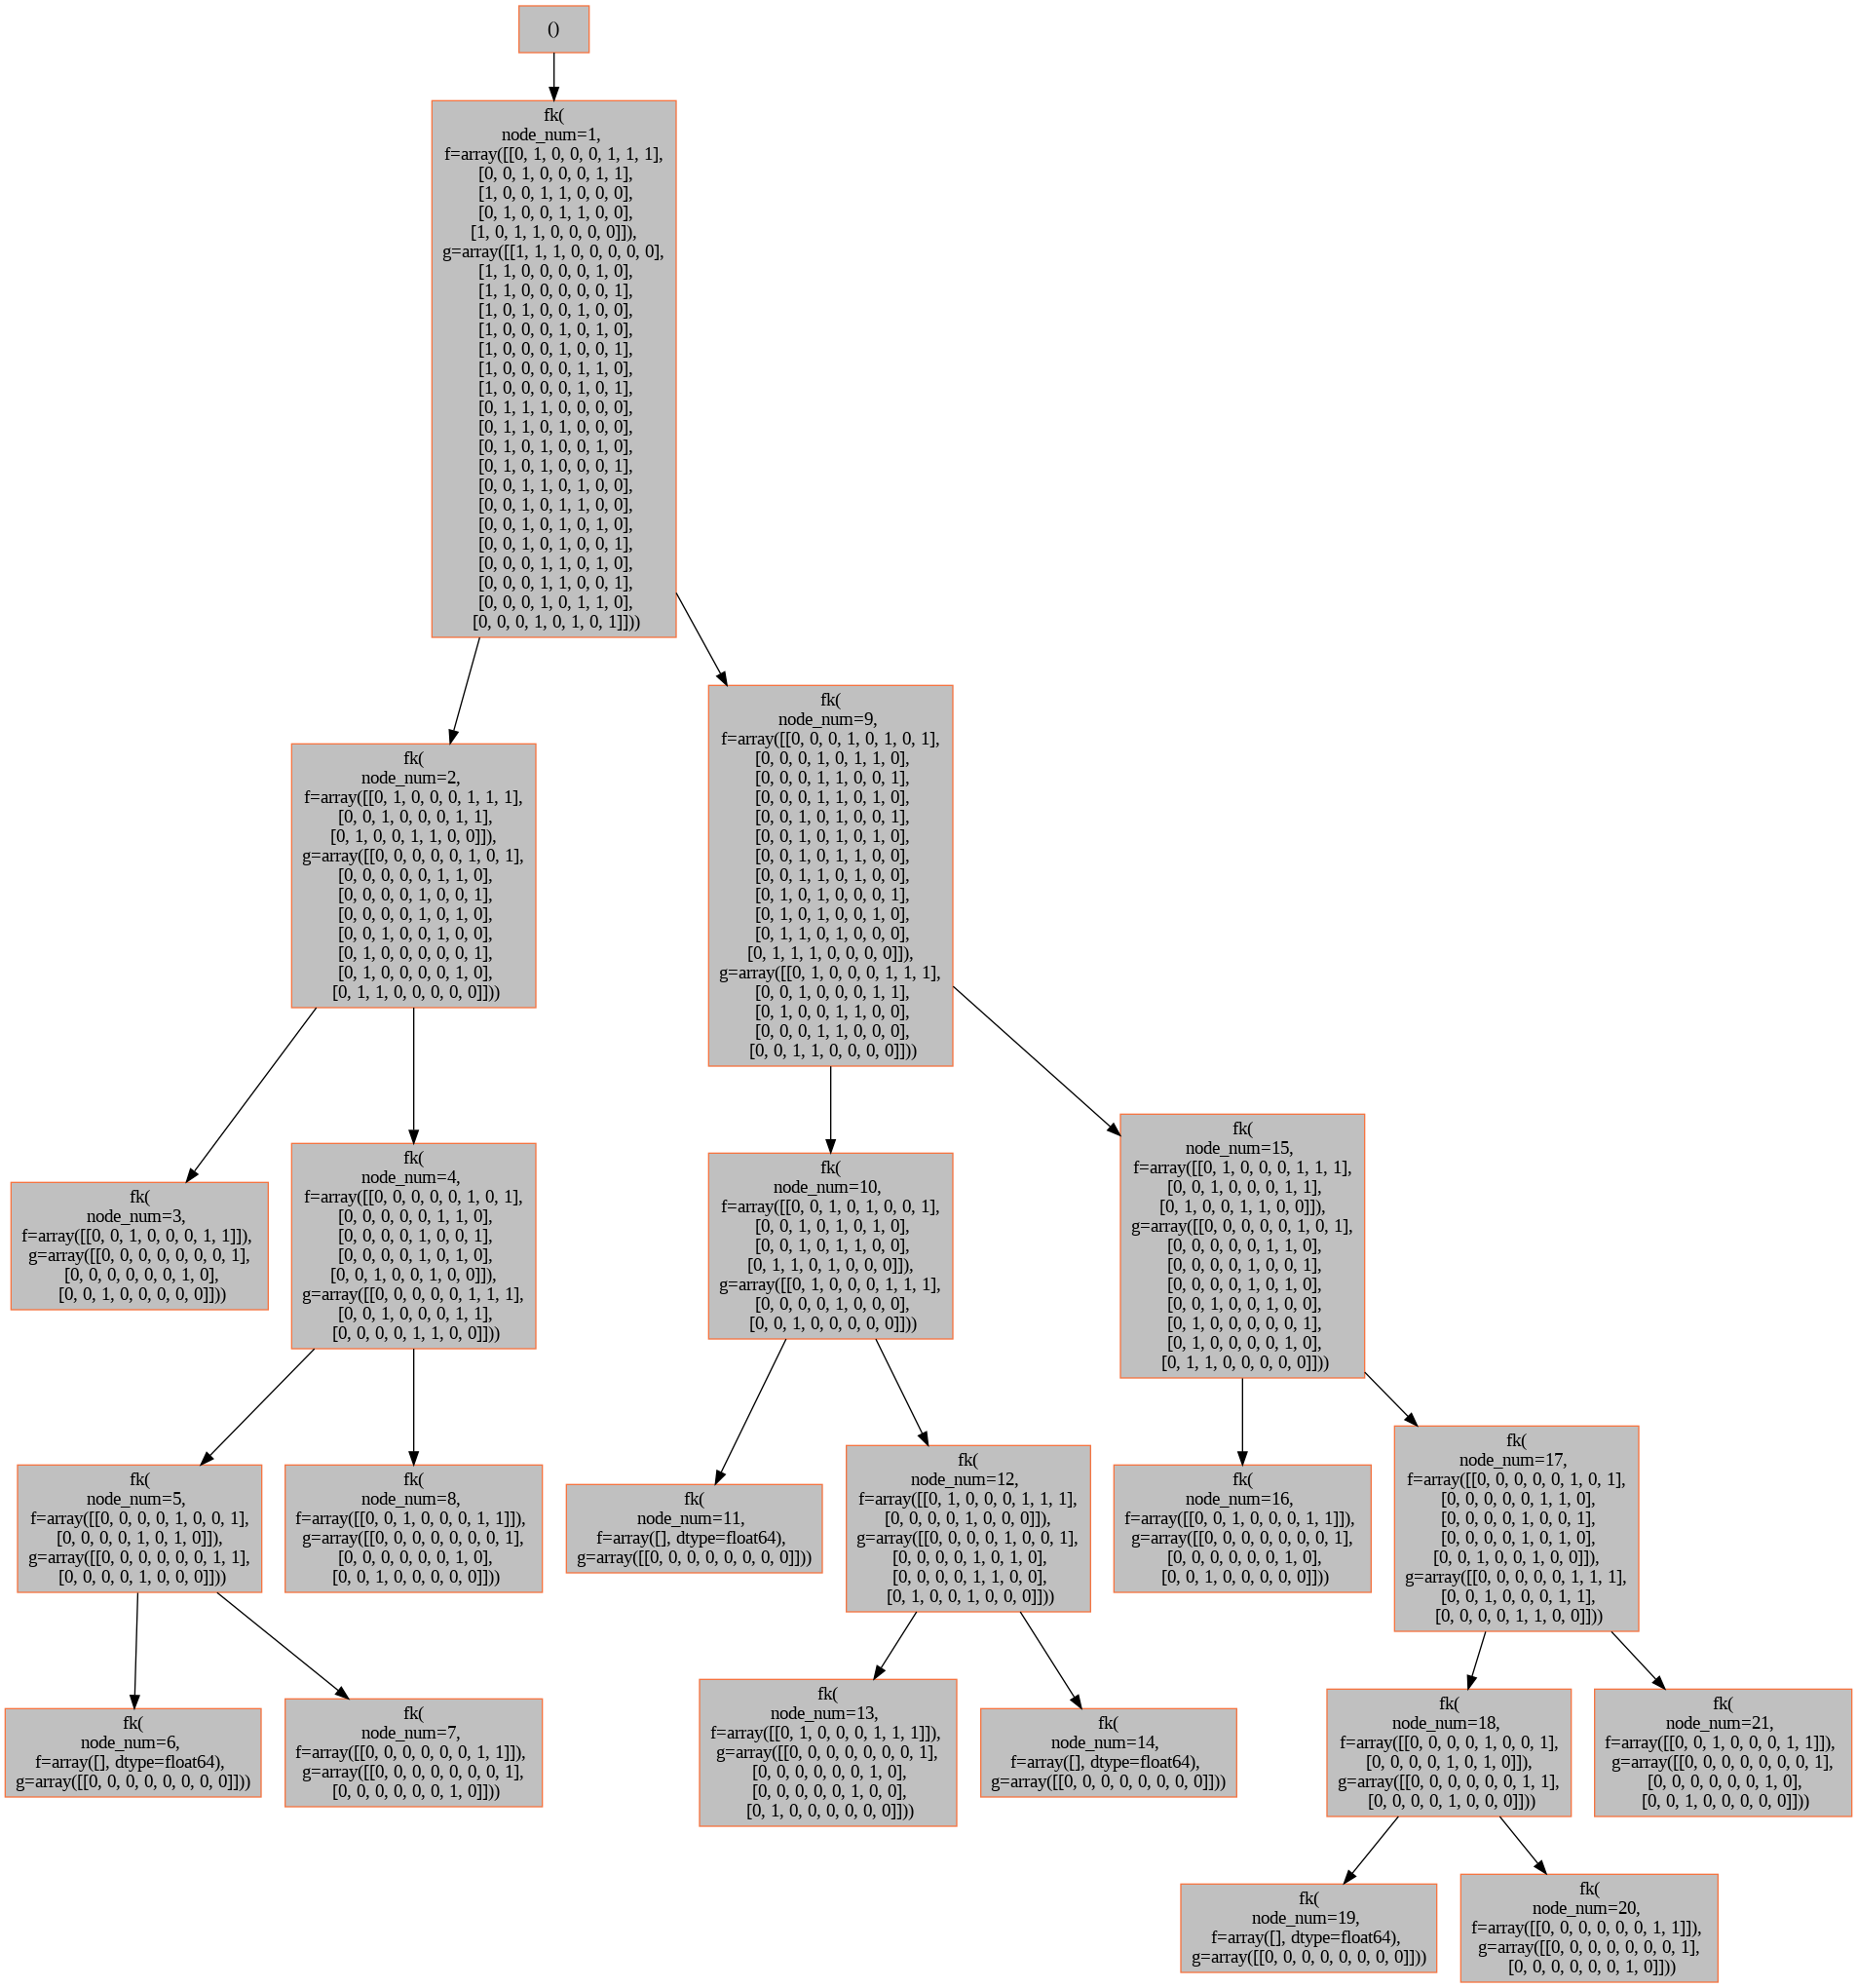
\includegraphics[width=0.62\linewidth]{figures/8ver-fka.png}
\caption{Figures/8Var in\FKA.png}
\end{subfigure}
\caption{\FKA{} recursion tree and automorphism tree of 8-ver. hypergraph}
\end{figure}

\begin{figure}[p]
\centering
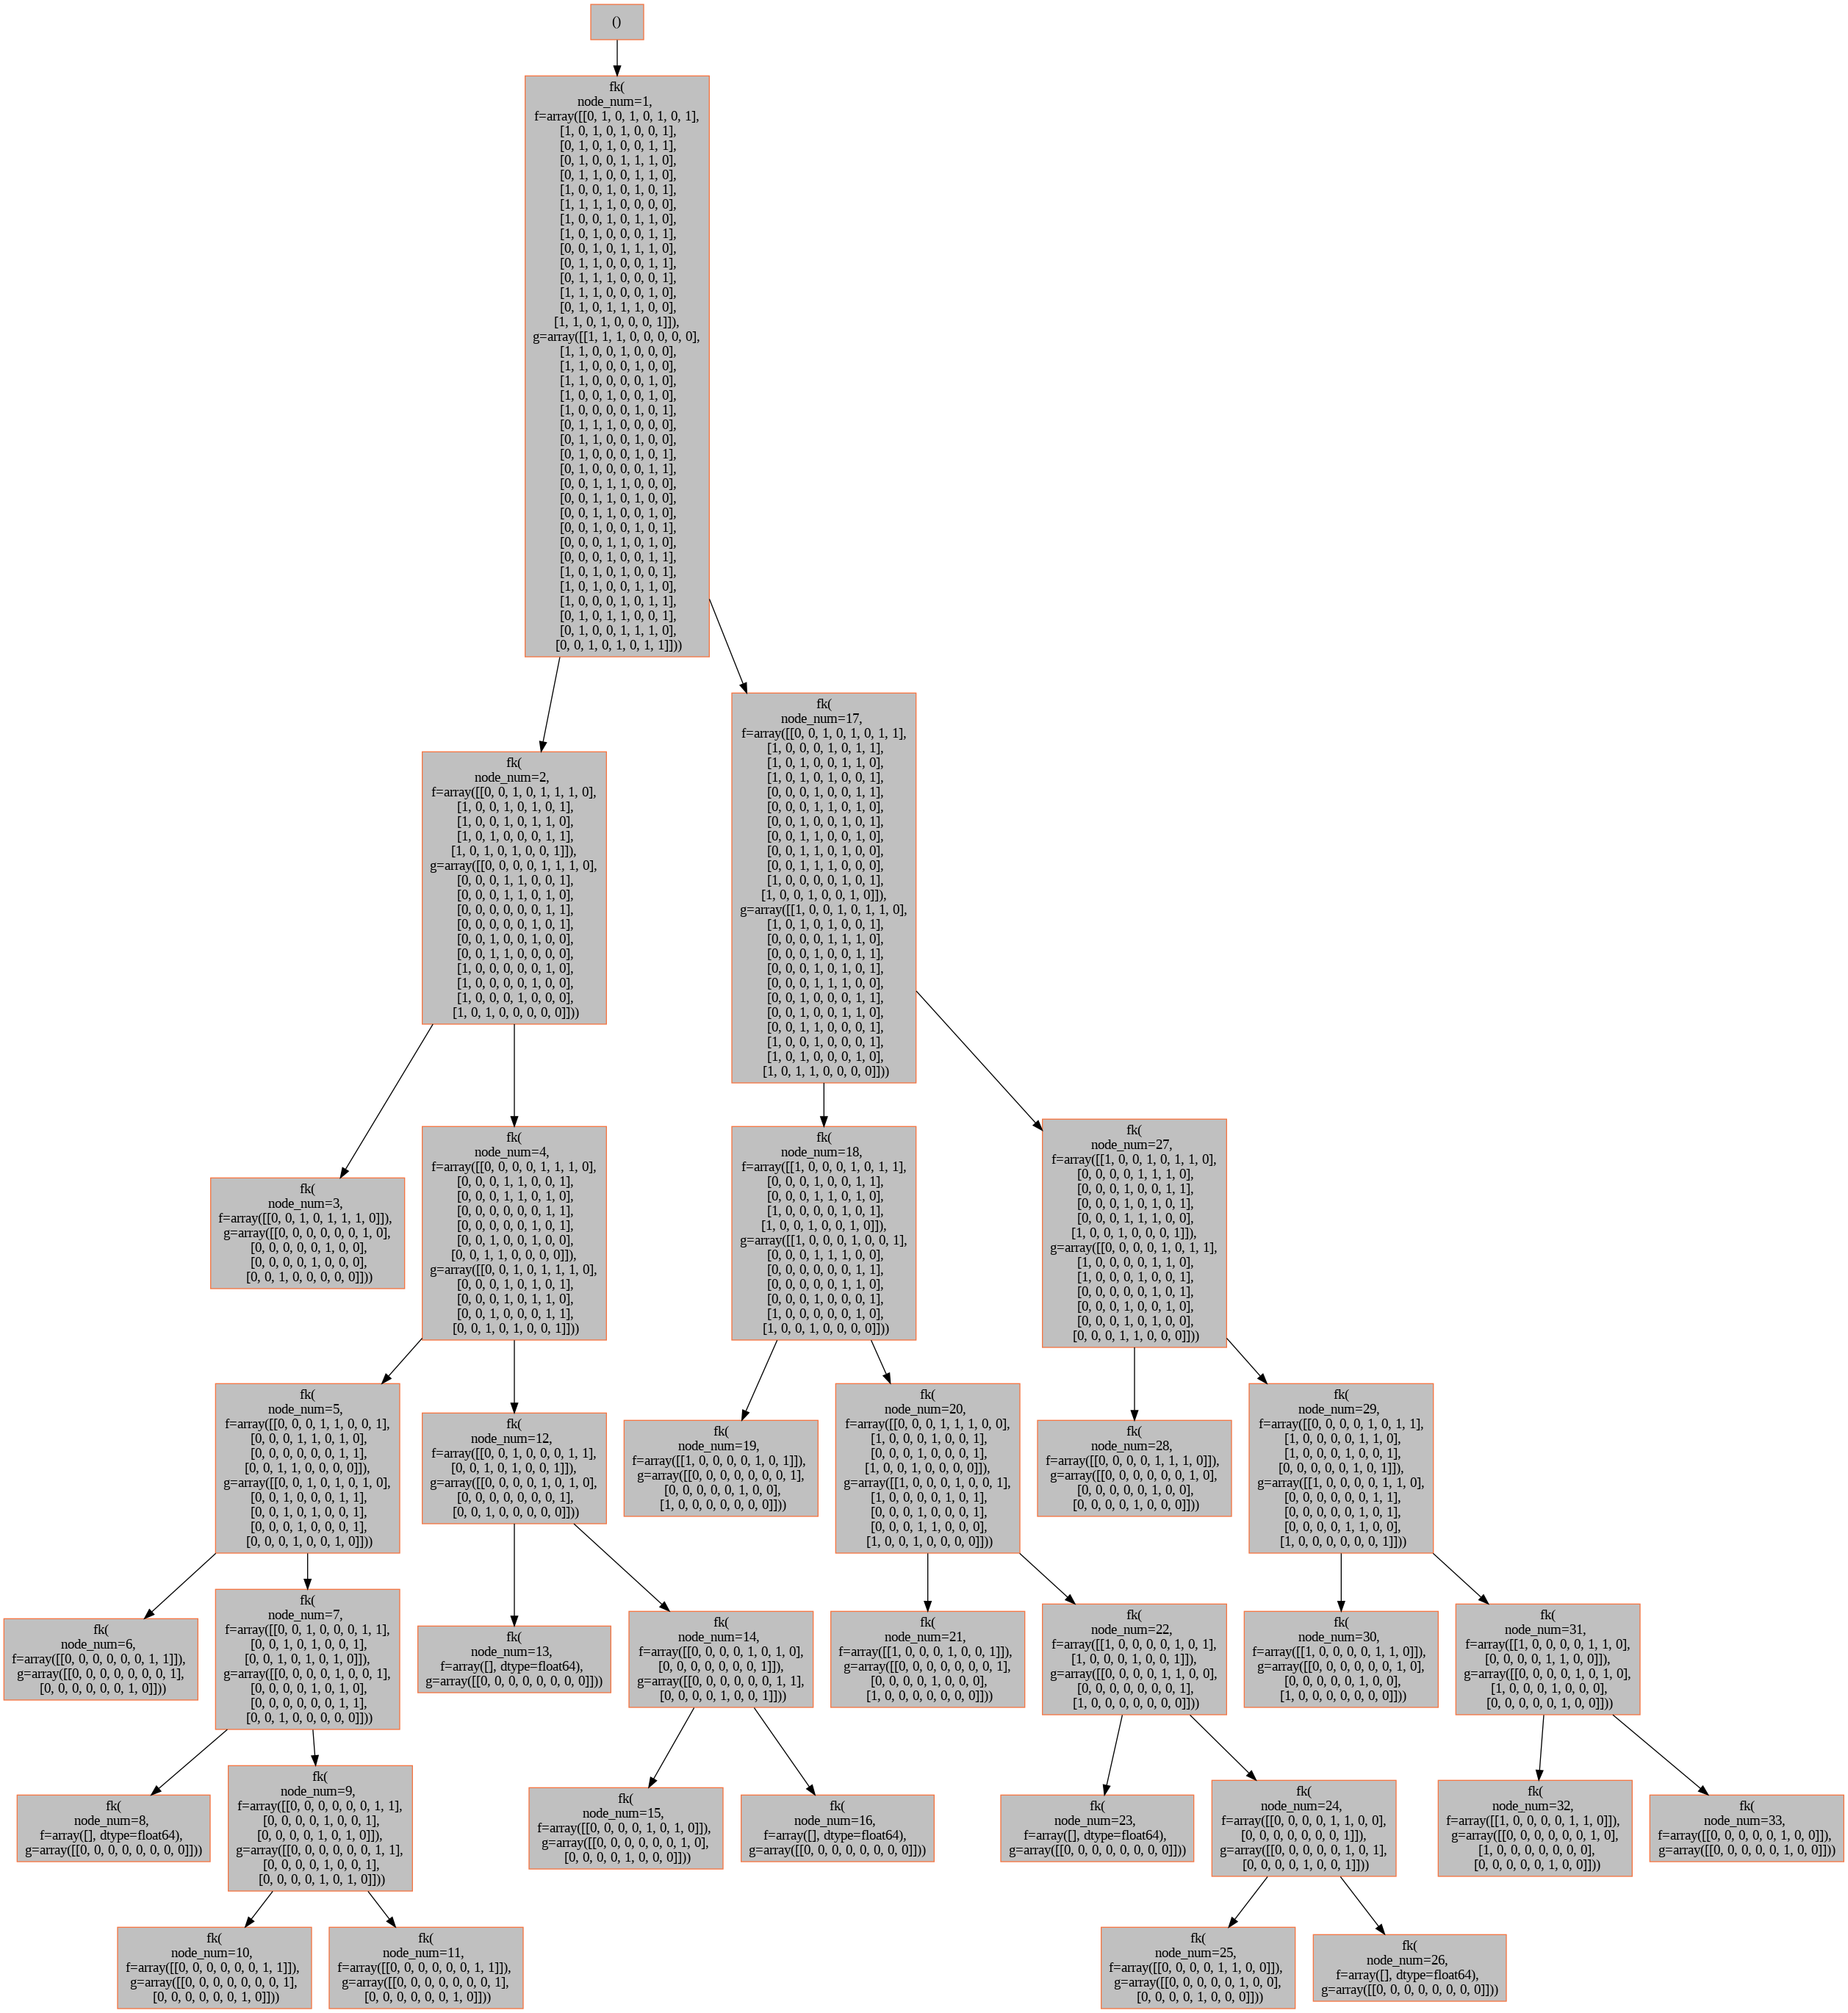
\includegraphics[width=0.75\linewidth]{figures/asym1-fka.png}
\caption{\FKA{} recursion tree on asymmetric hypergraph $Asym_1$}
\end{figure}

\begin{figure}[p]
\centering
\resizebox{\linewidth}{!}{\begin{forest}
autotree
[{\anode{1}{$v_{2}$}{$\text{Trivial}$}{}{Cograph, Chordal}}
  [{\anode{2}{$v_{8}$}{$C_2$}{}{Chordal, Cograph}}
    [{\anode{3}{}{$S_4$}{}{}}]
    [{\anode{4}{$v_{1}$}{$C_2\times C_2$}{}{Chordal, Cograph}}
      [{\anode{5}{$v_{7}$}{$C_2\times C_2$}{ROH, $\alpha$-acyclic}{}}
        [{\anode{6}{}{$C_2$}{}{}}]
        [{\anode{7}{$v_{4}$}{$C_2\times C_2$}{ROH, $\alpha$-acyclic}{}}
          [{\anode{8}{}{$\{\}$}{}{}}]
          [{\anode{9}{$v_{6}$}{$C_2$}{}{}}
            [{\anode{10}{}{$C_2$}{}{}}]
            [{\anode{11}{}{$\{\}$}{}{}}]
          ]
        ]
      ]
      [{\anode{12}{$v_{3}$}{$C_2\times C_2$}{}{Chordal, Cograph}}
        [{\anode{13}{}{$S_3$}{}{}}]
        [{\anode{14}{$v_{4}$}{$D_4$}{ROH, $\alpha$-acyclic}{}}
          [{\anode{18}{}{$C_2$}{}{}}]
          [{\anode{15}{$v_{6}$}{$C_2$}{}{}}
            [{\anode{16}{}{$\{\}$}{}{}}]
            [{\anode{17}{}{$C_2$}{}{}}]
          ]
        ]
      ]
    ]
  ]
  [{\anode{19}{$v_{1}$}{$\text{Trivial}$}{}{Cograph, Chordal}}
    [{\anode{20}{$v_{4}$}{$C_2$}{$\alpha$-acyclic}{}}
      [{\anode{21}{}{$S_3$}{}{}}]
      [{\anode{22}{$v_{8}$}{$C_2$}{}{}}
        [{\anode{23}{}{$\{\}$}{}{}}]
        [{\anode{24}{}{$C_2$}{}{}}]
      ]
    ]
    [{\anode{25}{$v_{7}$}{$\text{Trivial}$}{}{Cograph, Chordal}}
      [{\anode{26}{$v_{3}$}{$C_2\times C_2$}{}{Cograph, Chordal}}
        [{\anode{27}{}{$S_4$}{}{}}]
        [{\anode{28}{$v_{5}$}{$C_2$}{ROH, $\alpha$-acyclic}{}}
          [{\anode{29}{}{$C_1$}{}{}}]
          [{\anode{30}{}{$S_3$}{}{}}]
        ]
      ]
      [{\anode{31}{$v_{8}$}{$C_2\times C_2$}{ROH, $\alpha$-acyclic}{}}
        [{\anode{32}{$v_{5}$}{$C_2\times C_2$}{ROH, $\alpha$-acyclic}{}}
          [{\anode{33}{}{$\{\}$}{}{}}]
          [{\anode{34}{$v_{6}$}{}{}{}}
            [{\anode{35}{}{$C_2$}{}{}}]
            [{\anode{36}{}{$\{\}$}{}{}}]
          ]
        ]
        [{\anode{37}{}{$C_2$}{}{}}]
      ]
    ]
  ]
]
\end{forest}
}
\caption{Automorphism Tree of an asymmetric hypergraph \textbf{Asym}-1 in \FKA}
\end{figure}

\begin{figure}[p]
\centering
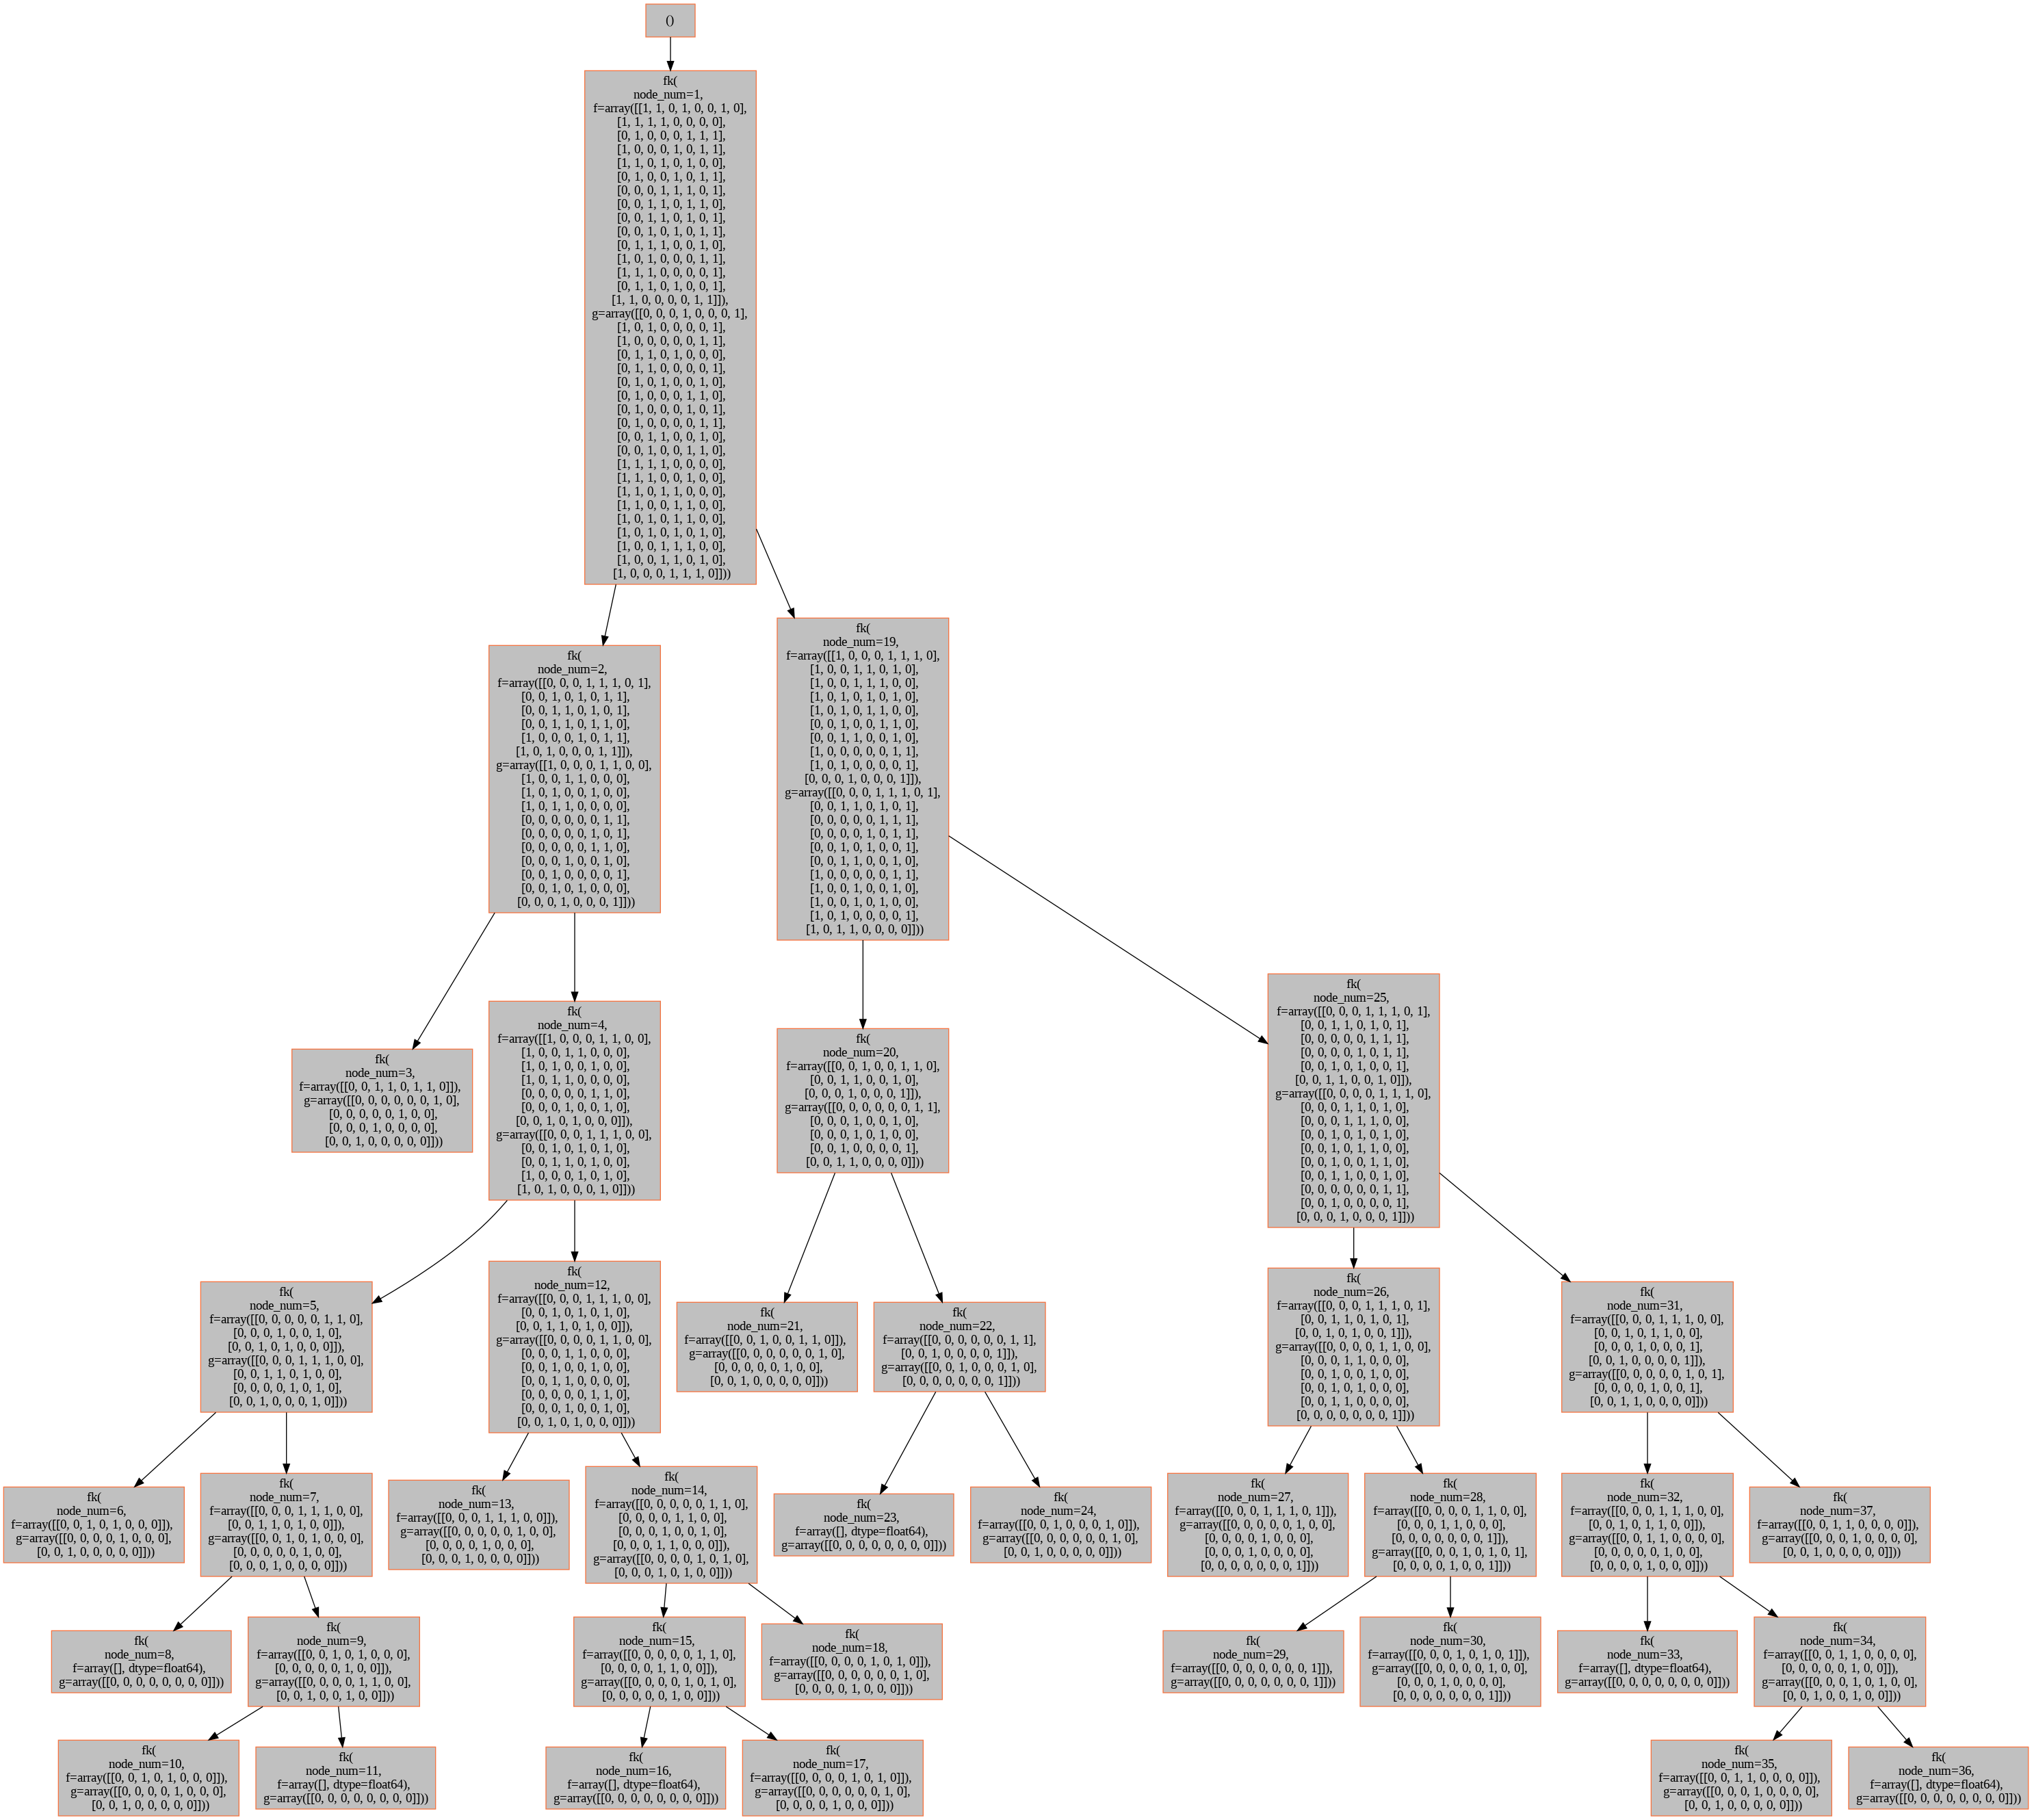
\includegraphics[width=0.9\linewidth]{figures/asym2-fka.png}
\caption{\FKA{} recursion tree on asymmetric hypergraph $Asym_2$}
\end{figure}

\begin{figure}[p]
\centering
\resizebox{\linewidth}{!}{\begin{forest}
autotree
[{\anode{1}{$v_{2}$}{$\text{Trivial}$}{}{Cograph, Split, Chordal}}
  [{\anode{2}{$v_{1}$}{$\text{Trivial}$}{}{Split, Cograph, Chordal}}
    [{\anode{3}{}{$S_4$}{}{}}]
    [{\anode{4}{$v_{6}$}{$\text{Trivial}$}{}{Split, Cograph, Chordal}}
      [{\anode{5}{$v_{4}$}{$C_2$}{}{Split, Cograph, Chordal}}
        [{\anode{6}{}{$C_2$}{}{}}]
        [{\anode{7}{$v_{3}$}{$S_3$}{}{$K_3$}}
          [{\anode{8}{}{$\{\}$}{}{}}]
          [{\anode{9}{$v_{5}$}{$C_3$}{}{$K_3$}}
            [{\anode{10}{}{$C_2$}{}{}}]
            [{\anode{11}{}{$C_2$}{}{}}]
          ]
        ]
      ]
      [{\anode{12}{$v_{3}$}{$C_2\times C_2$}{ROF, $\alpha$-acyclic}{Split}}
        [{\anode{13}{}{$\{\}$}{}{}}]
        [{\anode{14}{$v_{8}$}{$C_2$}{}{}}
          [{\anode{16}{}{$\{\}$}{}{}}]
          [{\anode{15}{}{$C_2$}{}{}}]
        ]
      ]
    ]
  ]
  [{\anode{17}{$v_{3}$}{$\text{Trivial}$}{}{Cograph, Split, Chordal}}
    [{\anode{18}{$v_{7}$}{$C_2$}{}{Cograph, Split, Chordal}}
      [{\anode{19}{}{$S_3$}{}{}}]
      [{\anode{20}{$v_{4}$}{$C_2$}{}{Cograph, Split, Chordal}}
        [{\anode{21}{}{$S_3$}{}{}}]
        [{\anode{22}{$v_{1}$}{$C_2\times C_2$}{$\alpha$-acyclic, Read-Once}{}}
          [{\anode{23}{}{$\{\}$}{}{}}]
          [{\anode{24}{$v_{8}$}{$C_2$}{}{}}
            [{\anode{25}{}{$C_2$}{}{}}]
            [{\anode{26}{}{$\{\}$}{}{}}]
          ]
        ]
      ]
    ]
    [{\anode{27}{$v_{4}$}{$\text{Trivial}$}{}{Cograph, Weakly Chordal}}
      [{\anode{28}{}{$S_3$}{}{}}]
      [{\anode{29}{$v_{8}$}{$C_2$}{}{Split, Cograph, Chordal}}
        [{\anode{30}{}{$S_3$}{}{}}]
        [{\anode{31}{$v_{5}$}{$C_2$}{ROF, $\alpha$-acyclic}{Split}}
          [{\anode{32}{}{$S_3$}{}{}}]
          [{\anode{33}{}{$C_1$}{}{}}]
        ]
      ]
    ]
  ]
]
\end{forest}
}
\caption{Automorphism Tree of an asymmetric hypergraph \textbf{Asym}-2in \FKA}
\end{figure}

%   Appendix B of the revised edition: the Lean declaration behind each statement.
%   The full register, with the printed forms of corrected statements, is thesis/CLAIMS.md.

\renewcommand{\thefigure}{\arabic{figure}}
\section*{Proof Status}
\addcontentsline{toc}{section}{Proof Status}

Every statement below is settled in Lean~4 with Mathlib, except the one marked open (\texttt{lean/HypergraphDualization} in the repository). \emph{Proved}: holds as printed, for every input. \emph{Corrected}: false or imprecise as printed in 2024; the corrected statement is proved, and the counterexample to the printed form is the last name listed. \emph{Checked}: a finite fact about named instances, proved by evaluation (\texttt{native\_decide}). \emph{Open}: not established.

{\small
\begin{longtable}{@{}>{\raggedright\arraybackslash}p{0.27\linewidth}>{\raggedright\arraybackslash}p{0.13\linewidth}>{\raggedright\arraybackslash}p{0.54\linewidth}@{}}
\textbf{Statement} & \textbf{Status} & \textbf{Lean}\\\hline
\endhead
Proposition 1.1.5 & Proved & \texttt{tr\_minimal}\\
Lemma 2.1.1 & Proved & \texttt{eq\_tr\_iff\_partition}\\
Corollary 2.1.2 & Proved & \texttt{eq\_tr\_comm}\\
Corollary 2.1.3 & Proved & \texttt{tr\_tr\_of\_sperner}, \texttt{tr\_tr}\\
Propositions 2.2.1--2.2.4 & Proved & \texttt{edges\_meet}, \texttt{support\_eq}, \texttt{card\_le\_card\_tr}, \texttt{kraft\_sum}\\
Corollary 2.3.1 & Corrected & \texttt{two\_pow\_shortest\_le}; \texttt{k3\_refutes\_printed\_cor\_2\_3\_1}\\
Lemma 2.3.2 & Proved & \texttt{exists\_frequent\_vertex}\\
Algorithm 1 decides \TransHyp & Proved & \texttt{fkA\_correct}, \texttt{conds\_of\_dual}, \texttt{dual\_split}\\
Claim 3.1.6 & Corrected & \texttt{invariant\_eq\_union\_orbits}, \texttt{orbit\_minimal}; \texttt{claim\_3\_1\_6\_counterexample}\\
Section 3.2, counts & Checked & \texttt{sperner\_four\_card}, \texttt{classes\_four}, \texttt{self\_dual\_classes\_four}, \texttt{max\_tree\_three}, \texttt{max\_tree\_four}\\
Section 3.2, $\Aut(D_{m,1})$ & Proved & \texttt{young\_aut\_singletons}\\
Section 3.2, named hypergraphs & Corrected & \texttt{*\_tr}, \texttt{table\_aut}, \texttt{table\_orbits}, \texttt{*\_freq}, \texttt{*\_splits}; \texttt{*\_printed\_*}\\
Figure 3.3(b), $\Tr(D_{3,1})$ & Corrected & \texttt{d31\_tr}\\
Lemma 3.3.1 & Corrected & \texttt{aut\_tr\_of\_sperner}, \texttt{aut\_tr\_eq\_aut\_minimal}; \texttt{lemma\_3\_3\_1\_needs\_sperner}\\
Lemma 3.3.2 & Corrected & \texttt{aut\_child\_moves\_split\_to\_isolated}, \texttt{stab\_mem\_aut\_del}, \texttt{stab\_mem\_aut\_con}\\
Lemma 3.3.3 & False & \texttt{lemma\_3\_3\_3\_false}\\
Corollary 3.3.4 & Corrected & \texttt{aut\_le\_aut\_minimal}; \texttt{cor\_3\_3\_4\_not\_iso}\\
Example of Section 3.4 & Corrected & \texttt{ex34\_corrected}\\
Observation 3.4.5 & Corrected & \texttt{primal\_children\_le}\\
Section 4.1 & Proved & \texttt{tr\_union}, \texttt{tr\_join}, \texttt{tr\_union\_disjoint}, \texttt{tr\_join\_disjoint}\\
Section 4.2, $\Tr(f_k)=g_k$, $\Tr(S_k)=r_k$ & Proved & \texttt{tr\_alt}, \texttt{tr\_coalt}\\
Section 4.2.3, recurrences & Corrected & \texttt{card\_alt\_succ}, \texttt{card\_coalt\_succ}, \texttt{alt\_counts}; \texttt{printed\_recurrence\_fails}\\
Section 4.3 & Corrected & \texttt{alt\_counts}, \texttt{alt\_shape}\\
Observation 4.4.9 & Proved & \texttt{primalAdj\_alt}, \texttt{support\_alt}\\
Section 4.4.2, distance-hereditary & Corrected & \texttt{gem\_chordal\_four}, \texttt{gem\_chordal\_five}, \texttt{gem\_not\_distance\_hereditary}\\
Lemma 4.4.13 & Proved, generalised & \texttt{twins\_mem\_aut\_cliques}, \texttt{swap\_isAut\_of\_twins}\\
Lemma 4.4.14 & Proved & \texttt{twins\_map}, \texttt{not\_trueTwin\_and\_falseTwin}\\
Section 5.2.1, instances & Corrected & \texttt{*\_dual}; \texttt{sixA\_printed\_not\_dual}, \texttt{eightVer\_printed\_not\_dual}\\
Definition 5.2.1, counts & Corrected & \texttt{kFano\_card}, \texttt{tr\_kFano\_card}; \texttt{two\_fano\_tr\_card}\\
Figures 5.1--5.6 and 5--10, tree sizes, split vertices, group orders & Checked & \texttt{*\_nodes}, \texttt{*\_tree}\\
Observation 5.2.2 & Proved & \texttt{falseTwin\_filtered}, \texttt{f2g2\_false\_twin\_filtered}\\
Observation 5.2.3 & Proved & \texttt{eps\_three}, \texttt{eps\_four}, \texttt{eps\_seven}, \texttt{fano\_eps}\\
Section 5.2.2, frequencies, self-transversality & Checked & \texttt{*\_eps}, \texttt{fano\_self\_tr}, \texttt{k3\_self\_tr}, \texttt{pg23\_not\_self\_dual}\\
\end{longtable}}

The hypergraph and graph property labels of the automorphism trees (conformal, $\alpha$-acyclic, read-once, chordal, bipartite and the like) were computed with the Python engine of the repository and are not formalized; they are reported as computations, not as proved statements.


\end{document}
